\documentclass[a4paper]{book}
\usepackage{a4wide}
\usepackage{makeidx}
\usepackage{graphicx}
\usepackage{multicol}
\usepackage{float}
\usepackage{listings}
\usepackage{color}
\usepackage{textcomp}
\usepackage{alltt}
\usepackage{times}
\usepackage{ifpdf}
\ifpdf
\usepackage[pdftex,
            pagebackref=true,
            colorlinks=true,
            linkcolor=blue,
            unicode
           ]{hyperref}
\else
\usepackage[ps2pdf,
            pagebackref=true,
            colorlinks=true,
            linkcolor=blue,
            unicode
           ]{hyperref}
\usepackage{pspicture}
\fi
\usepackage[utf8]{inputenc}
\usepackage{doxygen}
\lstset{language=C++,inputencoding=utf8,basicstyle=\footnotesize,breaklines=true,breakatwhitespace=true,tabsize=8,numbers=left }
\makeindex
\setcounter{tocdepth}{3}
\renewcommand{\footrulewidth}{0.4pt}
\begin{document}
\hypersetup{pageanchor=false}
\begin{titlepage}
\vspace*{7cm}
\begin{center}
{\Large libtmcl-\/0.2 }\\
\vspace*{1cm}
{\large Generated by Doxygen 1.6.1}\\
\vspace*{0.5cm}
{\small Mon Apr 12 14:14:09 2010}\\
\end{center}
\end{titlepage}
\clearemptydoublepage
\pagenumbering{roman}
\tableofcontents
\clearemptydoublepage
\pagenumbering{arabic}
\hypersetup{pageanchor=true}
\chapter{Trinamic Motion Control Language library}
\label{index}\hypertarget{index}{}\hypertarget{index_NOTE}{}\section{NOTE}\label{index_NOTE}
\begin{DoxyVerb}
  This documentation is created with the doxygen source code documentation generator.
  It may be regenerated by calling "make doxygen-doc" in the main source tree if
  'doxgen' (http://www.stack.nl/~dimitri/doxygen/) is installed on the system.
 \end{DoxyVerb}
\hypertarget{index_intro_sec}{}\section{Introduction}\label{index_intro_sec}
The Trinamic Motion Control Language is a set of commands for the programming of Trinamic motor controller. For the direct control of a motor-\/controller board these commands have to be translated into a command number and bundled with the command arguments, the motor address and a checksum. The command set and the details of the programming process are documented in the \char`\"{}TMCL Reference
 Manual\char`\"{} from Trinamic, which can be downloaded from \href{http://www.trinamic.com/.}{\tt http://www.trinamic.com/.}

The aim of this library is to hide the low-\/level conversion and addressing issues from the user for easier programming. A typical program using libtmcl can be as simple as the following example (error checking omitted!).


\begin{DoxyCode}
 #include <tmcl/tmcl.h>

 int main(void) {

      TMCLInterface *SerialIface; // Stores the interface of the motor-controller
       board
      TMCLMotor *Motor;     // Stores information about the motor to be controlle
      d

      // Init interface structure
      tmcl_init_interface(&SerialIface, TMCL_RSXXX, NULL, NULL, NULL, NULL);

      // Open the interface
      tmcl_open_interface(SerialIface, "/dev/ttyS0");

      // Init motor structure
      tmcl_init_motor(&Motor, SerialIface, TMCM301, 1, 0, TMCL_RSXXX);

      // Rotate motor left
      tmcl_rol(TestMotor, 100);

      // Cleanup
      tmcl_deinit_motor(&TestMotor);
      tmcl_close_interface(TestIface);
      tmcl_deinit_interface(&TestIface);

 }
\end{DoxyCode}
\hypertarget{index_install_sec}{}\section{Installation}\label{index_install_sec}
There are no special prerequisites for 'libtmcl' installation. Normally it should be enough to call:


\begin{DoxyItemize}
\item ./configure
\item make
\end{DoxyItemize}

and than with 'root' privileges:


\begin{DoxyItemize}
\item make install
\end{DoxyItemize}

For details refer to the delivered 'INSTALL' file.\hypertarget{index_step1}{}\section{\char`\"{}Let the games begin!\char`\"{}}\label{index_step1}
\hypertarget{index_firststeps}{}\subsection{First steps}\label{index_firststeps}
The first things you need to know are:


\begin{DoxyItemize}
\item The model of your trinamic controller (see \hyperlink{tmcldefs_8h_a5b6ac18c2401b554e24fe3313eda6e9a}{TMCLModel} for supported models)
\item The module address and bank of you connected motor(s) (e.g. for the first motor of module \char`\"{}1\char`\"{}: address=1, bank=0)
\item The \hyperlink{tmcldefs_8h_a3c0af0cc3f62b9e4a1daea7839da918e}{interface type}. Currently only RS232/RS485 serial interfaces are supported. Custom communication functions (open, close, read, write) may be given to \hyperlink{interface_8h_a6234d4f85bda5c0132fdecde69565ef4}{tmcl\_\-init\_\-interface()} as pointers. See example01.c in the examples directory and have a look at \hyperlink{rsXXX_8c_source}{rsXXX.c} how to do this.
\end{DoxyItemize}

With these information first initialize and open you interface struct, e.g. for a serial RS232 connection at /dev/ttyS0:


\begin{DoxyCode}
 ...
 tmcl_init_interface(&SerialIface, TMCL_RSXXX, NULL, NULL, NULL, NULL);
 tmcl_open_interface(SerialIface, "/dev/ttyS0");
 ...
\end{DoxyCode}


Remember to check the return codes for errors! 'libtmcl' functions should return values $>$=0 for success and $<$0 for failure.

After that init your motor. In this case the motor is the first motor at a TMCM-\/301 module with address \char`\"{}1\char`\"{}:


\begin{DoxyCode}
 ...
 tmcl_init_motor(&Motor, SerialIface, TMCM301, 1, 0, TMCL_RSXXX);
 ...
\end{DoxyCode}


Again: Remember to check for errors!

Some commonly used functions are defined in \hyperlink{convenience_8h}{convenience.h}, which is included from \hyperlink{tmcl_8h}{tmcl.h} by default, e.g.


\begin{DoxyItemize}
\item Activate limit/reference switches: \hyperlink{convenience_8h_abfa4f22d0004e1c6a6edae3720cbcd11}{tmcl\_\-activate\_\-limit\_\-switch(TMCLMotor$\ast$, int limit\_\-switch)};
\item Doing a refsearch: \hyperlink{convenience_8h_a002fe6b01caeb3a1c4c245e15d96d5f0}{tmcl\_\-refsearch\_\-start(TMCLMotor$\ast$)} (Remember: Reference switches have to be active for that!)
\item Move to position X: \hyperlink{convenience_8h_ade9c1b3e4ada816b7bdd76d7fd2e1639}{tmcl\_\-move\_\-to\_\-pos\_\-abs(TMCLMotor$\ast$, int position)}
\item etc.
\end{DoxyItemize}\hypertarget{index_advanced}{}\section{\char`\"{}Advanced\char`\"{} usage}\label{index_advanced}
\hypertarget{index_sendcommand}{}\subsection{Send commands}\label{index_sendcommand}
There are more commands available than what are defined in \hyperlink{convenience_8h}{convenience.h} (see TMCL Reference for details). These functions can be accessed directly by the command number defined in the TMCL reference or, for greater readability, by a command define from \hyperlink{group__TMCLComm}{tmcldefs.h}

For example: If you want to submit the \char`\"{}Move to Position (relative)\char`\"{} command \char`\"{}by hand\char`\"{} you can can use the \hyperlink{motor_8h_a0994799e6eeee41f70093c081bdc7d0a}{tmcl\_\-send\_\-command}(...) function as follows (Again: No error checking is done here, but you should do it in real code!):


\begin{DoxyCode}
  ...
  TMCLCommand command;

  command.command = TMCL_MVP;     // TMCL_MVP is defined in tmcldefs.h as command
       number "4"
  command.type    = TMCL_MVP_REL; // Relative movement. Type is not necessary for
       all commands (see TMCL reference)
  command.value   = 100;          // Move 100 steps relative to current position

  tmcl_send_command(Motor, command, NULL);   // Submit the command. We do not exp
      ect a reply, so the last argument is NULL.
  ...
\end{DoxyCode}
\hypertarget{index_axispar}{}\subsection{Axis parameter}\label{index_axispar}
Axis parameters control the way the motor is moving, e.g. speed, numer of limit switches, etc. The parameters available can be seen in \hyperlink{tmcldefs_8h}{tmcldefs.h} or the TMCL reference.

For reading and writing of axis parameters the functions \hyperlink{motor_8h_acde6e9e540c95467c08ad479ca3627cd}{tmcl\_\-get\_\-axis\_\-parameter}(...) and \hyperlink{motor_8h_a55a0a1ad09c44b1386a528b4e74f3962}{tmcl\_\-set\_\-axis\_\-parameter}(...) exists.

Examples:


\begin{DoxyCode}
  ...
  int speed;

  // Get the current speed of the motor
  speed = tmcl_get_axis_parameter(motor, TMCL_AP_CURR_SPEED);

  // Set reference search speed. This is set as a fraction of the full positionin
      g speed,
  // e.g. 2 means: half the positioning speed, 4: quarter of the full positioning
       speed, etc.
  // See TMCL reference for details
  tmcl_set_axis_parameter(motor, TMCL_AP_RFS_SPEED, 2);

  ...
\end{DoxyCode}
 
\chapter{Todo List}
\label{todo}
\hypertarget{todo}{}
\label{todo__todo000004}
\hypertarget{todo__todo000004}{}
 
\begin{DoxyDescription}
\item[Group \hyperlink{group__AxisParam}{AxisParam} ]These are not complete. 
\end{DoxyDescription}

\label{todo__todo000003}
\hypertarget{todo__todo000003}{}
 
\begin{DoxyDescription}
\item[Global \hyperlink{tmcldefs_8h_a59f577127efc6cc200f6212a19b75f62}{tmcl\_\-deinit} ]Document this. 
\end{DoxyDescription}

\label{todo__todo000002}
\hypertarget{todo__todo000002}{}
 
\begin{DoxyDescription}
\item[Global \hyperlink{tmcldefs_8h_a4843aec6363ff7b374b5fe190e17fe6e}{tmcl\_\-init} ]Document this. 
\end{DoxyDescription}

\label{todo__todo000001}
\hypertarget{todo__todo000001}{}
 
\begin{DoxyDescription}
\item[Global \hyperlink{motor_8h_a943cbb77b0d0bf244742c34211d03c17}{tmcl\_\-store\_\-axis\_\-parameter} ]: Currently broken and thus not commented 
\end{DoxyDescription}
\chapter{Module Index}
\section{Modules}
Here is a list of all modules:\begin{DoxyCompactList}
\item \contentsline{section}{Misc defines}{\pageref{group__TMCLMisc}}{}
\item \contentsline{section}{Status Codes.}{\pageref{group__StatusCodes}}{}
\item \contentsline{section}{TMCL commands.}{\pageref{group__TMCLComm}}{}
\begin{DoxyCompactList}
\item \contentsline{section}{Motion commands.}{\pageref{group__MotionComm}}{}
\item \contentsline{section}{Parameter commands.}{\pageref{group__ParComm}}{}
\item \contentsline{section}{TMCL Control Functions}{\pageref{group__CTLFuncs}}{}
\item \contentsline{section}{TMCL operation type codes.}{\pageref{group__TypeCodes}}{}
\end{DoxyCompactList}
\item \contentsline{section}{Axis Parameters}{\pageref{group__AxisParam}}{}
\begin{DoxyCompactList}
\item \contentsline{section}{Read-\/Write Parameters}{\pageref{group__RWParam}}{}
\item \contentsline{section}{Read-\/Only Parameters}{\pageref{group__ROParam}}{}
\end{DoxyCompactList}
\end{DoxyCompactList}

\chapter{Data Structure Index}
\section{Data Structures}
Here are the data structures with brief descriptions:\begin{DoxyCompactList}
\item\contentsline{section}{\hyperlink{structTMCLCommandStruct}{TMCLCommandStruct} }{\pageref{structTMCLCommandStruct}}{}
\item\contentsline{section}{\hyperlink{structTMCLDeviceStruct}{TMCLDeviceStruct} }{\pageref{structTMCLDeviceStruct}}{}
\item\contentsline{section}{\hyperlink{structTMCLInterfaceStruct}{TMCLInterfaceStruct} }{\pageref{structTMCLInterfaceStruct}}{}
\item\contentsline{section}{\hyperlink{structTMCLMotorStruct}{TMCLMotorStruct} }{\pageref{structTMCLMotorStruct}}{}
\item\contentsline{section}{\hyperlink{structTMCLReplyStruct}{TMCLReplyStruct} }{\pageref{structTMCLReplyStruct}}{}
\end{DoxyCompactList}

\chapter{File Index}
\section{File List}
Here is a list of all documented files with brief descriptions:\begin{DoxyCompactList}
\item\contentsline{section}{src/tmcl/{\bfseries config.h} }{\pageref{config_8h}}{}
\item\contentsline{section}{src/tmcl/{\bfseries convenience.c} }{\pageref{convenience_8c}}{}
\item\contentsline{section}{src/tmcl/\hyperlink{convenience_8h}{convenience.h} }{\pageref{convenience_8h}}{}
\item\contentsline{section}{src/tmcl/{\bfseries debug.h} }{\pageref{debug_8h}}{}
\item\contentsline{section}{src/tmcl/{\bfseries interface.c} }{\pageref{interface_8c}}{}
\item\contentsline{section}{src/tmcl/\hyperlink{interface_8h}{interface.h} }{\pageref{interface_8h}}{}
\item\contentsline{section}{src/tmcl/{\bfseries motor.c} }{\pageref{motor_8c}}{}
\item\contentsline{section}{src/tmcl/\hyperlink{motor_8h}{motor.h} }{\pageref{motor_8h}}{}
\item\contentsline{section}{src/tmcl/{\bfseries rsXXX.c} }{\pageref{rsXXX_8c}}{}
\item\contentsline{section}{src/tmcl/\hyperlink{rsXXX_8h}{rsXXX.h} }{\pageref{rsXXX_8h}}{}
\item\contentsline{section}{src/tmcl/\hyperlink{tmcl_8h}{tmcl.h} }{\pageref{tmcl_8h}}{}
\item\contentsline{section}{src/tmcl/\hyperlink{tmcldefs_8c}{tmcldefs.c} }{\pageref{tmcldefs_8c}}{}
\item\contentsline{section}{src/tmcl/\hyperlink{tmcldefs_8h}{tmcldefs.h} }{\pageref{tmcldefs_8h}}{}
\end{DoxyCompactList}

\chapter{Module Documentation}
\hypertarget{group__TMCLMisc}{
\section{Misc defines}
\label{group__TMCLMisc}\index{Misc defines@{Misc defines}}
}
\subsection*{Defines}
\begin{DoxyCompactItemize}
\item 
\#define \hyperlink{group__TMCLMisc_ga420f7d4b6299372763e4ac6ca6d4919a}{TMCL\_\-VERSION}~3.27
\item 
\#define \hyperlink{group__TMCLMisc_ga7d2c47709a2fef9913f9c4000d68c814}{TMCL\_\-DGRAM\_\-SIZE\_\-CAN}~7
\item 
\#define \hyperlink{group__TMCLMisc_gac361bd7186e0b9243b2a8d6dbd465660}{TMCL\_\-DGRAM\_\-SIZE\_\-IIC}~8
\item 
\#define \hyperlink{group__TMCLMisc_ga893fbfdcd1c9af739173be6476ad1696}{TMCL\_\-DGRAM\_\-SIZE\_\-RSXXX}~9
\item 
\#define \hyperlink{group__TMCLMisc_gad1cf3cae816b86b67bb50098b690a010}{TMCL\_\-MAX\_\-DGRAM\_\-SIZE}~TMCL\_\-DGRAM\_\-SIZE\_\-RSXXX
\end{DoxyCompactItemize}


\subsection{Define Documentation}
\hypertarget{group__TMCLMisc_ga7d2c47709a2fef9913f9c4000d68c814}{
\index{TMCLMisc@{TMCLMisc}!TMCL\_\-DGRAM\_\-SIZE\_\-CAN@{TMCL\_\-DGRAM\_\-SIZE\_\-CAN}}
\index{TMCL\_\-DGRAM\_\-SIZE\_\-CAN@{TMCL\_\-DGRAM\_\-SIZE\_\-CAN}!TMCLMisc@{TMCLMisc}}
\subsubsection[{TMCL\_\-DGRAM\_\-SIZE\_\-CAN}]{\setlength{\rightskip}{0pt plus 5cm}\#define TMCL\_\-DGRAM\_\-SIZE\_\-CAN~7}}
\label{group__TMCLMisc_ga7d2c47709a2fef9913f9c4000d68c814}
Datagram sizes for different busses. Datagram size for CAN bus (in bytes) 

Definition at line 39 of file tmcldefs.h.\hypertarget{group__TMCLMisc_gac361bd7186e0b9243b2a8d6dbd465660}{
\index{TMCLMisc@{TMCLMisc}!TMCL\_\-DGRAM\_\-SIZE\_\-IIC@{TMCL\_\-DGRAM\_\-SIZE\_\-IIC}}
\index{TMCL\_\-DGRAM\_\-SIZE\_\-IIC@{TMCL\_\-DGRAM\_\-SIZE\_\-IIC}!TMCLMisc@{TMCLMisc}}
\subsubsection[{TMCL\_\-DGRAM\_\-SIZE\_\-IIC}]{\setlength{\rightskip}{0pt plus 5cm}\#define TMCL\_\-DGRAM\_\-SIZE\_\-IIC~8}}
\label{group__TMCLMisc_gac361bd7186e0b9243b2a8d6dbd465660}
Datagram size for RS232/RS485 (in bytes) 

Definition at line 40 of file tmcldefs.h.\hypertarget{group__TMCLMisc_ga893fbfdcd1c9af739173be6476ad1696}{
\index{TMCLMisc@{TMCLMisc}!TMCL\_\-DGRAM\_\-SIZE\_\-RSXXX@{TMCL\_\-DGRAM\_\-SIZE\_\-RSXXX}}
\index{TMCL\_\-DGRAM\_\-SIZE\_\-RSXXX@{TMCL\_\-DGRAM\_\-SIZE\_\-RSXXX}!TMCLMisc@{TMCLMisc}}
\subsubsection[{TMCL\_\-DGRAM\_\-SIZE\_\-RSXXX}]{\setlength{\rightskip}{0pt plus 5cm}\#define TMCL\_\-DGRAM\_\-SIZE\_\-RSXXX~9}}
\label{group__TMCLMisc_ga893fbfdcd1c9af739173be6476ad1696}
Datagram size for IIC interface (in bytes) 

Definition at line 41 of file tmcldefs.h.\hypertarget{group__TMCLMisc_gad1cf3cae816b86b67bb50098b690a010}{
\index{TMCLMisc@{TMCLMisc}!TMCL\_\-MAX\_\-DGRAM\_\-SIZE@{TMCL\_\-MAX\_\-DGRAM\_\-SIZE}}
\index{TMCL\_\-MAX\_\-DGRAM\_\-SIZE@{TMCL\_\-MAX\_\-DGRAM\_\-SIZE}!TMCLMisc@{TMCLMisc}}
\subsubsection[{TMCL\_\-MAX\_\-DGRAM\_\-SIZE}]{\setlength{\rightskip}{0pt plus 5cm}\#define TMCL\_\-MAX\_\-DGRAM\_\-SIZE~TMCL\_\-DGRAM\_\-SIZE\_\-RSXXX}}
\label{group__TMCLMisc_gad1cf3cae816b86b67bb50098b690a010}
Maximum Datagram size 

Definition at line 42 of file tmcldefs.h.\hypertarget{group__TMCLMisc_ga420f7d4b6299372763e4ac6ca6d4919a}{
\index{TMCLMisc@{TMCLMisc}!TMCL\_\-VERSION@{TMCL\_\-VERSION}}
\index{TMCL\_\-VERSION@{TMCL\_\-VERSION}!TMCLMisc@{TMCLMisc}}
\subsubsection[{TMCL\_\-VERSION}]{\setlength{\rightskip}{0pt plus 5cm}\#define TMCL\_\-VERSION~3.27}}
\label{group__TMCLMisc_ga420f7d4b6299372763e4ac6ca6d4919a}
Version of TMCL standard 

Definition at line 35 of file tmcldefs.h.
\hypertarget{group__StatusCodes}{
\section{Status Codes.}
\label{group__StatusCodes}\index{Status Codes.@{Status Codes.}}
}
\subsection*{Defines}
\begin{DoxyCompactItemize}
\item 
\#define \hyperlink{group__StatusCodes_gae8f0d829c003e2daf2b4d659f10fb365}{TMCL\_\-STATUS\_\-SUCCESS}~100
\item 
\#define \hyperlink{group__StatusCodes_gae781af2133cc40ed37e50627769f75f3}{TMCL\_\-STATUS\_\-LOADED\_\-EEPROM}~101
\item 
\#define \hyperlink{group__StatusCodes_gaf588b372da14d242fc4ecb4e144b5085}{TMCL\_\-STATUS\_\-WRONG\_\-CHECKSUM}~1
\item 
\#define \hyperlink{group__StatusCodes_ga61d064f4c9f910aeb110a92489664d48}{TMCL\_\-STATUS\_\-INVALID\_\-COMMAND}~2
\item 
\#define \hyperlink{group__StatusCodes_ga9fffa59df78430367ff93cabf36f72c6}{TMCL\_\-STATUS\_\-WRONG\_\-TYPE}~3
\item 
\#define \hyperlink{group__StatusCodes_ga0d34bdc73a05adf2c2bc7e6038fb6c64}{TMCL\_\-STATUS\_\-INVALID\_\-VALUE}~4
\item 
\#define \hyperlink{group__StatusCodes_gab3c467b9ae2a256a4d62dd4e7e1922af}{TMCL\_\-STATUS\_\-EEPROM\_\-LOCKED}~5
\item 
\#define \hyperlink{group__StatusCodes_gade3c304cd225d35cad340c7fdff3a801}{TMCL\_\-STATUS\_\-COMMAND\_\-NA}~6
\end{DoxyCompactItemize}


\subsection{Detailed Description}
These are the status codes returned by the module. 

\subsection{Define Documentation}
\hypertarget{group__StatusCodes_gade3c304cd225d35cad340c7fdff3a801}{
\index{StatusCodes@{StatusCodes}!TMCL\_\-STATUS\_\-COMMAND\_\-NA@{TMCL\_\-STATUS\_\-COMMAND\_\-NA}}
\index{TMCL\_\-STATUS\_\-COMMAND\_\-NA@{TMCL\_\-STATUS\_\-COMMAND\_\-NA}!StatusCodes@{StatusCodes}}
\subsubsection[{TMCL\_\-STATUS\_\-COMMAND\_\-NA}]{\setlength{\rightskip}{0pt plus 5cm}\#define TMCL\_\-STATUS\_\-COMMAND\_\-NA~6}}
\label{group__StatusCodes_gade3c304cd225d35cad340c7fdff3a801}
Command not available 

Definition at line 61 of file tmcldefs.h.\hypertarget{group__StatusCodes_gab3c467b9ae2a256a4d62dd4e7e1922af}{
\index{StatusCodes@{StatusCodes}!TMCL\_\-STATUS\_\-EEPROM\_\-LOCKED@{TMCL\_\-STATUS\_\-EEPROM\_\-LOCKED}}
\index{TMCL\_\-STATUS\_\-EEPROM\_\-LOCKED@{TMCL\_\-STATUS\_\-EEPROM\_\-LOCKED}!StatusCodes@{StatusCodes}}
\subsubsection[{TMCL\_\-STATUS\_\-EEPROM\_\-LOCKED}]{\setlength{\rightskip}{0pt plus 5cm}\#define TMCL\_\-STATUS\_\-EEPROM\_\-LOCKED~5}}
\label{group__StatusCodes_gab3c467b9ae2a256a4d62dd4e7e1922af}
Configuration EEPROM locked 

Definition at line 60 of file tmcldefs.h.\hypertarget{group__StatusCodes_ga61d064f4c9f910aeb110a92489664d48}{
\index{StatusCodes@{StatusCodes}!TMCL\_\-STATUS\_\-INVALID\_\-COMMAND@{TMCL\_\-STATUS\_\-INVALID\_\-COMMAND}}
\index{TMCL\_\-STATUS\_\-INVALID\_\-COMMAND@{TMCL\_\-STATUS\_\-INVALID\_\-COMMAND}!StatusCodes@{StatusCodes}}
\subsubsection[{TMCL\_\-STATUS\_\-INVALID\_\-COMMAND}]{\setlength{\rightskip}{0pt plus 5cm}\#define TMCL\_\-STATUS\_\-INVALID\_\-COMMAND~2}}
\label{group__StatusCodes_ga61d064f4c9f910aeb110a92489664d48}
Invalid command 

Definition at line 57 of file tmcldefs.h.\hypertarget{group__StatusCodes_ga0d34bdc73a05adf2c2bc7e6038fb6c64}{
\index{StatusCodes@{StatusCodes}!TMCL\_\-STATUS\_\-INVALID\_\-VALUE@{TMCL\_\-STATUS\_\-INVALID\_\-VALUE}}
\index{TMCL\_\-STATUS\_\-INVALID\_\-VALUE@{TMCL\_\-STATUS\_\-INVALID\_\-VALUE}!StatusCodes@{StatusCodes}}
\subsubsection[{TMCL\_\-STATUS\_\-INVALID\_\-VALUE}]{\setlength{\rightskip}{0pt plus 5cm}\#define TMCL\_\-STATUS\_\-INVALID\_\-VALUE~4}}
\label{group__StatusCodes_ga0d34bdc73a05adf2c2bc7e6038fb6c64}
Invalid value 

Definition at line 59 of file tmcldefs.h.\hypertarget{group__StatusCodes_gae781af2133cc40ed37e50627769f75f3}{
\index{StatusCodes@{StatusCodes}!TMCL\_\-STATUS\_\-LOADED\_\-EEPROM@{TMCL\_\-STATUS\_\-LOADED\_\-EEPROM}}
\index{TMCL\_\-STATUS\_\-LOADED\_\-EEPROM@{TMCL\_\-STATUS\_\-LOADED\_\-EEPROM}!StatusCodes@{StatusCodes}}
\subsubsection[{TMCL\_\-STATUS\_\-LOADED\_\-EEPROM}]{\setlength{\rightskip}{0pt plus 5cm}\#define TMCL\_\-STATUS\_\-LOADED\_\-EEPROM~101}}
\label{group__StatusCodes_gae781af2133cc40ed37e50627769f75f3}
Command loaded into TCML program EEPROM 

Definition at line 55 of file tmcldefs.h.\hypertarget{group__StatusCodes_gae8f0d829c003e2daf2b4d659f10fb365}{
\index{StatusCodes@{StatusCodes}!TMCL\_\-STATUS\_\-SUCCESS@{TMCL\_\-STATUS\_\-SUCCESS}}
\index{TMCL\_\-STATUS\_\-SUCCESS@{TMCL\_\-STATUS\_\-SUCCESS}!StatusCodes@{StatusCodes}}
\subsubsection[{TMCL\_\-STATUS\_\-SUCCESS}]{\setlength{\rightskip}{0pt plus 5cm}\#define TMCL\_\-STATUS\_\-SUCCESS~100}}
\label{group__StatusCodes_gae8f0d829c003e2daf2b4d659f10fb365}
Successfully executed, no error 

Definition at line 54 of file tmcldefs.h.\hypertarget{group__StatusCodes_gaf588b372da14d242fc4ecb4e144b5085}{
\index{StatusCodes@{StatusCodes}!TMCL\_\-STATUS\_\-WRONG\_\-CHECKSUM@{TMCL\_\-STATUS\_\-WRONG\_\-CHECKSUM}}
\index{TMCL\_\-STATUS\_\-WRONG\_\-CHECKSUM@{TMCL\_\-STATUS\_\-WRONG\_\-CHECKSUM}!StatusCodes@{StatusCodes}}
\subsubsection[{TMCL\_\-STATUS\_\-WRONG\_\-CHECKSUM}]{\setlength{\rightskip}{0pt plus 5cm}\#define TMCL\_\-STATUS\_\-WRONG\_\-CHECKSUM~1}}
\label{group__StatusCodes_gaf588b372da14d242fc4ecb4e144b5085}
Wrong checksum 

Definition at line 56 of file tmcldefs.h.\hypertarget{group__StatusCodes_ga9fffa59df78430367ff93cabf36f72c6}{
\index{StatusCodes@{StatusCodes}!TMCL\_\-STATUS\_\-WRONG\_\-TYPE@{TMCL\_\-STATUS\_\-WRONG\_\-TYPE}}
\index{TMCL\_\-STATUS\_\-WRONG\_\-TYPE@{TMCL\_\-STATUS\_\-WRONG\_\-TYPE}!StatusCodes@{StatusCodes}}
\subsubsection[{TMCL\_\-STATUS\_\-WRONG\_\-TYPE}]{\setlength{\rightskip}{0pt plus 5cm}\#define TMCL\_\-STATUS\_\-WRONG\_\-TYPE~3}}
\label{group__StatusCodes_ga9fffa59df78430367ff93cabf36f72c6}
Wrong type 

Definition at line 58 of file tmcldefs.h.
\hypertarget{group__TMCLComm}{
\section{TMCL commands.}
\label{group__TMCLComm}\index{TMCL commands.@{TMCL commands.}}
}


Collaboration diagram for TMCL commands.:\nopagebreak
\begin{figure}[H]
\begin{center}
\leavevmode
\includegraphics[width=158pt]{group__TMCLComm}
\end{center}
\end{figure}
\subsection*{Modules}
\begin{DoxyCompactItemize}
\item 
\hyperlink{group__MotionComm}{Motion commands.}
\item 
\hyperlink{group__ParComm}{Parameter commands.}
\item 
\hyperlink{group__CTLFuncs}{TMCL Control Functions}
\item 
\hyperlink{group__TypeCodes}{TMCL operation type codes.}
\end{DoxyCompactItemize}
\subsection*{Defines}
\begin{DoxyCompactItemize}
\item 
\#define \hyperlink{group__TMCLComm_gac92473e5d6624712eb0c6e3b96e72556}{TMCL\_\-SIO}~14
\item 
\#define \hyperlink{group__TMCLComm_gaf8c91f7e3398565e620f87695e2ac8aa}{TMCL\_\-GIO}~15
\item 
\#define \hyperlink{group__TMCLComm_gaaca5ca8ff4397dde2a1d974a08dfc97d}{TMCL\_\-CALC}~19
\item 
\#define \hyperlink{group__TMCLComm_gab3445bd6ed45c31f3ed3f4db49914bbd}{TMCL\_\-COMP}~20
\item 
\#define \hyperlink{group__TMCLComm_gae98b22b798475ff3262efec2168b98a1}{TMCL\_\-JC}~21
\item 
\#define \hyperlink{group__TMCLComm_ga7516bcd7048ea0be08c282cfb65232dc}{TMCL\_\-JA}~22
\item 
\#define \hyperlink{group__TMCLComm_ga42c0ac92b2357e8833d3294b36f3ce03}{TMCL\_\-CSUB}~23
\item 
\#define \hyperlink{group__TMCLComm_gab5dbf5f5909e2c59d70ddf48dd6d68fe}{TMCL\_\-RSUB}~24
\item 
\#define \hyperlink{group__TMCLComm_ga3c134dcd5083b786adf60d3240cdee87}{TMCL\_\-WAIT}~27
\item 
\#define \hyperlink{group__TMCLComm_ga85496061c9785e9cc81068564f72d11a}{TMCL\_\-STOP}~28
\item 
\#define \hyperlink{group__TMCLComm_gaa5bb837c0debc7de9548dcd55f233cda}{TMCL\_\-SAC}~29
\item 
\#define \hyperlink{group__TMCLComm_ga98541d48d1c0ae966624414f02869164}{TMCL\_\-SCO}~30
\item 
\#define \hyperlink{group__TMCLComm_gadfdbd63f01a0e7148e6ad2ac5c7aa3f1}{TMCL\_\-GCO}~31
\item 
\#define \hyperlink{group__TMCLComm_ga55f02944bc20337ded009ae3a22a2e19}{TMCL\_\-CCO}~32
\item 
\#define \hyperlink{group__TMCLComm_gad58eac496f0281febc26c7302e0f7236}{TMCL\_\-CALCX}~33
\item 
\#define \hyperlink{group__TMCLComm_gadda3b3b029a3c196e05bc3fbb6e9f4c0}{TMCL\_\-AAP}~34
\item 
\#define \hyperlink{group__TMCLComm_gae139fce6d594db73457f09527562468c}{TMCL\_\-AGP}~35
\item 
\#define \hyperlink{group__TMCLComm_gadf8bf4f9343f77c0787ab0f131fbc92a}{TMCL\_\-CLE}~36
\item 
\#define \hyperlink{group__TMCLComm_ga452f379acd2362b3694cc2332a2ad4c0}{TMCL\_\-UF0}~64
\item 
\#define \hyperlink{group__TMCLComm_ga04c7b2800e3c01ac91161f7f680ecea0}{TMCL\_\-UF1}~65
\item 
\#define \hyperlink{group__TMCLComm_ga91dd885d4a0e3d69623d4323ca1d64df}{TMCL\_\-UF2}~66
\item 
\#define \hyperlink{group__TMCLComm_gae6e8731e90f75bc9b1218560f3640926}{TMCL\_\-UF3}~67
\item 
\#define \hyperlink{group__TMCLComm_ga24ceb335f6461de5fb3c2bd27cbb7823}{TMCL\_\-UF4}~68
\item 
\#define \hyperlink{group__TMCLComm_ga76c1ecb8e0999fac3d42b5ae4e8cc076}{TMCL\_\-UF5}~69
\item 
\#define \hyperlink{group__TMCLComm_gab5c21ab342d5fd4f5df3f5a0b286ccd1}{TMCL\_\-UF6}~70
\item 
\#define \hyperlink{group__TMCLComm_gaf16a383aac035a9bcf695ecd66ca8df2}{TMCL\_\-UF7}~71
\item 
\#define \hyperlink{group__TMCLComm_gafb1f96d5d46a081eaafdf4d8172e5417}{TMCL\_\-MVP\_\-ABS}~0
\item 
\#define \hyperlink{group__TMCLComm_gabb48ea6fc019299ba3081da7be7a1cdb}{TMCL\_\-MVP\_\-REL}~1
\item 
\#define \hyperlink{group__TMCLComm_gab1bd55bf2087a0fa580a7ed196b731b2}{TMCL\_\-MVP\_\-COORD}~2
\item 
\#define \hyperlink{group__TMCLComm_ga8ecbfcad4ab934cc6b3b4c90f07a5ba6}{TMCL\_\-RFS\_\-START}~0
\item 
\#define \hyperlink{group__TMCLComm_gadad6e89adaf4b2c93c8afd785b3aeb29}{TMCL\_\-RFS\_\-STOP}~1
\item 
\#define \hyperlink{group__TMCLComm_gadc8231e2815a936cb84f36f75da3ca02}{TMCL\_\-RFS\_\-STATUS}~2
\end{DoxyCompactItemize}


\subsection{Define Documentation}
\hypertarget{group__TMCLComm_gadda3b3b029a3c196e05bc3fbb6e9f4c0}{
\index{TMCLComm@{TMCLComm}!TMCL\_\-AAP@{TMCL\_\-AAP}}
\index{TMCL\_\-AAP@{TMCL\_\-AAP}!TMCLComm@{TMCLComm}}
\subsubsection[{TMCL\_\-AAP}]{\setlength{\rightskip}{0pt plus 5cm}\#define TMCL\_\-AAP~34}}
\label{group__TMCLComm_gadda3b3b029a3c196e05bc3fbb6e9f4c0}
Accumulator to Axis Parameter 

Definition at line 114 of file tmcldefs.h.\hypertarget{group__TMCLComm_gae139fce6d594db73457f09527562468c}{
\index{TMCLComm@{TMCLComm}!TMCL\_\-AGP@{TMCL\_\-AGP}}
\index{TMCL\_\-AGP@{TMCL\_\-AGP}!TMCLComm@{TMCLComm}}
\subsubsection[{TMCL\_\-AGP}]{\setlength{\rightskip}{0pt plus 5cm}\#define TMCL\_\-AGP~35}}
\label{group__TMCLComm_gae139fce6d594db73457f09527562468c}
Accumulator to Global Parameter 

Definition at line 115 of file tmcldefs.h.\hypertarget{group__TMCLComm_gaaca5ca8ff4397dde2a1d974a08dfc97d}{
\index{TMCLComm@{TMCLComm}!TMCL\_\-CALC@{TMCL\_\-CALC}}
\index{TMCL\_\-CALC@{TMCL\_\-CALC}!TMCLComm@{TMCLComm}}
\subsubsection[{TMCL\_\-CALC}]{\setlength{\rightskip}{0pt plus 5cm}\#define TMCL\_\-CALC~19}}
\label{group__TMCLComm_gaaca5ca8ff4397dde2a1d974a08dfc97d}
Calculate 

Definition at line 101 of file tmcldefs.h.\hypertarget{group__TMCLComm_gad58eac496f0281febc26c7302e0f7236}{
\index{TMCLComm@{TMCLComm}!TMCL\_\-CALCX@{TMCL\_\-CALCX}}
\index{TMCL\_\-CALCX@{TMCL\_\-CALCX}!TMCLComm@{TMCLComm}}
\subsubsection[{TMCL\_\-CALCX}]{\setlength{\rightskip}{0pt plus 5cm}\#define TMCL\_\-CALCX~33}}
\label{group__TMCLComm_gad58eac496f0281febc26c7302e0f7236}
Calculate using the X register 

Definition at line 113 of file tmcldefs.h.\hypertarget{group__TMCLComm_ga55f02944bc20337ded009ae3a22a2e19}{
\index{TMCLComm@{TMCLComm}!TMCL\_\-CCO@{TMCL\_\-CCO}}
\index{TMCL\_\-CCO@{TMCL\_\-CCO}!TMCLComm@{TMCLComm}}
\subsubsection[{TMCL\_\-CCO}]{\setlength{\rightskip}{0pt plus 5cm}\#define TMCL\_\-CCO~32}}
\label{group__TMCLComm_ga55f02944bc20337ded009ae3a22a2e19}
Capture Coordinate 

Definition at line 112 of file tmcldefs.h.\hypertarget{group__TMCLComm_gadf8bf4f9343f77c0787ab0f131fbc92a}{
\index{TMCLComm@{TMCLComm}!TMCL\_\-CLE@{TMCL\_\-CLE}}
\index{TMCL\_\-CLE@{TMCL\_\-CLE}!TMCLComm@{TMCLComm}}
\subsubsection[{TMCL\_\-CLE}]{\setlength{\rightskip}{0pt plus 5cm}\#define TMCL\_\-CLE~36}}
\label{group__TMCLComm_gadf8bf4f9343f77c0787ab0f131fbc92a}
Clear Error Flag 

Definition at line 116 of file tmcldefs.h.\hypertarget{group__TMCLComm_gab3445bd6ed45c31f3ed3f4db49914bbd}{
\index{TMCLComm@{TMCLComm}!TMCL\_\-COMP@{TMCL\_\-COMP}}
\index{TMCL\_\-COMP@{TMCL\_\-COMP}!TMCLComm@{TMCLComm}}
\subsubsection[{TMCL\_\-COMP}]{\setlength{\rightskip}{0pt plus 5cm}\#define TMCL\_\-COMP~20}}
\label{group__TMCLComm_gab3445bd6ed45c31f3ed3f4db49914bbd}
Compare 

Definition at line 102 of file tmcldefs.h.\hypertarget{group__TMCLComm_ga42c0ac92b2357e8833d3294b36f3ce03}{
\index{TMCLComm@{TMCLComm}!TMCL\_\-CSUB@{TMCL\_\-CSUB}}
\index{TMCL\_\-CSUB@{TMCL\_\-CSUB}!TMCLComm@{TMCLComm}}
\subsubsection[{TMCL\_\-CSUB}]{\setlength{\rightskip}{0pt plus 5cm}\#define TMCL\_\-CSUB~23}}
\label{group__TMCLComm_ga42c0ac92b2357e8833d3294b36f3ce03}
Call Subroutine 

Definition at line 105 of file tmcldefs.h.\hypertarget{group__TMCLComm_gadfdbd63f01a0e7148e6ad2ac5c7aa3f1}{
\index{TMCLComm@{TMCLComm}!TMCL\_\-GCO@{TMCL\_\-GCO}}
\index{TMCL\_\-GCO@{TMCL\_\-GCO}!TMCLComm@{TMCLComm}}
\subsubsection[{TMCL\_\-GCO}]{\setlength{\rightskip}{0pt plus 5cm}\#define TMCL\_\-GCO~31}}
\label{group__TMCLComm_gadfdbd63f01a0e7148e6ad2ac5c7aa3f1}
Get Coordinate 

Definition at line 111 of file tmcldefs.h.\hypertarget{group__TMCLComm_gaf8c91f7e3398565e620f87695e2ac8aa}{
\index{TMCLComm@{TMCLComm}!TMCL\_\-GIO@{TMCL\_\-GIO}}
\index{TMCL\_\-GIO@{TMCL\_\-GIO}!TMCLComm@{TMCLComm}}
\subsubsection[{TMCL\_\-GIO}]{\setlength{\rightskip}{0pt plus 5cm}\#define TMCL\_\-GIO~15}}
\label{group__TMCLComm_gaf8c91f7e3398565e620f87695e2ac8aa}
Get Input/Output 

Definition at line 100 of file tmcldefs.h.\hypertarget{group__TMCLComm_ga7516bcd7048ea0be08c282cfb65232dc}{
\index{TMCLComm@{TMCLComm}!TMCL\_\-JA@{TMCL\_\-JA}}
\index{TMCL\_\-JA@{TMCL\_\-JA}!TMCLComm@{TMCLComm}}
\subsubsection[{TMCL\_\-JA}]{\setlength{\rightskip}{0pt plus 5cm}\#define TMCL\_\-JA~22}}
\label{group__TMCLComm_ga7516bcd7048ea0be08c282cfb65232dc}
Jump Always 

Definition at line 104 of file tmcldefs.h.\hypertarget{group__TMCLComm_gae98b22b798475ff3262efec2168b98a1}{
\index{TMCLComm@{TMCLComm}!TMCL\_\-JC@{TMCL\_\-JC}}
\index{TMCL\_\-JC@{TMCL\_\-JC}!TMCLComm@{TMCLComm}}
\subsubsection[{TMCL\_\-JC}]{\setlength{\rightskip}{0pt plus 5cm}\#define TMCL\_\-JC~21}}
\label{group__TMCLComm_gae98b22b798475ff3262efec2168b98a1}
Jump Conditional 

Definition at line 103 of file tmcldefs.h.\hypertarget{group__TMCLComm_gafb1f96d5d46a081eaafdf4d8172e5417}{
\index{TMCLComm@{TMCLComm}!TMCL\_\-MVP\_\-ABS@{TMCL\_\-MVP\_\-ABS}}
\index{TMCL\_\-MVP\_\-ABS@{TMCL\_\-MVP\_\-ABS}!TMCLComm@{TMCLComm}}
\subsubsection[{TMCL\_\-MVP\_\-ABS}]{\setlength{\rightskip}{0pt plus 5cm}\#define TMCL\_\-MVP\_\-ABS~0}}
\label{group__TMCLComm_gafb1f96d5d46a081eaafdf4d8172e5417}
Moving to absolute position 

Definition at line 157 of file tmcldefs.h.\hypertarget{group__TMCLComm_gab1bd55bf2087a0fa580a7ed196b731b2}{
\index{TMCLComm@{TMCLComm}!TMCL\_\-MVP\_\-COORD@{TMCL\_\-MVP\_\-COORD}}
\index{TMCL\_\-MVP\_\-COORD@{TMCL\_\-MVP\_\-COORD}!TMCLComm@{TMCLComm}}
\subsubsection[{TMCL\_\-MVP\_\-COORD}]{\setlength{\rightskip}{0pt plus 5cm}\#define TMCL\_\-MVP\_\-COORD~2}}
\label{group__TMCLComm_gab1bd55bf2087a0fa580a7ed196b731b2}
Moving to coordinate 

Definition at line 159 of file tmcldefs.h.\hypertarget{group__TMCLComm_gabb48ea6fc019299ba3081da7be7a1cdb}{
\index{TMCLComm@{TMCLComm}!TMCL\_\-MVP\_\-REL@{TMCL\_\-MVP\_\-REL}}
\index{TMCL\_\-MVP\_\-REL@{TMCL\_\-MVP\_\-REL}!TMCLComm@{TMCLComm}}
\subsubsection[{TMCL\_\-MVP\_\-REL}]{\setlength{\rightskip}{0pt plus 5cm}\#define TMCL\_\-MVP\_\-REL~1}}
\label{group__TMCLComm_gabb48ea6fc019299ba3081da7be7a1cdb}
Moving to relative position 

Definition at line 158 of file tmcldefs.h.\hypertarget{group__TMCLComm_ga8ecbfcad4ab934cc6b3b4c90f07a5ba6}{
\index{TMCLComm@{TMCLComm}!TMCL\_\-RFS\_\-START@{TMCL\_\-RFS\_\-START}}
\index{TMCL\_\-RFS\_\-START@{TMCL\_\-RFS\_\-START}!TMCLComm@{TMCLComm}}
\subsubsection[{TMCL\_\-RFS\_\-START}]{\setlength{\rightskip}{0pt plus 5cm}\#define TMCL\_\-RFS\_\-START~0}}
\label{group__TMCLComm_ga8ecbfcad4ab934cc6b3b4c90f07a5ba6}
Starting reference search 

Definition at line 160 of file tmcldefs.h.\hypertarget{group__TMCLComm_gadc8231e2815a936cb84f36f75da3ca02}{
\index{TMCLComm@{TMCLComm}!TMCL\_\-RFS\_\-STATUS@{TMCL\_\-RFS\_\-STATUS}}
\index{TMCL\_\-RFS\_\-STATUS@{TMCL\_\-RFS\_\-STATUS}!TMCLComm@{TMCLComm}}
\subsubsection[{TMCL\_\-RFS\_\-STATUS}]{\setlength{\rightskip}{0pt plus 5cm}\#define TMCL\_\-RFS\_\-STATUS~2}}
\label{group__TMCLComm_gadc8231e2815a936cb84f36f75da3ca02}
Checking status of reference search 

Definition at line 162 of file tmcldefs.h.\hypertarget{group__TMCLComm_gadad6e89adaf4b2c93c8afd785b3aeb29}{
\index{TMCLComm@{TMCLComm}!TMCL\_\-RFS\_\-STOP@{TMCL\_\-RFS\_\-STOP}}
\index{TMCL\_\-RFS\_\-STOP@{TMCL\_\-RFS\_\-STOP}!TMCLComm@{TMCLComm}}
\subsubsection[{TMCL\_\-RFS\_\-STOP}]{\setlength{\rightskip}{0pt plus 5cm}\#define TMCL\_\-RFS\_\-STOP~1}}
\label{group__TMCLComm_gadad6e89adaf4b2c93c8afd785b3aeb29}
Stopping reference search 

Definition at line 161 of file tmcldefs.h.\hypertarget{group__TMCLComm_gab5dbf5f5909e2c59d70ddf48dd6d68fe}{
\index{TMCLComm@{TMCLComm}!TMCL\_\-RSUB@{TMCL\_\-RSUB}}
\index{TMCL\_\-RSUB@{TMCL\_\-RSUB}!TMCLComm@{TMCLComm}}
\subsubsection[{TMCL\_\-RSUB}]{\setlength{\rightskip}{0pt plus 5cm}\#define TMCL\_\-RSUB~24}}
\label{group__TMCLComm_gab5dbf5f5909e2c59d70ddf48dd6d68fe}
Return from Subroutine 

Definition at line 106 of file tmcldefs.h.\hypertarget{group__TMCLComm_gaa5bb837c0debc7de9548dcd55f233cda}{
\index{TMCLComm@{TMCLComm}!TMCL\_\-SAC@{TMCL\_\-SAC}}
\index{TMCL\_\-SAC@{TMCL\_\-SAC}!TMCLComm@{TMCLComm}}
\subsubsection[{TMCL\_\-SAC}]{\setlength{\rightskip}{0pt plus 5cm}\#define TMCL\_\-SAC~29}}
\label{group__TMCLComm_gaa5bb837c0debc7de9548dcd55f233cda}
SPI Bus Access 

Definition at line 109 of file tmcldefs.h.\hypertarget{group__TMCLComm_ga98541d48d1c0ae966624414f02869164}{
\index{TMCLComm@{TMCLComm}!TMCL\_\-SCO@{TMCL\_\-SCO}}
\index{TMCL\_\-SCO@{TMCL\_\-SCO}!TMCLComm@{TMCLComm}}
\subsubsection[{TMCL\_\-SCO}]{\setlength{\rightskip}{0pt plus 5cm}\#define TMCL\_\-SCO~30}}
\label{group__TMCLComm_ga98541d48d1c0ae966624414f02869164}
Set Coordinate 

Definition at line 110 of file tmcldefs.h.\hypertarget{group__TMCLComm_gac92473e5d6624712eb0c6e3b96e72556}{
\index{TMCLComm@{TMCLComm}!TMCL\_\-SIO@{TMCL\_\-SIO}}
\index{TMCL\_\-SIO@{TMCL\_\-SIO}!TMCLComm@{TMCLComm}}
\subsubsection[{TMCL\_\-SIO}]{\setlength{\rightskip}{0pt plus 5cm}\#define TMCL\_\-SIO~14}}
\label{group__TMCLComm_gac92473e5d6624712eb0c6e3b96e72556}
Set Output 

Definition at line 99 of file tmcldefs.h.\hypertarget{group__TMCLComm_ga85496061c9785e9cc81068564f72d11a}{
\index{TMCLComm@{TMCLComm}!TMCL\_\-STOP@{TMCL\_\-STOP}}
\index{TMCL\_\-STOP@{TMCL\_\-STOP}!TMCLComm@{TMCLComm}}
\subsubsection[{TMCL\_\-STOP}]{\setlength{\rightskip}{0pt plus 5cm}\#define TMCL\_\-STOP~28}}
\label{group__TMCLComm_ga85496061c9785e9cc81068564f72d11a}
Stop TMCL program execution 

Definition at line 108 of file tmcldefs.h.\hypertarget{group__TMCLComm_ga452f379acd2362b3694cc2332a2ad4c0}{
\index{TMCLComm@{TMCLComm}!TMCL\_\-UF0@{TMCL\_\-UF0}}
\index{TMCL\_\-UF0@{TMCL\_\-UF0}!TMCLComm@{TMCLComm}}
\subsubsection[{TMCL\_\-UF0}]{\setlength{\rightskip}{0pt plus 5cm}\#define TMCL\_\-UF0~64}}
\label{group__TMCLComm_ga452f379acd2362b3694cc2332a2ad4c0}
User definable command 0 

Definition at line 117 of file tmcldefs.h.\hypertarget{group__TMCLComm_ga04c7b2800e3c01ac91161f7f680ecea0}{
\index{TMCLComm@{TMCLComm}!TMCL\_\-UF1@{TMCL\_\-UF1}}
\index{TMCL\_\-UF1@{TMCL\_\-UF1}!TMCLComm@{TMCLComm}}
\subsubsection[{TMCL\_\-UF1}]{\setlength{\rightskip}{0pt plus 5cm}\#define TMCL\_\-UF1~65}}
\label{group__TMCLComm_ga04c7b2800e3c01ac91161f7f680ecea0}
User definable command 1 

Definition at line 118 of file tmcldefs.h.\hypertarget{group__TMCLComm_ga91dd885d4a0e3d69623d4323ca1d64df}{
\index{TMCLComm@{TMCLComm}!TMCL\_\-UF2@{TMCL\_\-UF2}}
\index{TMCL\_\-UF2@{TMCL\_\-UF2}!TMCLComm@{TMCLComm}}
\subsubsection[{TMCL\_\-UF2}]{\setlength{\rightskip}{0pt plus 5cm}\#define TMCL\_\-UF2~66}}
\label{group__TMCLComm_ga91dd885d4a0e3d69623d4323ca1d64df}
User definable command 2 

Definition at line 119 of file tmcldefs.h.\hypertarget{group__TMCLComm_gae6e8731e90f75bc9b1218560f3640926}{
\index{TMCLComm@{TMCLComm}!TMCL\_\-UF3@{TMCL\_\-UF3}}
\index{TMCL\_\-UF3@{TMCL\_\-UF3}!TMCLComm@{TMCLComm}}
\subsubsection[{TMCL\_\-UF3}]{\setlength{\rightskip}{0pt plus 5cm}\#define TMCL\_\-UF3~67}}
\label{group__TMCLComm_gae6e8731e90f75bc9b1218560f3640926}
User definable command 3 

Definition at line 120 of file tmcldefs.h.\hypertarget{group__TMCLComm_ga24ceb335f6461de5fb3c2bd27cbb7823}{
\index{TMCLComm@{TMCLComm}!TMCL\_\-UF4@{TMCL\_\-UF4}}
\index{TMCL\_\-UF4@{TMCL\_\-UF4}!TMCLComm@{TMCLComm}}
\subsubsection[{TMCL\_\-UF4}]{\setlength{\rightskip}{0pt plus 5cm}\#define TMCL\_\-UF4~68}}
\label{group__TMCLComm_ga24ceb335f6461de5fb3c2bd27cbb7823}
User definable command 4 

Definition at line 121 of file tmcldefs.h.\hypertarget{group__TMCLComm_ga76c1ecb8e0999fac3d42b5ae4e8cc076}{
\index{TMCLComm@{TMCLComm}!TMCL\_\-UF5@{TMCL\_\-UF5}}
\index{TMCL\_\-UF5@{TMCL\_\-UF5}!TMCLComm@{TMCLComm}}
\subsubsection[{TMCL\_\-UF5}]{\setlength{\rightskip}{0pt plus 5cm}\#define TMCL\_\-UF5~69}}
\label{group__TMCLComm_ga76c1ecb8e0999fac3d42b5ae4e8cc076}
User definable command 5 

Definition at line 122 of file tmcldefs.h.\hypertarget{group__TMCLComm_gab5c21ab342d5fd4f5df3f5a0b286ccd1}{
\index{TMCLComm@{TMCLComm}!TMCL\_\-UF6@{TMCL\_\-UF6}}
\index{TMCL\_\-UF6@{TMCL\_\-UF6}!TMCLComm@{TMCLComm}}
\subsubsection[{TMCL\_\-UF6}]{\setlength{\rightskip}{0pt plus 5cm}\#define TMCL\_\-UF6~70}}
\label{group__TMCLComm_gab5c21ab342d5fd4f5df3f5a0b286ccd1}
User definable command 6 

Definition at line 123 of file tmcldefs.h.\hypertarget{group__TMCLComm_gaf16a383aac035a9bcf695ecd66ca8df2}{
\index{TMCLComm@{TMCLComm}!TMCL\_\-UF7@{TMCL\_\-UF7}}
\index{TMCL\_\-UF7@{TMCL\_\-UF7}!TMCLComm@{TMCLComm}}
\subsubsection[{TMCL\_\-UF7}]{\setlength{\rightskip}{0pt plus 5cm}\#define TMCL\_\-UF7~71}}
\label{group__TMCLComm_gaf16a383aac035a9bcf695ecd66ca8df2}
User definable command 7 

Definition at line 124 of file tmcldefs.h.\hypertarget{group__TMCLComm_ga3c134dcd5083b786adf60d3240cdee87}{
\index{TMCLComm@{TMCLComm}!TMCL\_\-WAIT@{TMCL\_\-WAIT}}
\index{TMCL\_\-WAIT@{TMCL\_\-WAIT}!TMCLComm@{TMCLComm}}
\subsubsection[{TMCL\_\-WAIT}]{\setlength{\rightskip}{0pt plus 5cm}\#define TMCL\_\-WAIT~27}}
\label{group__TMCLComm_ga3c134dcd5083b786adf60d3240cdee87}
Wait for an event to occurr 

Definition at line 107 of file tmcldefs.h.
\hypertarget{group__MotionComm}{
\section{Motion commands.}
\label{group__MotionComm}\index{Motion commands.@{Motion commands.}}
}


Collaboration diagram for Motion commands.:\nopagebreak
\begin{figure}[H]
\begin{center}
\leavevmode
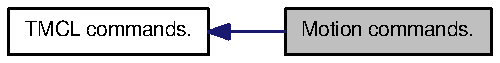
\includegraphics[width=138pt]{group__MotionComm}
\end{center}
\end{figure}
\subsection*{Defines}
\begin{DoxyCompactItemize}
\item 
\#define \hyperlink{group__MotionComm_gae60969d45c586023c9bd2db9498cc508}{TMCL\_\-ROR}~1
\item 
\#define \hyperlink{group__MotionComm_ga90f30df41b6fa29a3e94c909e655af94}{TMCL\_\-ROL}~2
\item 
\#define \hyperlink{group__MotionComm_ga94462741a6a5efcf6b175294cb9b6ecf}{TMCL\_\-MST}~3
\item 
\#define \hyperlink{group__MotionComm_ga109d51fee8df715b9e18b6c49b785757}{TMCL\_\-MVP}~4
\item 
\#define \hyperlink{group__MotionComm_ga316ddf99f164783c8488c48ce9346c21}{TMCL\_\-RFS}~13
\end{DoxyCompactItemize}


\subsection{Detailed Description}
Commands for controlling the motion of the module. 

\subsection{Define Documentation}
\hypertarget{group__MotionComm_ga94462741a6a5efcf6b175294cb9b6ecf}{
\index{MotionComm@{MotionComm}!TMCL\_\-MST@{TMCL\_\-MST}}
\index{TMCL\_\-MST@{TMCL\_\-MST}!MotionComm@{MotionComm}}
\subsubsection[{TMCL\_\-MST}]{\setlength{\rightskip}{0pt plus 5cm}\#define TMCL\_\-MST~3}}
\label{group__MotionComm_ga94462741a6a5efcf6b175294cb9b6ecf}
Motor stop 

Definition at line 79 of file tmcldefs.h.\hypertarget{group__MotionComm_ga109d51fee8df715b9e18b6c49b785757}{
\index{MotionComm@{MotionComm}!TMCL\_\-MVP@{TMCL\_\-MVP}}
\index{TMCL\_\-MVP@{TMCL\_\-MVP}!MotionComm@{MotionComm}}
\subsubsection[{TMCL\_\-MVP}]{\setlength{\rightskip}{0pt plus 5cm}\#define TMCL\_\-MVP~4}}
\label{group__MotionComm_ga109d51fee8df715b9e18b6c49b785757}
Move to position 

Definition at line 80 of file tmcldefs.h.\hypertarget{group__MotionComm_ga316ddf99f164783c8488c48ce9346c21}{
\index{MotionComm@{MotionComm}!TMCL\_\-RFS@{TMCL\_\-RFS}}
\index{TMCL\_\-RFS@{TMCL\_\-RFS}!MotionComm@{MotionComm}}
\subsubsection[{TMCL\_\-RFS}]{\setlength{\rightskip}{0pt plus 5cm}\#define TMCL\_\-RFS~13}}
\label{group__MotionComm_ga316ddf99f164783c8488c48ce9346c21}
Reference search 

Definition at line 81 of file tmcldefs.h.\hypertarget{group__MotionComm_ga90f30df41b6fa29a3e94c909e655af94}{
\index{MotionComm@{MotionComm}!TMCL\_\-ROL@{TMCL\_\-ROL}}
\index{TMCL\_\-ROL@{TMCL\_\-ROL}!MotionComm@{MotionComm}}
\subsubsection[{TMCL\_\-ROL}]{\setlength{\rightskip}{0pt plus 5cm}\#define TMCL\_\-ROL~2}}
\label{group__MotionComm_ga90f30df41b6fa29a3e94c909e655af94}
Rotate left 

Definition at line 78 of file tmcldefs.h.\hypertarget{group__MotionComm_gae60969d45c586023c9bd2db9498cc508}{
\index{MotionComm@{MotionComm}!TMCL\_\-ROR@{TMCL\_\-ROR}}
\index{TMCL\_\-ROR@{TMCL\_\-ROR}!MotionComm@{MotionComm}}
\subsubsection[{TMCL\_\-ROR}]{\setlength{\rightskip}{0pt plus 5cm}\#define TMCL\_\-ROR~1}}
\label{group__MotionComm_gae60969d45c586023c9bd2db9498cc508}
Rotate right 

Definition at line 77 of file tmcldefs.h.
\hypertarget{group__ParComm}{
\section{Parameter commands.}
\label{group__ParComm}\index{Parameter commands.@{Parameter commands.}}
}


Collaboration diagram for Parameter commands.:\nopagebreak
\begin{figure}[H]
\begin{center}
\leavevmode
\includegraphics[width=145pt]{group__ParComm}
\end{center}
\end{figure}
\subsection*{Defines}
\begin{DoxyCompactItemize}
\item 
\#define \hyperlink{group__ParComm_ga9d041a48b17f51e16e6219d3cfe5a2ca}{TMCL\_\-SAP}~5
\item 
\#define \hyperlink{group__ParComm_gaeac28ca289b13b735506291521646a4a}{TMCL\_\-GAP}~6
\item 
\#define \hyperlink{group__ParComm_ga22d01b4d2941ab2a2881f17975424f41}{TMCL\_\-STAP}~7
\item 
\#define \hyperlink{group__ParComm_gab338e76ee77e5f122d1694c728beb5e3}{TMCL\_\-RSAP}~8
\item 
\#define \hyperlink{group__ParComm_ga12919729038b159bb1f9b275c9c8f5bc}{TMCL\_\-SGP}~9
\item 
\#define \hyperlink{group__ParComm_ga4bf884d087a29a85073718bbd0d4f928}{TMCL\_\-GGP}~10
\item 
\#define \hyperlink{group__ParComm_ga209b905332339e2b52a7166f46ef2db9}{TMCL\_\-STGP}~11
\item 
\#define \hyperlink{group__ParComm_ga21517120fb13310ef4416fd370fa91b6}{TMCL\_\-RSGP}~12
\end{DoxyCompactItemize}


\subsection{Detailed Description}
Commands for setting module parameters. 

\subsection{Define Documentation}
\hypertarget{group__ParComm_gaeac28ca289b13b735506291521646a4a}{
\index{ParComm@{ParComm}!TMCL\_\-GAP@{TMCL\_\-GAP}}
\index{TMCL\_\-GAP@{TMCL\_\-GAP}!ParComm@{ParComm}}
\subsubsection[{TMCL\_\-GAP}]{\setlength{\rightskip}{0pt plus 5cm}\#define TMCL\_\-GAP~6}}
\label{group__ParComm_gaeac28ca289b13b735506291521646a4a}
Get Axis Parameter 

Definition at line 91 of file tmcldefs.h.\hypertarget{group__ParComm_ga4bf884d087a29a85073718bbd0d4f928}{
\index{ParComm@{ParComm}!TMCL\_\-GGP@{TMCL\_\-GGP}}
\index{TMCL\_\-GGP@{TMCL\_\-GGP}!ParComm@{ParComm}}
\subsubsection[{TMCL\_\-GGP}]{\setlength{\rightskip}{0pt plus 5cm}\#define TMCL\_\-GGP~10}}
\label{group__ParComm_ga4bf884d087a29a85073718bbd0d4f928}
Get Global Parameter 

Definition at line 95 of file tmcldefs.h.\hypertarget{group__ParComm_gab338e76ee77e5f122d1694c728beb5e3}{
\index{ParComm@{ParComm}!TMCL\_\-RSAP@{TMCL\_\-RSAP}}
\index{TMCL\_\-RSAP@{TMCL\_\-RSAP}!ParComm@{ParComm}}
\subsubsection[{TMCL\_\-RSAP}]{\setlength{\rightskip}{0pt plus 5cm}\#define TMCL\_\-RSAP~8}}
\label{group__ParComm_gab338e76ee77e5f122d1694c728beb5e3}
Restore Axis Parameter 

Definition at line 93 of file tmcldefs.h.\hypertarget{group__ParComm_ga21517120fb13310ef4416fd370fa91b6}{
\index{ParComm@{ParComm}!TMCL\_\-RSGP@{TMCL\_\-RSGP}}
\index{TMCL\_\-RSGP@{TMCL\_\-RSGP}!ParComm@{ParComm}}
\subsubsection[{TMCL\_\-RSGP}]{\setlength{\rightskip}{0pt plus 5cm}\#define TMCL\_\-RSGP~12}}
\label{group__ParComm_ga21517120fb13310ef4416fd370fa91b6}
Restore Global Parameter 

Definition at line 97 of file tmcldefs.h.\hypertarget{group__ParComm_ga9d041a48b17f51e16e6219d3cfe5a2ca}{
\index{ParComm@{ParComm}!TMCL\_\-SAP@{TMCL\_\-SAP}}
\index{TMCL\_\-SAP@{TMCL\_\-SAP}!ParComm@{ParComm}}
\subsubsection[{TMCL\_\-SAP}]{\setlength{\rightskip}{0pt plus 5cm}\#define TMCL\_\-SAP~5}}
\label{group__ParComm_ga9d041a48b17f51e16e6219d3cfe5a2ca}
Set Axis Parameter 

Definition at line 90 of file tmcldefs.h.\hypertarget{group__ParComm_ga12919729038b159bb1f9b275c9c8f5bc}{
\index{ParComm@{ParComm}!TMCL\_\-SGP@{TMCL\_\-SGP}}
\index{TMCL\_\-SGP@{TMCL\_\-SGP}!ParComm@{ParComm}}
\subsubsection[{TMCL\_\-SGP}]{\setlength{\rightskip}{0pt plus 5cm}\#define TMCL\_\-SGP~9}}
\label{group__ParComm_ga12919729038b159bb1f9b275c9c8f5bc}
Set Global Parameter 

Definition at line 94 of file tmcldefs.h.\hypertarget{group__ParComm_ga22d01b4d2941ab2a2881f17975424f41}{
\index{ParComm@{ParComm}!TMCL\_\-STAP@{TMCL\_\-STAP}}
\index{TMCL\_\-STAP@{TMCL\_\-STAP}!ParComm@{ParComm}}
\subsubsection[{TMCL\_\-STAP}]{\setlength{\rightskip}{0pt plus 5cm}\#define TMCL\_\-STAP~7}}
\label{group__ParComm_ga22d01b4d2941ab2a2881f17975424f41}
Store Axis Parameter 

Definition at line 92 of file tmcldefs.h.\hypertarget{group__ParComm_ga209b905332339e2b52a7166f46ef2db9}{
\index{ParComm@{ParComm}!TMCL\_\-STGP@{TMCL\_\-STGP}}
\index{TMCL\_\-STGP@{TMCL\_\-STGP}!ParComm@{ParComm}}
\subsubsection[{TMCL\_\-STGP}]{\setlength{\rightskip}{0pt plus 5cm}\#define TMCL\_\-STGP~11}}
\label{group__ParComm_ga209b905332339e2b52a7166f46ef2db9}
Store Global Parameter 

Definition at line 96 of file tmcldefs.h.
\hypertarget{group__CTLFuncs}{
\section{TMCL Control Functions}
\label{group__CTLFuncs}\index{TMCL Control Functions@{TMCL Control Functions}}
}


Collaboration diagram for TMCL Control Functions:\nopagebreak
\begin{figure}[H]
\begin{center}
\leavevmode
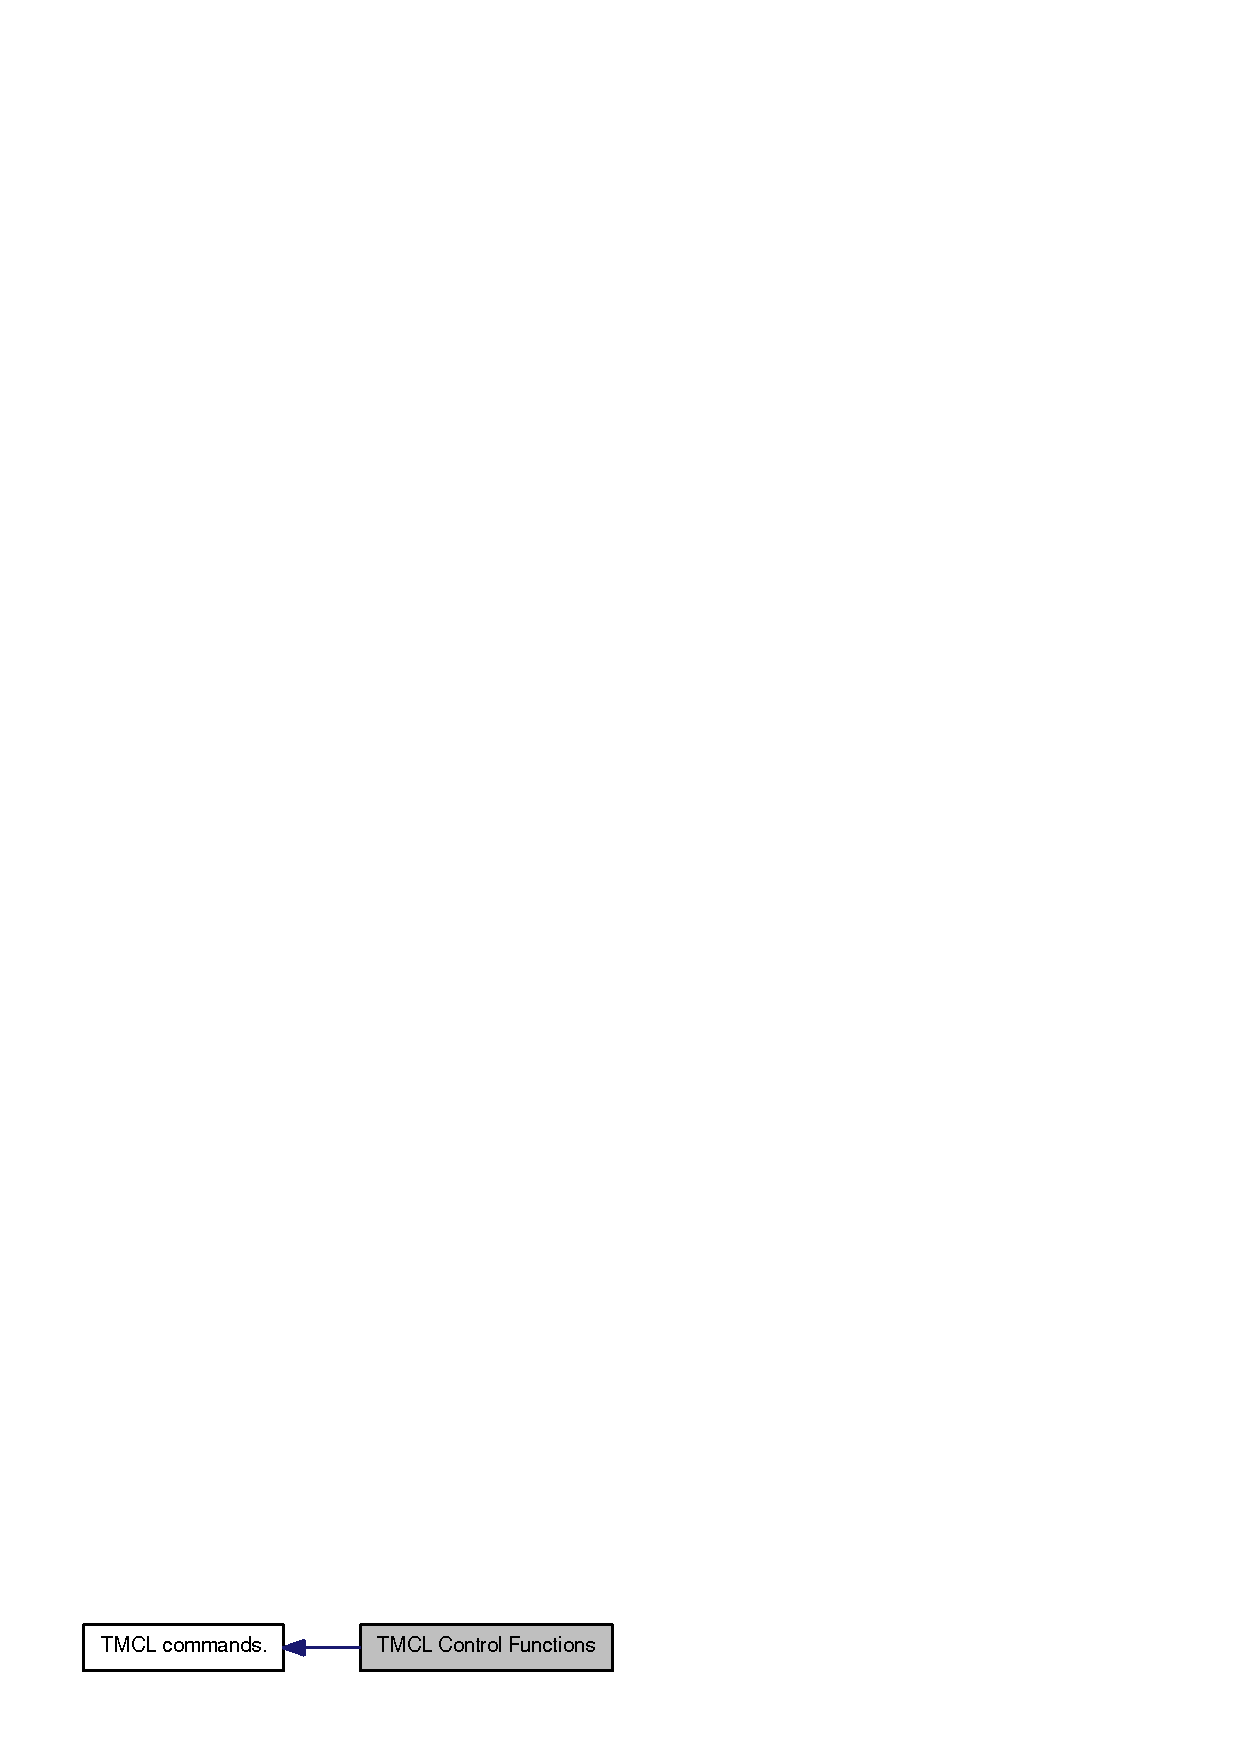
\includegraphics[width=149pt]{group__CTLFuncs}
\end{center}
\end{figure}
\subsection*{Defines}
\begin{DoxyCompactItemize}
\item 
\#define \hyperlink{group__CTLFuncs_gaa9e1148b7664ea0b5a78f845332b4fd7}{TMCL\_\-CTL\_\-STOP}~128
\item 
\#define \hyperlink{group__CTLFuncs_ga22166cf0f91912ea37048297d8030247}{TMCL\_\-CTL\_\-RUN}~129
\item 
\#define \hyperlink{group__CTLFuncs_ga0ffb8262b5b83a477e839844789fe986}{TMCL\_\-CTL\_\-STEP}~130
\item 
\#define \hyperlink{group__CTLFuncs_ga433f27b92ba499465f7eab488fbd3cea}{TMCL\_\-CTL\_\-RST}~131
\item 
\#define \hyperlink{group__CTLFuncs_gab0ffec97bdd896d0d98eacf2c80ac946}{TMCL\_\-CTL\_\-DLM\_\-START}~132
\item 
\#define \hyperlink{group__CTLFuncs_gaff3c81037366905174f34c8406f058c7}{TMCL\_\-CTL\_\-DLM\_\-QUIT}~133
\item 
\#define \hyperlink{group__CTLFuncs_ga9d883e9bae5236c285877f884bb8a613}{TMCL\_\-CTL\_\-READMEM}~134
\item 
\#define \hyperlink{group__CTLFuncs_gaf8364761b483fed9c95abaedffcf0ec2}{TMCL\_\-CTL\_\-STATUS}~135
\item 
\#define \hyperlink{group__CTLFuncs_gaac0228cc9a707b904b510de74a7fb505}{TMCL\_\-CTL\_\-FW\_\-VER}~136
\item 
\#define \hyperlink{group__CTLFuncs_gab41e9c01de441b30b228801e51243895}{TMCL\_\-CTL\_\-FACTORY}~137
\item 
\#define \hyperlink{group__CTLFuncs_ga36f62eadca8ba64c832ac6120f5a372a}{TMCL\_\-CTL\_\-ASCII}~139
\end{DoxyCompactItemize}


\subsection{Detailed Description}
Commands for controlling the TMCL module.

\begin{DoxyNote}{Note}
{\itshape Not to be used in stand-\/alone mode\/} 
\end{DoxyNote}


\subsection{Define Documentation}
\hypertarget{group__CTLFuncs_ga36f62eadca8ba64c832ac6120f5a372a}{
\index{CTLFuncs@{CTLFuncs}!TMCL\_\-CTL\_\-ASCII@{TMCL\_\-CTL\_\-ASCII}}
\index{TMCL\_\-CTL\_\-ASCII@{TMCL\_\-CTL\_\-ASCII}!CTLFuncs@{CTLFuncs}}
\subsubsection[{TMCL\_\-CTL\_\-ASCII}]{\setlength{\rightskip}{0pt plus 5cm}\#define TMCL\_\-CTL\_\-ASCII~139}}
\label{group__CTLFuncs_ga36f62eadca8ba64c832ac6120f5a372a}
Enter ASCII mode 

Definition at line 147 of file tmcldefs.h.\hypertarget{group__CTLFuncs_gaff3c81037366905174f34c8406f058c7}{
\index{CTLFuncs@{CTLFuncs}!TMCL\_\-CTL\_\-DLM\_\-QUIT@{TMCL\_\-CTL\_\-DLM\_\-QUIT}}
\index{TMCL\_\-CTL\_\-DLM\_\-QUIT@{TMCL\_\-CTL\_\-DLM\_\-QUIT}!CTLFuncs@{CTLFuncs}}
\subsubsection[{TMCL\_\-CTL\_\-DLM\_\-QUIT}]{\setlength{\rightskip}{0pt plus 5cm}\#define TMCL\_\-CTL\_\-DLM\_\-QUIT~133}}
\label{group__CTLFuncs_gaff3c81037366905174f34c8406f058c7}
Stop download mode 

Definition at line 141 of file tmcldefs.h.\hypertarget{group__CTLFuncs_gab0ffec97bdd896d0d98eacf2c80ac946}{
\index{CTLFuncs@{CTLFuncs}!TMCL\_\-CTL\_\-DLM\_\-START@{TMCL\_\-CTL\_\-DLM\_\-START}}
\index{TMCL\_\-CTL\_\-DLM\_\-START@{TMCL\_\-CTL\_\-DLM\_\-START}!CTLFuncs@{CTLFuncs}}
\subsubsection[{TMCL\_\-CTL\_\-DLM\_\-START}]{\setlength{\rightskip}{0pt plus 5cm}\#define TMCL\_\-CTL\_\-DLM\_\-START~132}}
\label{group__CTLFuncs_gab0ffec97bdd896d0d98eacf2c80ac946}
Start download mode 

Definition at line 140 of file tmcldefs.h.\hypertarget{group__CTLFuncs_gab41e9c01de441b30b228801e51243895}{
\index{CTLFuncs@{CTLFuncs}!TMCL\_\-CTL\_\-FACTORY@{TMCL\_\-CTL\_\-FACTORY}}
\index{TMCL\_\-CTL\_\-FACTORY@{TMCL\_\-CTL\_\-FACTORY}!CTLFuncs@{CTLFuncs}}
\subsubsection[{TMCL\_\-CTL\_\-FACTORY}]{\setlength{\rightskip}{0pt plus 5cm}\#define TMCL\_\-CTL\_\-FACTORY~137}}
\label{group__CTLFuncs_gab41e9c01de441b30b228801e51243895}
Restore factory settings 

Definition at line 145 of file tmcldefs.h.\hypertarget{group__CTLFuncs_gaac0228cc9a707b904b510de74a7fb505}{
\index{CTLFuncs@{CTLFuncs}!TMCL\_\-CTL\_\-FW\_\-VER@{TMCL\_\-CTL\_\-FW\_\-VER}}
\index{TMCL\_\-CTL\_\-FW\_\-VER@{TMCL\_\-CTL\_\-FW\_\-VER}!CTLFuncs@{CTLFuncs}}
\subsubsection[{TMCL\_\-CTL\_\-FW\_\-VER}]{\setlength{\rightskip}{0pt plus 5cm}\#define TMCL\_\-CTL\_\-FW\_\-VER~136}}
\label{group__CTLFuncs_gaac0228cc9a707b904b510de74a7fb505}
Get firmware version 

Definition at line 144 of file tmcldefs.h.\hypertarget{group__CTLFuncs_ga9d883e9bae5236c285877f884bb8a613}{
\index{CTLFuncs@{CTLFuncs}!TMCL\_\-CTL\_\-READMEM@{TMCL\_\-CTL\_\-READMEM}}
\index{TMCL\_\-CTL\_\-READMEM@{TMCL\_\-CTL\_\-READMEM}!CTLFuncs@{CTLFuncs}}
\subsubsection[{TMCL\_\-CTL\_\-READMEM}]{\setlength{\rightskip}{0pt plus 5cm}\#define TMCL\_\-CTL\_\-READMEM~134}}
\label{group__CTLFuncs_ga9d883e9bae5236c285877f884bb8a613}
Read TMCL memory 

Definition at line 142 of file tmcldefs.h.\hypertarget{group__CTLFuncs_ga433f27b92ba499465f7eab488fbd3cea}{
\index{CTLFuncs@{CTLFuncs}!TMCL\_\-CTL\_\-RST@{TMCL\_\-CTL\_\-RST}}
\index{TMCL\_\-CTL\_\-RST@{TMCL\_\-CTL\_\-RST}!CTLFuncs@{CTLFuncs}}
\subsubsection[{TMCL\_\-CTL\_\-RST}]{\setlength{\rightskip}{0pt plus 5cm}\#define TMCL\_\-CTL\_\-RST~131}}
\label{group__CTLFuncs_ga433f27b92ba499465f7eab488fbd3cea}
Reset application 

Definition at line 139 of file tmcldefs.h.\hypertarget{group__CTLFuncs_ga22166cf0f91912ea37048297d8030247}{
\index{CTLFuncs@{CTLFuncs}!TMCL\_\-CTL\_\-RUN@{TMCL\_\-CTL\_\-RUN}}
\index{TMCL\_\-CTL\_\-RUN@{TMCL\_\-CTL\_\-RUN}!CTLFuncs@{CTLFuncs}}
\subsubsection[{TMCL\_\-CTL\_\-RUN}]{\setlength{\rightskip}{0pt plus 5cm}\#define TMCL\_\-CTL\_\-RUN~129}}
\label{group__CTLFuncs_ga22166cf0f91912ea37048297d8030247}
Run application 

Definition at line 137 of file tmcldefs.h.\hypertarget{group__CTLFuncs_gaf8364761b483fed9c95abaedffcf0ec2}{
\index{CTLFuncs@{CTLFuncs}!TMCL\_\-CTL\_\-STATUS@{TMCL\_\-CTL\_\-STATUS}}
\index{TMCL\_\-CTL\_\-STATUS@{TMCL\_\-CTL\_\-STATUS}!CTLFuncs@{CTLFuncs}}
\subsubsection[{TMCL\_\-CTL\_\-STATUS}]{\setlength{\rightskip}{0pt plus 5cm}\#define TMCL\_\-CTL\_\-STATUS~135}}
\label{group__CTLFuncs_gaf8364761b483fed9c95abaedffcf0ec2}
Get application status 

Definition at line 143 of file tmcldefs.h.\hypertarget{group__CTLFuncs_ga0ffb8262b5b83a477e839844789fe986}{
\index{CTLFuncs@{CTLFuncs}!TMCL\_\-CTL\_\-STEP@{TMCL\_\-CTL\_\-STEP}}
\index{TMCL\_\-CTL\_\-STEP@{TMCL\_\-CTL\_\-STEP}!CTLFuncs@{CTLFuncs}}
\subsubsection[{TMCL\_\-CTL\_\-STEP}]{\setlength{\rightskip}{0pt plus 5cm}\#define TMCL\_\-CTL\_\-STEP~130}}
\label{group__CTLFuncs_ga0ffb8262b5b83a477e839844789fe986}
Only exectute next command of application 

Definition at line 138 of file tmcldefs.h.\hypertarget{group__CTLFuncs_gaa9e1148b7664ea0b5a78f845332b4fd7}{
\index{CTLFuncs@{CTLFuncs}!TMCL\_\-CTL\_\-STOP@{TMCL\_\-CTL\_\-STOP}}
\index{TMCL\_\-CTL\_\-STOP@{TMCL\_\-CTL\_\-STOP}!CTLFuncs@{CTLFuncs}}
\subsubsection[{TMCL\_\-CTL\_\-STOP}]{\setlength{\rightskip}{0pt plus 5cm}\#define TMCL\_\-CTL\_\-STOP~128}}
\label{group__CTLFuncs_gaa9e1148b7664ea0b5a78f845332b4fd7}
Stop application 

Definition at line 136 of file tmcldefs.h.
\hypertarget{group__TypeCodes}{
\section{TMCL operation type codes.}
\label{group__TypeCodes}\index{TMCL operation type codes.@{TMCL operation type codes.}}
}


Collaboration diagram for TMCL operation type codes.:\nopagebreak
\begin{figure}[H]
\begin{center}
\leavevmode
\includegraphics[width=158pt]{group__TypeCodes}
\end{center}
\end{figure}
Operation type codes for TMCL commands. 
\hypertarget{group__AxisParam}{
\section{Axis Parameters}
\label{group__AxisParam}\index{Axis Parameters@{Axis Parameters}}
}


Collaboration diagram for Axis Parameters:\nopagebreak
\begin{figure}[H]
\begin{center}
\leavevmode
\includegraphics[width=142pt]{group__AxisParam}
\end{center}
\end{figure}
\subsection*{Modules}
\begin{DoxyCompactItemize}
\item 
\hyperlink{group__RWParam}{Read-\/Write Parameters}
\item 
\hyperlink{group__ROParam}{Read-\/Only Parameters}
\end{DoxyCompactItemize}


\subsection{Detailed Description}
Axis parameters to be used with TMCL\_\-SAP, TMCL\_\-GAP, TMCL\_\-AAP, TMCL\_\-STAP and TMCL\_\-RSAP for TMCM-\/3xx/11x/109/61x modules.

\begin{Desc}
\item[\hyperlink{todo__todo000004}{Todo}]These are not complete. \end{Desc}

\hypertarget{group__RWParam}{
\section{Read-\/Write Parameters}
\label{group__RWParam}\index{Read-\/Write Parameters@{Read-\/Write Parameters}}
}


Collaboration diagram for Read-\/Write Parameters:\nopagebreak
\begin{figure}[H]
\begin{center}
\leavevmode
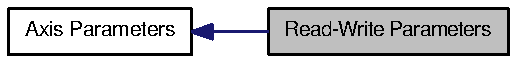
\includegraphics[width=142pt]{group__RWParam}
\end{center}
\end{figure}
\subsection*{Defines}
\begin{DoxyCompactItemize}
\item 
\#define \hyperlink{group__RWParam_ga87dfb3db656c898683ae4a5dd80e789a}{TMCL\_\-AP\_\-TARGET\_\-POS}~0
\item 
\#define \hyperlink{group__RWParam_ga46ffdf772b16b88c99f5b48893b3f710}{TMCL\_\-AP\_\-CURR\_\-POS}~1
\item 
\#define \hyperlink{group__RWParam_ga9f34f155a65163069922f5f20c4c63b5}{TMCL\_\-AP\_\-TARGET\_\-SPEED}~2
\item 
\#define \hyperlink{group__RWParam_gafeecf0d7ec4c89beea4eb6e5dd3d5326}{TMCL\_\-AP\_\-MAX\_\-POS\_\-SPEED}~4
\item 
\#define \hyperlink{group__RWParam_ga5f18e570598b33d3d77b0d0894d81dc7}{TMCL\_\-AP\_\-MAX\_\-ACCEL}~5
\item 
\#define \hyperlink{group__RWParam_gaaf8d5010f2cf9799b5321358b5f5fb35}{TMCL\_\-AP\_\-ABS\_\-CURRENT}~6
\item 
\#define \hyperlink{group__RWParam_ga7e4a74f86decbbced917fb7825aef450}{TMCL\_\-AP\_\-STBY\_\-CURRENT}~7
\item 
\#define \hyperlink{group__RWParam_ga126f3a0bebd82760451aeadab91d6e06}{TMCL\_\-AP\_\-DISABLE\_\-LIMIT\_\-R}~12
\item 
\#define \hyperlink{group__RWParam_ga36067071d35368d2a1b03ddfae1d4eb9}{TMCL\_\-AP\_\-DISABLE\_\-LIMIT\_\-L}~13
\item 
\#define \hyperlink{group__RWParam_gab96353fcd1f433ef38ea445f812d2616}{TMCL\_\-AP\_\-SR\_\-PRESC}~14
\item 
\#define \hyperlink{group__RWParam_gaaf9500c37e13a506bcebb07378bb559c}{TMCL\_\-AP\_\-MICROSTEPS}~140
\item 
\#define \hyperlink{group__RWParam_ga6c4829576ea5ead497c9fd6bc564ecf0}{TMCL\_\-AP\_\-MAX\_\-CURR\_\-REST}~143
\item 
\#define \hyperlink{group__RWParam_gad989938d2101b5e000d5f41ca1d2a522}{TMCL\_\-AP\_\-MAX\_\-CURR\_\-LOW\_\-ACCEL}~144
\item 
\#define \hyperlink{group__RWParam_ga1a3faf0da53cb9d7cc2a84cc326ccc4a}{TMCL\_\-AP\_\-MAX\_\-CURR\_\-HIGH\_\-ACCEL}~145
\item 
\#define \hyperlink{group__RWParam_gaf504e536f23e990387a1b4421fcc49e4}{TMCL\_\-AP\_\-RFS\_\-MODE}~193
\item 
\#define \hyperlink{group__RWParam_ga4c6ebda674b3ce393db587761c169515}{TMCL\_\-AP\_\-RFS\_\-SPEED}~194
\item 
\#define \hyperlink{group__RWParam_ga31404aaf7195272cd4a6ef150d6ea421}{TMCL\_\-AP\_\-RFS\_\-SW\_\-SPEED}~195
\end{DoxyCompactItemize}


\subsection{Detailed Description}
Parameters that can be read and written 

\subsection{Define Documentation}
\hypertarget{group__RWParam_gaaf8d5010f2cf9799b5321358b5f5fb35}{
\index{RWParam@{RWParam}!TMCL\_\-AP\_\-ABS\_\-CURRENT@{TMCL\_\-AP\_\-ABS\_\-CURRENT}}
\index{TMCL\_\-AP\_\-ABS\_\-CURRENT@{TMCL\_\-AP\_\-ABS\_\-CURRENT}!RWParam@{RWParam}}
\subsubsection[{TMCL\_\-AP\_\-ABS\_\-CURRENT}]{\setlength{\rightskip}{0pt plus 5cm}\#define TMCL\_\-AP\_\-ABS\_\-CURRENT~6}}
\label{group__RWParam_gaaf8d5010f2cf9799b5321358b5f5fb35}
Maximum absolute current 

Definition at line 187 of file tmcldefs.h.\hypertarget{group__RWParam_ga46ffdf772b16b88c99f5b48893b3f710}{
\index{RWParam@{RWParam}!TMCL\_\-AP\_\-CURR\_\-POS@{TMCL\_\-AP\_\-CURR\_\-POS}}
\index{TMCL\_\-AP\_\-CURR\_\-POS@{TMCL\_\-AP\_\-CURR\_\-POS}!RWParam@{RWParam}}
\subsubsection[{TMCL\_\-AP\_\-CURR\_\-POS}]{\setlength{\rightskip}{0pt plus 5cm}\#define TMCL\_\-AP\_\-CURR\_\-POS~1}}
\label{group__RWParam_ga46ffdf772b16b88c99f5b48893b3f710}
Current position 

Definition at line 183 of file tmcldefs.h.\hypertarget{group__RWParam_ga36067071d35368d2a1b03ddfae1d4eb9}{
\index{RWParam@{RWParam}!TMCL\_\-AP\_\-DISABLE\_\-LIMIT\_\-L@{TMCL\_\-AP\_\-DISABLE\_\-LIMIT\_\-L}}
\index{TMCL\_\-AP\_\-DISABLE\_\-LIMIT\_\-L@{TMCL\_\-AP\_\-DISABLE\_\-LIMIT\_\-L}!RWParam@{RWParam}}
\subsubsection[{TMCL\_\-AP\_\-DISABLE\_\-LIMIT\_\-L}]{\setlength{\rightskip}{0pt plus 5cm}\#define TMCL\_\-AP\_\-DISABLE\_\-LIMIT\_\-L~13}}
\label{group__RWParam_ga36067071d35368d2a1b03ddfae1d4eb9}
Disable the left limit switch 

Definition at line 190 of file tmcldefs.h.\hypertarget{group__RWParam_ga126f3a0bebd82760451aeadab91d6e06}{
\index{RWParam@{RWParam}!TMCL\_\-AP\_\-DISABLE\_\-LIMIT\_\-R@{TMCL\_\-AP\_\-DISABLE\_\-LIMIT\_\-R}}
\index{TMCL\_\-AP\_\-DISABLE\_\-LIMIT\_\-R@{TMCL\_\-AP\_\-DISABLE\_\-LIMIT\_\-R}!RWParam@{RWParam}}
\subsubsection[{TMCL\_\-AP\_\-DISABLE\_\-LIMIT\_\-R}]{\setlength{\rightskip}{0pt plus 5cm}\#define TMCL\_\-AP\_\-DISABLE\_\-LIMIT\_\-R~12}}
\label{group__RWParam_ga126f3a0bebd82760451aeadab91d6e06}
Disable the right limit switch 

Definition at line 189 of file tmcldefs.h.\hypertarget{group__RWParam_ga5f18e570598b33d3d77b0d0894d81dc7}{
\index{RWParam@{RWParam}!TMCL\_\-AP\_\-MAX\_\-ACCEL@{TMCL\_\-AP\_\-MAX\_\-ACCEL}}
\index{TMCL\_\-AP\_\-MAX\_\-ACCEL@{TMCL\_\-AP\_\-MAX\_\-ACCEL}!RWParam@{RWParam}}
\subsubsection[{TMCL\_\-AP\_\-MAX\_\-ACCEL}]{\setlength{\rightskip}{0pt plus 5cm}\#define TMCL\_\-AP\_\-MAX\_\-ACCEL~5}}
\label{group__RWParam_ga5f18e570598b33d3d77b0d0894d81dc7}
Maximum acceleration 

Definition at line 186 of file tmcldefs.h.\hypertarget{group__RWParam_ga1a3faf0da53cb9d7cc2a84cc326ccc4a}{
\index{RWParam@{RWParam}!TMCL\_\-AP\_\-MAX\_\-CURR\_\-HIGH\_\-ACCEL@{TMCL\_\-AP\_\-MAX\_\-CURR\_\-HIGH\_\-ACCEL}}
\index{TMCL\_\-AP\_\-MAX\_\-CURR\_\-HIGH\_\-ACCEL@{TMCL\_\-AP\_\-MAX\_\-CURR\_\-HIGH\_\-ACCEL}!RWParam@{RWParam}}
\subsubsection[{TMCL\_\-AP\_\-MAX\_\-CURR\_\-HIGH\_\-ACCEL}]{\setlength{\rightskip}{0pt plus 5cm}\#define TMCL\_\-AP\_\-MAX\_\-CURR\_\-HIGH\_\-ACCEL~145}}
\label{group__RWParam_ga1a3faf0da53cb9d7cc2a84cc326ccc4a}
Maximal current at high acceleration (Normally use \hyperlink{group__RWParam_gaaf8d5010f2cf9799b5321358b5f5fb35}{TMCL\_\-AP\_\-ABS\_\-CURRENT} and \hyperlink{group__RWParam_ga7e4a74f86decbbced917fb7825aef450}{TMCL\_\-AP\_\-STBY\_\-CURRENT}) 

Definition at line 198 of file tmcldefs.h.\hypertarget{group__RWParam_gad989938d2101b5e000d5f41ca1d2a522}{
\index{RWParam@{RWParam}!TMCL\_\-AP\_\-MAX\_\-CURR\_\-LOW\_\-ACCEL@{TMCL\_\-AP\_\-MAX\_\-CURR\_\-LOW\_\-ACCEL}}
\index{TMCL\_\-AP\_\-MAX\_\-CURR\_\-LOW\_\-ACCEL@{TMCL\_\-AP\_\-MAX\_\-CURR\_\-LOW\_\-ACCEL}!RWParam@{RWParam}}
\subsubsection[{TMCL\_\-AP\_\-MAX\_\-CURR\_\-LOW\_\-ACCEL}]{\setlength{\rightskip}{0pt plus 5cm}\#define TMCL\_\-AP\_\-MAX\_\-CURR\_\-LOW\_\-ACCEL~144}}
\label{group__RWParam_gad989938d2101b5e000d5f41ca1d2a522}
Maximal current at low acceleration (Normally use \hyperlink{group__RWParam_gaaf8d5010f2cf9799b5321358b5f5fb35}{TMCL\_\-AP\_\-ABS\_\-CURRENT} and \hyperlink{group__RWParam_ga7e4a74f86decbbced917fb7825aef450}{TMCL\_\-AP\_\-STBY\_\-CURRENT}) 

Definition at line 197 of file tmcldefs.h.\hypertarget{group__RWParam_ga6c4829576ea5ead497c9fd6bc564ecf0}{
\index{RWParam@{RWParam}!TMCL\_\-AP\_\-MAX\_\-CURR\_\-REST@{TMCL\_\-AP\_\-MAX\_\-CURR\_\-REST}}
\index{TMCL\_\-AP\_\-MAX\_\-CURR\_\-REST@{TMCL\_\-AP\_\-MAX\_\-CURR\_\-REST}!RWParam@{RWParam}}
\subsubsection[{TMCL\_\-AP\_\-MAX\_\-CURR\_\-REST}]{\setlength{\rightskip}{0pt plus 5cm}\#define TMCL\_\-AP\_\-MAX\_\-CURR\_\-REST~143}}
\label{group__RWParam_ga6c4829576ea5ead497c9fd6bc564ecf0}
Maximal current at rest (Normally use \hyperlink{group__RWParam_gaaf8d5010f2cf9799b5321358b5f5fb35}{TMCL\_\-AP\_\-ABS\_\-CURRENT} and \hyperlink{group__RWParam_ga7e4a74f86decbbced917fb7825aef450}{TMCL\_\-AP\_\-STBY\_\-CURRENT}) 

Definition at line 196 of file tmcldefs.h.\hypertarget{group__RWParam_gafeecf0d7ec4c89beea4eb6e5dd3d5326}{
\index{RWParam@{RWParam}!TMCL\_\-AP\_\-MAX\_\-POS\_\-SPEED@{TMCL\_\-AP\_\-MAX\_\-POS\_\-SPEED}}
\index{TMCL\_\-AP\_\-MAX\_\-POS\_\-SPEED@{TMCL\_\-AP\_\-MAX\_\-POS\_\-SPEED}!RWParam@{RWParam}}
\subsubsection[{TMCL\_\-AP\_\-MAX\_\-POS\_\-SPEED}]{\setlength{\rightskip}{0pt plus 5cm}\#define TMCL\_\-AP\_\-MAX\_\-POS\_\-SPEED~4}}
\label{group__RWParam_gafeecf0d7ec4c89beea4eb6e5dd3d5326}
Maximum positioning speed 

Definition at line 185 of file tmcldefs.h.\hypertarget{group__RWParam_gaaf9500c37e13a506bcebb07378bb559c}{
\index{RWParam@{RWParam}!TMCL\_\-AP\_\-MICROSTEPS@{TMCL\_\-AP\_\-MICROSTEPS}}
\index{TMCL\_\-AP\_\-MICROSTEPS@{TMCL\_\-AP\_\-MICROSTEPS}!RWParam@{RWParam}}
\subsubsection[{TMCL\_\-AP\_\-MICROSTEPS}]{\setlength{\rightskip}{0pt plus 5cm}\#define TMCL\_\-AP\_\-MICROSTEPS~140}}
\label{group__RWParam_gaaf9500c37e13a506bcebb07378bb559c}
Extended Parameters Microstep mode (\begin{DoxySeeAlso}{See also}
TMCLMicrosteps) 
\end{DoxySeeAlso}


Definition at line 195 of file tmcldefs.h.\hypertarget{group__RWParam_gaf504e536f23e990387a1b4421fcc49e4}{
\index{RWParam@{RWParam}!TMCL\_\-AP\_\-RFS\_\-MODE@{TMCL\_\-AP\_\-RFS\_\-MODE}}
\index{TMCL\_\-AP\_\-RFS\_\-MODE@{TMCL\_\-AP\_\-RFS\_\-MODE}!RWParam@{RWParam}}
\subsubsection[{TMCL\_\-AP\_\-RFS\_\-MODE}]{\setlength{\rightskip}{0pt plus 5cm}\#define TMCL\_\-AP\_\-RFS\_\-MODE~193}}
\label{group__RWParam_gaf504e536f23e990387a1b4421fcc49e4}
Reference search mode 

Definition at line 199 of file tmcldefs.h.\hypertarget{group__RWParam_ga4c6ebda674b3ce393db587761c169515}{
\index{RWParam@{RWParam}!TMCL\_\-AP\_\-RFS\_\-SPEED@{TMCL\_\-AP\_\-RFS\_\-SPEED}}
\index{TMCL\_\-AP\_\-RFS\_\-SPEED@{TMCL\_\-AP\_\-RFS\_\-SPEED}!RWParam@{RWParam}}
\subsubsection[{TMCL\_\-AP\_\-RFS\_\-SPEED}]{\setlength{\rightskip}{0pt plus 5cm}\#define TMCL\_\-AP\_\-RFS\_\-SPEED~194}}
\label{group__RWParam_ga4c6ebda674b3ce393db587761c169515}
Reference search speed mode 

Definition at line 200 of file tmcldefs.h.\hypertarget{group__RWParam_ga31404aaf7195272cd4a6ef150d6ea421}{
\index{RWParam@{RWParam}!TMCL\_\-AP\_\-RFS\_\-SW\_\-SPEED@{TMCL\_\-AP\_\-RFS\_\-SW\_\-SPEED}}
\index{TMCL\_\-AP\_\-RFS\_\-SW\_\-SPEED@{TMCL\_\-AP\_\-RFS\_\-SW\_\-SPEED}!RWParam@{RWParam}}
\subsubsection[{TMCL\_\-AP\_\-RFS\_\-SW\_\-SPEED}]{\setlength{\rightskip}{0pt plus 5cm}\#define TMCL\_\-AP\_\-RFS\_\-SW\_\-SPEED~195}}
\label{group__RWParam_ga31404aaf7195272cd4a6ef150d6ea421}
Reference search speed at switch position 

Definition at line 201 of file tmcldefs.h.\hypertarget{group__RWParam_gab96353fcd1f433ef38ea445f812d2616}{
\index{RWParam@{RWParam}!TMCL\_\-AP\_\-SR\_\-PRESC@{TMCL\_\-AP\_\-SR\_\-PRESC}}
\index{TMCL\_\-AP\_\-SR\_\-PRESC@{TMCL\_\-AP\_\-SR\_\-PRESC}!RWParam@{RWParam}}
\subsubsection[{TMCL\_\-AP\_\-SR\_\-PRESC}]{\setlength{\rightskip}{0pt plus 5cm}\#define TMCL\_\-AP\_\-SR\_\-PRESC~14}}
\label{group__RWParam_gab96353fcd1f433ef38ea445f812d2616}
\begin{DoxyNote}{Note}
Currently not used 
\end{DoxyNote}


Definition at line 191 of file tmcldefs.h.\hypertarget{group__RWParam_ga7e4a74f86decbbced917fb7825aef450}{
\index{RWParam@{RWParam}!TMCL\_\-AP\_\-STBY\_\-CURRENT@{TMCL\_\-AP\_\-STBY\_\-CURRENT}}
\index{TMCL\_\-AP\_\-STBY\_\-CURRENT@{TMCL\_\-AP\_\-STBY\_\-CURRENT}!RWParam@{RWParam}}
\subsubsection[{TMCL\_\-AP\_\-STBY\_\-CURRENT}]{\setlength{\rightskip}{0pt plus 5cm}\#define TMCL\_\-AP\_\-STBY\_\-CURRENT~7}}
\label{group__RWParam_ga7e4a74f86decbbced917fb7825aef450}
Maximum standby current 

Definition at line 188 of file tmcldefs.h.\hypertarget{group__RWParam_ga87dfb3db656c898683ae4a5dd80e789a}{
\index{RWParam@{RWParam}!TMCL\_\-AP\_\-TARGET\_\-POS@{TMCL\_\-AP\_\-TARGET\_\-POS}}
\index{TMCL\_\-AP\_\-TARGET\_\-POS@{TMCL\_\-AP\_\-TARGET\_\-POS}!RWParam@{RWParam}}
\subsubsection[{TMCL\_\-AP\_\-TARGET\_\-POS}]{\setlength{\rightskip}{0pt plus 5cm}\#define TMCL\_\-AP\_\-TARGET\_\-POS~0}}
\label{group__RWParam_ga87dfb3db656c898683ae4a5dd80e789a}
Basic parameters Target (next) postition 

Definition at line 182 of file tmcldefs.h.\hypertarget{group__RWParam_ga9f34f155a65163069922f5f20c4c63b5}{
\index{RWParam@{RWParam}!TMCL\_\-AP\_\-TARGET\_\-SPEED@{TMCL\_\-AP\_\-TARGET\_\-SPEED}}
\index{TMCL\_\-AP\_\-TARGET\_\-SPEED@{TMCL\_\-AP\_\-TARGET\_\-SPEED}!RWParam@{RWParam}}
\subsubsection[{TMCL\_\-AP\_\-TARGET\_\-SPEED}]{\setlength{\rightskip}{0pt plus 5cm}\#define TMCL\_\-AP\_\-TARGET\_\-SPEED~2}}
\label{group__RWParam_ga9f34f155a65163069922f5f20c4c63b5}
Desired speed in velocity mode 

Definition at line 184 of file tmcldefs.h.
\hypertarget{group__ROParam}{
\section{Read-\/Only Parameters}
\label{group__ROParam}\index{Read-\/Only Parameters@{Read-\/Only Parameters}}
}


Collaboration diagram for Read-\/Only Parameters:\nopagebreak
\begin{figure}[H]
\begin{center}
\leavevmode
\includegraphics[width=141pt]{group__ROParam}
\end{center}
\end{figure}
\subsection*{Defines}
\begin{DoxyCompactItemize}
\item 
\#define \hyperlink{group__ROParam_ga3473b35e8f38849da91e101a751b474d}{TMCL\_\-AP\_\-CURR\_\-SPEED}~3
\item 
\#define \hyperlink{group__ROParam_ga8340c6753a1858eae01d9a7a0f1ea221}{TMCL\_\-AP\_\-POS\_\-REACHED}~8
\item 
\#define \hyperlink{group__ROParam_ga389a6e3b6ba6e1bc1ad719f055bf139f}{TMCL\_\-AP\_\-LIMIT\_\-R}~9
\item 
\#define \hyperlink{group__ROParam_ga4751b3398d03d02e756d6b564a735b51}{TMCL\_\-AP\_\-LIMIT\_\-L}~10
\end{DoxyCompactItemize}


\subsection{Detailed Description}
196 and 197 reserved

Parameters that can only be read 

\subsection{Define Documentation}
\hypertarget{group__ROParam_ga3473b35e8f38849da91e101a751b474d}{
\index{ROParam@{ROParam}!TMCL\_\-AP\_\-CURR\_\-SPEED@{TMCL\_\-AP\_\-CURR\_\-SPEED}}
\index{TMCL\_\-AP\_\-CURR\_\-SPEED@{TMCL\_\-AP\_\-CURR\_\-SPEED}!ROParam@{ROParam}}
\subsubsection[{TMCL\_\-AP\_\-CURR\_\-SPEED}]{\setlength{\rightskip}{0pt plus 5cm}\#define TMCL\_\-AP\_\-CURR\_\-SPEED~3}}
\label{group__ROParam_ga3473b35e8f38849da91e101a751b474d}
Basic parameters Current speed 

Definition at line 212 of file tmcldefs.h.\hypertarget{group__ROParam_ga4751b3398d03d02e756d6b564a735b51}{
\index{ROParam@{ROParam}!TMCL\_\-AP\_\-LIMIT\_\-L@{TMCL\_\-AP\_\-LIMIT\_\-L}}
\index{TMCL\_\-AP\_\-LIMIT\_\-L@{TMCL\_\-AP\_\-LIMIT\_\-L}!ROParam@{ROParam}}
\subsubsection[{TMCL\_\-AP\_\-LIMIT\_\-L}]{\setlength{\rightskip}{0pt plus 5cm}\#define TMCL\_\-AP\_\-LIMIT\_\-L~10}}
\label{group__ROParam_ga4751b3398d03d02e756d6b564a735b51}
Left limit switch status 

Definition at line 215 of file tmcldefs.h.\hypertarget{group__ROParam_ga389a6e3b6ba6e1bc1ad719f055bf139f}{
\index{ROParam@{ROParam}!TMCL\_\-AP\_\-LIMIT\_\-R@{TMCL\_\-AP\_\-LIMIT\_\-R}}
\index{TMCL\_\-AP\_\-LIMIT\_\-R@{TMCL\_\-AP\_\-LIMIT\_\-R}!ROParam@{ROParam}}
\subsubsection[{TMCL\_\-AP\_\-LIMIT\_\-R}]{\setlength{\rightskip}{0pt plus 5cm}\#define TMCL\_\-AP\_\-LIMIT\_\-R~9}}
\label{group__ROParam_ga389a6e3b6ba6e1bc1ad719f055bf139f}
Right limit switch status 

Definition at line 214 of file tmcldefs.h.\hypertarget{group__ROParam_ga8340c6753a1858eae01d9a7a0f1ea221}{
\index{ROParam@{ROParam}!TMCL\_\-AP\_\-POS\_\-REACHED@{TMCL\_\-AP\_\-POS\_\-REACHED}}
\index{TMCL\_\-AP\_\-POS\_\-REACHED@{TMCL\_\-AP\_\-POS\_\-REACHED}!ROParam@{ROParam}}
\subsubsection[{TMCL\_\-AP\_\-POS\_\-REACHED}]{\setlength{\rightskip}{0pt plus 5cm}\#define TMCL\_\-AP\_\-POS\_\-REACHED~8}}
\label{group__ROParam_ga8340c6753a1858eae01d9a7a0f1ea221}
Target position reached 

Definition at line 213 of file tmcldefs.h.
\chapter{Data Structure Documentation}
\hypertarget{structTMCLCommandStruct}{
\section{TMCLCommandStruct Struct Reference}
\label{structTMCLCommandStruct}\index{TMCLCommandStruct@{TMCLCommandStruct}}
}


{\ttfamily \#include $<$src/tmcl/tmcldefs.h$>$}\subsection*{Data Fields}
\begin{DoxyCompactItemize}
\item 
uint8\_\-t \hyperlink{structTMCLCommandStruct_a854a52c07ac09c05f30561380a1490fe}{command}
\item 
uint8\_\-t \hyperlink{structTMCLCommandStruct_ae007ea99cf6d0c077179ba55dd565753}{type}
\item 
uint32\_\-t \hyperlink{structTMCLCommandStruct_a46541ffc394c6c80950436398ba13266}{value}
\end{DoxyCompactItemize}


\subsection{Detailed Description}
Structure containing a TMCL command and related data.

\begin{DoxySeeAlso}{See also}
\hyperlink{group__TMCLComm}{TMCL commands.} 
\end{DoxySeeAlso}


Definition at line 297 of file tmcldefs.h.

\subsection{Field Documentation}
\hypertarget{structTMCLCommandStruct_a854a52c07ac09c05f30561380a1490fe}{
\index{TMCLCommandStruct@{TMCLCommandStruct}!command@{command}}
\index{command@{command}!TMCLCommandStruct@{TMCLCommandStruct}}
\subsubsection[{command}]{\setlength{\rightskip}{0pt plus 5cm}uint8\_\-t {\bf TMCLCommandStruct::command}}}
\label{structTMCLCommandStruct_a854a52c07ac09c05f30561380a1490fe}
\hyperlink{group__TMCLComm}{Command} 

Definition at line 298 of file tmcldefs.h.\hypertarget{structTMCLCommandStruct_ae007ea99cf6d0c077179ba55dd565753}{
\index{TMCLCommandStruct@{TMCLCommandStruct}!type@{type}}
\index{type@{type}!TMCLCommandStruct@{TMCLCommandStruct}}
\subsubsection[{type}]{\setlength{\rightskip}{0pt plus 5cm}uint8\_\-t {\bf TMCLCommandStruct::type}}}
\label{structTMCLCommandStruct_ae007ea99cf6d0c077179ba55dd565753}
Type 

Definition at line 299 of file tmcldefs.h.\hypertarget{structTMCLCommandStruct_a46541ffc394c6c80950436398ba13266}{
\index{TMCLCommandStruct@{TMCLCommandStruct}!value@{value}}
\index{value@{value}!TMCLCommandStruct@{TMCLCommandStruct}}
\subsubsection[{value}]{\setlength{\rightskip}{0pt plus 5cm}uint32\_\-t {\bf TMCLCommandStruct::value}}}
\label{structTMCLCommandStruct_a46541ffc394c6c80950436398ba13266}
Value 

Definition at line 300 of file tmcldefs.h.

The documentation for this struct was generated from the following file:\begin{DoxyCompactItemize}
\item 
src/tmcl/\hyperlink{tmcldefs_8h}{tmcldefs.h}\end{DoxyCompactItemize}

\hypertarget{structTMCLDeviceStruct}{
\section{TMCLDeviceStruct Struct Reference}
\label{structTMCLDeviceStruct}\index{TMCLDeviceStruct@{TMCLDeviceStruct}}
}


{\ttfamily \#include $<$src/tmcl/tmcldefs.h$>$}\subsection*{Data Fields}
\begin{DoxyCompactItemize}
\item 
uint8\_\-t \hyperlink{structTMCLDeviceStruct_aa56aa12a3dc7d9bb5bae52937390ce10}{address}
\item 
uint8\_\-t \hyperlink{structTMCLDeviceStruct_aa388813983ca862282b187ba8ca70138}{bank}
\item 
\hyperlink{tmcldefs_8h_ad26e4e286a55d7c739fd473d8cdd882e}{TMCLBusType} \hyperlink{structTMCLDeviceStruct_aa6e5ebc3dd114b186a4ac2276a2dd5a0}{bus}
\item 
\hyperlink{tmcldefs_8h_a35c090090de43d9850d0f573f7d29e45}{TMCLModel} \hyperlink{structTMCLDeviceStruct_a3c710b5d01b3070e5971614d51ff91ff}{model}
\item 
int \hyperlink{structTMCLDeviceStruct_a5988d034898432c253ca780b971b4165}{num\_\-refswitches}
\item 
TMCLParameters \hyperlink{structTMCLDeviceStruct_a95bdba1d9decf882fd8a03b2b2b08373}{parameter}
\end{DoxyCompactItemize}


\subsection{Detailed Description}
Information of the TMCL module.

\begin{DoxySeeAlso}{See also}
\hyperlink{tmcldefs_8h_ad26e4e286a55d7c739fd473d8cdd882e}{TMCLBusType} 
\end{DoxySeeAlso}


Definition at line 268 of file tmcldefs.h.

\subsection{Field Documentation}
\hypertarget{structTMCLDeviceStruct_aa56aa12a3dc7d9bb5bae52937390ce10}{
\index{TMCLDeviceStruct@{TMCLDeviceStruct}!address@{address}}
\index{address@{address}!TMCLDeviceStruct@{TMCLDeviceStruct}}
\subsubsection[{address}]{\setlength{\rightskip}{0pt plus 5cm}uint8\_\-t {\bf TMCLDeviceStruct::address}}}
\label{structTMCLDeviceStruct_aa56aa12a3dc7d9bb5bae52937390ce10}
Address of device 

Definition at line 269 of file tmcldefs.h.\hypertarget{structTMCLDeviceStruct_aa388813983ca862282b187ba8ca70138}{
\index{TMCLDeviceStruct@{TMCLDeviceStruct}!bank@{bank}}
\index{bank@{bank}!TMCLDeviceStruct@{TMCLDeviceStruct}}
\subsubsection[{bank}]{\setlength{\rightskip}{0pt plus 5cm}uint8\_\-t {\bf TMCLDeviceStruct::bank}}}
\label{structTMCLDeviceStruct_aa388813983ca862282b187ba8ca70138}
Bank/channel of device 

Definition at line 270 of file tmcldefs.h.\hypertarget{structTMCLDeviceStruct_aa6e5ebc3dd114b186a4ac2276a2dd5a0}{
\index{TMCLDeviceStruct@{TMCLDeviceStruct}!bus@{bus}}
\index{bus@{bus}!TMCLDeviceStruct@{TMCLDeviceStruct}}
\subsubsection[{bus}]{\setlength{\rightskip}{0pt plus 5cm}{\bf TMCLBusType} {\bf TMCLDeviceStruct::bus}}}
\label{structTMCLDeviceStruct_aa6e5ebc3dd114b186a4ac2276a2dd5a0}
\hyperlink{tmcldefs_8h_ad26e4e286a55d7c739fd473d8cdd882e}{Bus or interface} of device 

Definition at line 271 of file tmcldefs.h.\hypertarget{structTMCLDeviceStruct_a3c710b5d01b3070e5971614d51ff91ff}{
\index{TMCLDeviceStruct@{TMCLDeviceStruct}!model@{model}}
\index{model@{model}!TMCLDeviceStruct@{TMCLDeviceStruct}}
\subsubsection[{model}]{\setlength{\rightskip}{0pt plus 5cm}{\bf TMCLModel} {\bf TMCLDeviceStruct::model}}}
\label{structTMCLDeviceStruct_a3c710b5d01b3070e5971614d51ff91ff}
\hyperlink{tmcldefs_8h_a35c090090de43d9850d0f573f7d29e45}{TMCL Device Model} 

Definition at line 272 of file tmcldefs.h.\hypertarget{structTMCLDeviceStruct_a5988d034898432c253ca780b971b4165}{
\index{TMCLDeviceStruct@{TMCLDeviceStruct}!num\_\-refswitches@{num\_\-refswitches}}
\index{num\_\-refswitches@{num\_\-refswitches}!TMCLDeviceStruct@{TMCLDeviceStruct}}
\subsubsection[{num\_\-refswitches}]{\setlength{\rightskip}{0pt plus 5cm}int {\bf TMCLDeviceStruct::num\_\-refswitches}}}
\label{structTMCLDeviceStruct_a5988d034898432c253ca780b971b4165}
Number of reference switches on axis 

Definition at line 273 of file tmcldefs.h.\hypertarget{structTMCLDeviceStruct_a95bdba1d9decf882fd8a03b2b2b08373}{
\index{TMCLDeviceStruct@{TMCLDeviceStruct}!parameter@{parameter}}
\index{parameter@{parameter}!TMCLDeviceStruct@{TMCLDeviceStruct}}
\subsubsection[{parameter}]{\setlength{\rightskip}{0pt plus 5cm}TMCLParameters {\bf TMCLDeviceStruct::parameter}}}
\label{structTMCLDeviceStruct_a95bdba1d9decf882fd8a03b2b2b08373}
Array containing device parameters 

Definition at line 274 of file tmcldefs.h.

The documentation for this struct was generated from the following file:\begin{DoxyCompactItemize}
\item 
src/tmcl/\hyperlink{tmcldefs_8h}{tmcldefs.h}\end{DoxyCompactItemize}

\hypertarget{structTMCLInterfaceStruct}{
\section{TMCLInterfaceStruct Struct Reference}
\label{structTMCLInterfaceStruct}\index{TMCLInterfaceStruct@{TMCLInterfaceStruct}}
}


{\ttfamily \#include $<$src/tmcl/interface.h$>$}\subsection*{Data Fields}
\begin{DoxyCompactItemize}
\item 
\begin{tabbing}
xx\=xx\=xx\=xx\=xx\=xx\=xx\=xx\=xx\=\kill
union \{\\
\>int {\bfseries fd}\\
\} \hyperlink{structTMCLInterfaceStruct_a32dd1aec6b11ffd4af19f56917a5809a}{handle}\\

\end{tabbing}\item 
\hypertarget{structTMCLInterfaceStruct_a4f925de555bdc1c95a05345d767fa104}{
char $\ast$ {\bfseries ifacename}}
\label{structTMCLInterfaceStruct_a4f925de555bdc1c95a05345d767fa104}

\item 
\hypertarget{structTMCLInterfaceStruct_ae34c6fdc322e95d6eac964203b6b2ab5}{
\hyperlink{tmcldefs_8h_ad26e4e286a55d7c739fd473d8cdd882e}{TMCLBusType} {\bfseries bus}}
\label{structTMCLInterfaceStruct_ae34c6fdc322e95d6eac964203b6b2ab5}

\item 
\hypertarget{structTMCLInterfaceStruct_a45748d0c9af5e9452a964bffd971d644}{
\hyperlink{interface_8h_a1f8f6db177582534470f015805447f32}{tmcl\_\-open\_\-funcPtr} {\bfseries \_\-open}}
\label{structTMCLInterfaceStruct_a45748d0c9af5e9452a964bffd971d644}

\item 
void $\ast$ \hyperlink{structTMCLInterfaceStruct_af15b6916e8874e2276df5953e3c39781}{tmcl\_\-open\_\-void}
\item 
\hypertarget{structTMCLInterfaceStruct_a3b2fe6c508be6bce1b67837641a88555}{
tmcl\_\-close\_\-funcPtr {\bfseries \_\-close}}
\label{structTMCLInterfaceStruct_a3b2fe6c508be6bce1b67837641a88555}

\item 
void $\ast$ \hyperlink{structTMCLInterfaceStruct_a0bb104a6c9e2e8adb097ed7261b008ad}{tmcl\_\-close\_\-void}
\item 
\hypertarget{structTMCLInterfaceStruct_a9eea8dbe2219cbc0a35d2ac19684990a}{
tmcl\_\-write\_\-funcPtr {\bfseries \_\-write}}
\label{structTMCLInterfaceStruct_a9eea8dbe2219cbc0a35d2ac19684990a}

\item 
void $\ast$ \hyperlink{structTMCLInterfaceStruct_acfb8740deb4a8a5ce6b7882866a93815}{tmcl\_\-write\_\-void}
\item 
\hypertarget{structTMCLInterfaceStruct_a766d5b0b2659e759696912d850026141}{
tmcl\_\-read\_\-funcPtr {\bfseries \_\-read}}
\label{structTMCLInterfaceStruct_a766d5b0b2659e759696912d850026141}

\item 
void $\ast$ \hyperlink{structTMCLInterfaceStruct_abaa02120f923776a8b238d45b6ca68b9}{tmcl\_\-read\_\-void}
\item 
unsigned int \hyperlink{structTMCLInterfaceStruct_a6fc25e45d20014501e64c14eb05faadf}{timeout\_\-sec}
\item 
unsigned int \hyperlink{structTMCLInterfaceStruct_af4cb989ea551afbad2d6150cb9bbe312}{timeout\_\-msec}
\item 
unsigned int \hyperlink{structTMCLInterfaceStruct_a145d56a20944085a1447ca7b58cbfbee}{timewait\_\-sec}
\item 
unsigned int \hyperlink{structTMCLInterfaceStruct_abb8e42924a82e082614dee2768229736}{timewait\_\-msec}
\end{DoxyCompactItemize}


\subsection{Detailed Description}
Struct to store information about the controller interface 

Definition at line 36 of file interface.h.

\subsection{Field Documentation}
\hypertarget{structTMCLInterfaceStruct_a32dd1aec6b11ffd4af19f56917a5809a}{
\index{TMCLInterfaceStruct@{TMCLInterfaceStruct}!handle@{handle}}
\index{handle@{handle}!TMCLInterfaceStruct@{TMCLInterfaceStruct}}
\subsubsection[{handle}]{\setlength{\rightskip}{0pt plus 5cm}union \{ ... \}   {\bf TMCLInterfaceStruct::handle}}}
\label{structTMCLInterfaceStruct_a32dd1aec6b11ffd4af19f56917a5809a}
handle to access the interface \hypertarget{structTMCLInterfaceStruct_af4cb989ea551afbad2d6150cb9bbe312}{
\index{TMCLInterfaceStruct@{TMCLInterfaceStruct}!timeout\_\-msec@{timeout\_\-msec}}
\index{timeout\_\-msec@{timeout\_\-msec}!TMCLInterfaceStruct@{TMCLInterfaceStruct}}
\subsubsection[{timeout\_\-msec}]{\setlength{\rightskip}{0pt plus 5cm}unsigned int {\bf TMCLInterfaceStruct::timeout\_\-msec}}}
\label{structTMCLInterfaceStruct_af4cb989ea551afbad2d6150cb9bbe312}
Timeout for reading from device (milliseconds) (Default 0) 

Definition at line 56 of file interface.h.\hypertarget{structTMCLInterfaceStruct_a6fc25e45d20014501e64c14eb05faadf}{
\index{TMCLInterfaceStruct@{TMCLInterfaceStruct}!timeout\_\-sec@{timeout\_\-sec}}
\index{timeout\_\-sec@{timeout\_\-sec}!TMCLInterfaceStruct@{TMCLInterfaceStruct}}
\subsubsection[{timeout\_\-sec}]{\setlength{\rightskip}{0pt plus 5cm}unsigned int {\bf TMCLInterfaceStruct::timeout\_\-sec}}}
\label{structTMCLInterfaceStruct_a6fc25e45d20014501e64c14eb05faadf}
Timeouts Timeout for reading from device (seconds) (Default 2) 

Definition at line 55 of file interface.h.\hypertarget{structTMCLInterfaceStruct_abb8e42924a82e082614dee2768229736}{
\index{TMCLInterfaceStruct@{TMCLInterfaceStruct}!timewait\_\-msec@{timewait\_\-msec}}
\index{timewait\_\-msec@{timewait\_\-msec}!TMCLInterfaceStruct@{TMCLInterfaceStruct}}
\subsubsection[{timewait\_\-msec}]{\setlength{\rightskip}{0pt plus 5cm}unsigned int {\bf TMCLInterfaceStruct::timewait\_\-msec}}}
\label{structTMCLInterfaceStruct_abb8e42924a82e082614dee2768229736}
Time to wait for reply of board (milliseconds) (Default 10) 

Definition at line 60 of file interface.h.\hypertarget{structTMCLInterfaceStruct_a145d56a20944085a1447ca7b58cbfbee}{
\index{TMCLInterfaceStruct@{TMCLInterfaceStruct}!timewait\_\-sec@{timewait\_\-sec}}
\index{timewait\_\-sec@{timewait\_\-sec}!TMCLInterfaceStruct@{TMCLInterfaceStruct}}
\subsubsection[{timewait\_\-sec}]{\setlength{\rightskip}{0pt plus 5cm}unsigned int {\bf TMCLInterfaceStruct::timewait\_\-sec}}}
\label{structTMCLInterfaceStruct_a145d56a20944085a1447ca7b58cbfbee}
Due to the processing time of the board it may be necessary to wait some microseconds until the reply is ready. Time to wait for reply of board (seconds) (Default 0) 

Definition at line 59 of file interface.h.\hypertarget{structTMCLInterfaceStruct_a0bb104a6c9e2e8adb097ed7261b008ad}{
\index{TMCLInterfaceStruct@{TMCLInterfaceStruct}!tmcl\_\-close\_\-void@{tmcl\_\-close\_\-void}}
\index{tmcl\_\-close\_\-void@{tmcl\_\-close\_\-void}!TMCLInterfaceStruct@{TMCLInterfaceStruct}}
\subsubsection[{tmcl\_\-close\_\-void}]{\setlength{\rightskip}{0pt plus 5cm}void$\ast$ {\bf TMCLInterfaceStruct::tmcl\_\-close\_\-void}}}
\label{structTMCLInterfaceStruct_a0bb104a6c9e2e8adb097ed7261b008ad}
Void pointer store a custom data close function 

Definition at line 48 of file interface.h.\hypertarget{structTMCLInterfaceStruct_af15b6916e8874e2276df5953e3c39781}{
\index{TMCLInterfaceStruct@{TMCLInterfaceStruct}!tmcl\_\-open\_\-void@{tmcl\_\-open\_\-void}}
\index{tmcl\_\-open\_\-void@{tmcl\_\-open\_\-void}!TMCLInterfaceStruct@{TMCLInterfaceStruct}}
\subsubsection[{tmcl\_\-open\_\-void}]{\setlength{\rightskip}{0pt plus 5cm}void$\ast$ {\bf TMCLInterfaceStruct::tmcl\_\-open\_\-void}}}
\label{structTMCLInterfaceStruct_af15b6916e8874e2276df5953e3c39781}
Void pointer store a custom open function 

Definition at line 46 of file interface.h.\hypertarget{structTMCLInterfaceStruct_abaa02120f923776a8b238d45b6ca68b9}{
\index{TMCLInterfaceStruct@{TMCLInterfaceStruct}!tmcl\_\-read\_\-void@{tmcl\_\-read\_\-void}}
\index{tmcl\_\-read\_\-void@{tmcl\_\-read\_\-void}!TMCLInterfaceStruct@{TMCLInterfaceStruct}}
\subsubsection[{tmcl\_\-read\_\-void}]{\setlength{\rightskip}{0pt plus 5cm}void$\ast$ {\bf TMCLInterfaceStruct::tmcl\_\-read\_\-void}}}
\label{structTMCLInterfaceStruct_abaa02120f923776a8b238d45b6ca68b9}
Void pointer store a custom data read function 

Definition at line 52 of file interface.h.\hypertarget{structTMCLInterfaceStruct_acfb8740deb4a8a5ce6b7882866a93815}{
\index{TMCLInterfaceStruct@{TMCLInterfaceStruct}!tmcl\_\-write\_\-void@{tmcl\_\-write\_\-void}}
\index{tmcl\_\-write\_\-void@{tmcl\_\-write\_\-void}!TMCLInterfaceStruct@{TMCLInterfaceStruct}}
\subsubsection[{tmcl\_\-write\_\-void}]{\setlength{\rightskip}{0pt plus 5cm}void$\ast$ {\bf TMCLInterfaceStruct::tmcl\_\-write\_\-void}}}
\label{structTMCLInterfaceStruct_acfb8740deb4a8a5ce6b7882866a93815}
Void pointer store a custom data write function 

Definition at line 50 of file interface.h.

The documentation for this struct was generated from the following file:\begin{DoxyCompactItemize}
\item 
src/tmcl/\hyperlink{interface_8h}{interface.h}\end{DoxyCompactItemize}

\hypertarget{structTMCLMotorStruct}{
\section{TMCLMotorStruct Struct Reference}
\label{structTMCLMotorStruct}\index{TMCLMotorStruct@{TMCLMotorStruct}}
}


{\ttfamily \#include $<$src/tmcl/motor.h$>$}Collaboration diagram for TMCLMotorStruct:\nopagebreak
\begin{figure}[H]
\begin{center}
\leavevmode
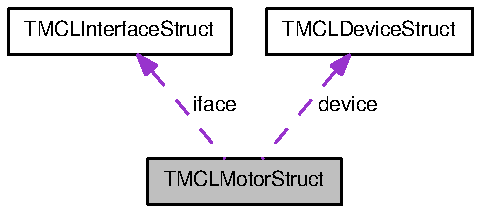
\includegraphics[width=266pt]{structTMCLMotorStruct__coll__graph}
\end{center}
\end{figure}
\subsection*{Data Fields}
\begin{DoxyCompactItemize}
\item 
\hypertarget{structTMCLMotorStruct_a035fa87a12ac1eb2cd585273080c3951}{
\hyperlink{structTMCLDeviceStruct}{TMCLDevice} {\bfseries device}}
\label{structTMCLMotorStruct_a035fa87a12ac1eb2cd585273080c3951}

\item 
\hypertarget{structTMCLMotorStruct_ae6d556412ee1450882d073678811e753}{
\hyperlink{structTMCLInterfaceStruct}{TMCLInterface} $\ast$ {\bfseries iface}}
\label{structTMCLMotorStruct_ae6d556412ee1450882d073678811e753}

\end{DoxyCompactItemize}


\subsection{Detailed Description}
Motor handler

Stores information about the motor and the interface of the controller board 

Definition at line 32 of file motor.h.

The documentation for this struct was generated from the following file:\begin{DoxyCompactItemize}
\item 
src/tmcl/\hyperlink{motor_8h}{motor.h}\end{DoxyCompactItemize}

\hypertarget{structTMCLReplyStruct}{
\section{TMCLReplyStruct Struct Reference}
\label{structTMCLReplyStruct}\index{TMCLReplyStruct@{TMCLReplyStruct}}
}


{\ttfamily \#include $<$src/tmcl/tmcldefs.h$>$}\subsection*{Data Fields}
\begin{DoxyCompactItemize}
\item 
uint8\_\-t \hyperlink{structTMCLReplyStruct_aa7bdb24d8ec498df4a2d2b067211a344}{reply\_\-address}
\item 
uint8\_\-t \hyperlink{structTMCLReplyStruct_ae3ebaa97b939afc79eb0efe8c6ba7e4f}{module\_\-address}
\item 
uint8\_\-t \hyperlink{structTMCLReplyStruct_a74072ff7b4d9d12df630545839131196}{status}
\item 
uint8\_\-t \hyperlink{structTMCLReplyStruct_a40395664fbaf18959cc62531d965a790}{command}
\item 
uint32\_\-t \hyperlink{structTMCLReplyStruct_aace5a128745c0f5b680a160b36cfaea6}{value}
\item 
uint8\_\-t \hyperlink{structTMCLReplyStruct_a64e2a7a1aedc90e4ba9200dcea006469}{checksum}
\end{DoxyCompactItemize}


\subsection{Detailed Description}
Structure for holding the reply of a module.

\begin{DoxySeeAlso}{See also}
\hyperlink{group__StatusCodes}{Status Codes.}, \hyperlink{group__TMCLComm}{TMCL commands.} 
\end{DoxySeeAlso}


Definition at line 283 of file tmcldefs.h.

\subsection{Field Documentation}
\hypertarget{structTMCLReplyStruct_a64e2a7a1aedc90e4ba9200dcea006469}{
\index{TMCLReplyStruct@{TMCLReplyStruct}!checksum@{checksum}}
\index{checksum@{checksum}!TMCLReplyStruct@{TMCLReplyStruct}}
\subsubsection[{checksum}]{\setlength{\rightskip}{0pt plus 5cm}uint8\_\-t {\bf TMCLReplyStruct::checksum}}}
\label{structTMCLReplyStruct_a64e2a7a1aedc90e4ba9200dcea006469}
Checksum 

Definition at line 289 of file tmcldefs.h.\hypertarget{structTMCLReplyStruct_a40395664fbaf18959cc62531d965a790}{
\index{TMCLReplyStruct@{TMCLReplyStruct}!command@{command}}
\index{command@{command}!TMCLReplyStruct@{TMCLReplyStruct}}
\subsubsection[{command}]{\setlength{\rightskip}{0pt plus 5cm}uint8\_\-t {\bf TMCLReplyStruct::command}}}
\label{structTMCLReplyStruct_a40395664fbaf18959cc62531d965a790}
Command 

Definition at line 287 of file tmcldefs.h.\hypertarget{structTMCLReplyStruct_ae3ebaa97b939afc79eb0efe8c6ba7e4f}{
\index{TMCLReplyStruct@{TMCLReplyStruct}!module\_\-address@{module\_\-address}}
\index{module\_\-address@{module\_\-address}!TMCLReplyStruct@{TMCLReplyStruct}}
\subsubsection[{module\_\-address}]{\setlength{\rightskip}{0pt plus 5cm}uint8\_\-t {\bf TMCLReplyStruct::module\_\-address}}}
\label{structTMCLReplyStruct_ae3ebaa97b939afc79eb0efe8c6ba7e4f}
Module address 

Definition at line 285 of file tmcldefs.h.\hypertarget{structTMCLReplyStruct_aa7bdb24d8ec498df4a2d2b067211a344}{
\index{TMCLReplyStruct@{TMCLReplyStruct}!reply\_\-address@{reply\_\-address}}
\index{reply\_\-address@{reply\_\-address}!TMCLReplyStruct@{TMCLReplyStruct}}
\subsubsection[{reply\_\-address}]{\setlength{\rightskip}{0pt plus 5cm}uint8\_\-t {\bf TMCLReplyStruct::reply\_\-address}}}
\label{structTMCLReplyStruct_aa7bdb24d8ec498df4a2d2b067211a344}
Reply address 

Definition at line 284 of file tmcldefs.h.\hypertarget{structTMCLReplyStruct_a74072ff7b4d9d12df630545839131196}{
\index{TMCLReplyStruct@{TMCLReplyStruct}!status@{status}}
\index{status@{status}!TMCLReplyStruct@{TMCLReplyStruct}}
\subsubsection[{status}]{\setlength{\rightskip}{0pt plus 5cm}uint8\_\-t {\bf TMCLReplyStruct::status}}}
\label{structTMCLReplyStruct_a74072ff7b4d9d12df630545839131196}
\hyperlink{group__StatusCodes}{Status Code} 

Definition at line 286 of file tmcldefs.h.\hypertarget{structTMCLReplyStruct_aace5a128745c0f5b680a160b36cfaea6}{
\index{TMCLReplyStruct@{TMCLReplyStruct}!value@{value}}
\index{value@{value}!TMCLReplyStruct@{TMCLReplyStruct}}
\subsubsection[{value}]{\setlength{\rightskip}{0pt plus 5cm}uint32\_\-t {\bf TMCLReplyStruct::value}}}
\label{structTMCLReplyStruct_aace5a128745c0f5b680a160b36cfaea6}
Value 

Definition at line 288 of file tmcldefs.h.

The documentation for this struct was generated from the following file:\begin{DoxyCompactItemize}
\item 
src/tmcl/\hyperlink{tmcldefs_8h}{tmcldefs.h}\end{DoxyCompactItemize}

\chapter{File Documentation}
\hypertarget{convenience_8h}{
\section{src/tmcl/convenience.h File Reference}
\label{convenience_8h}\index{src/tmcl/convenience.h@{src/tmcl/convenience.h}}
}
{\ttfamily \#include $<$inttypes.h$>$}\par
{\ttfamily \#include \char`\"{}motor.h\char`\"{}}\par
Include dependency graph for convenience.h:\nopagebreak
\begin{figure}[H]
\begin{center}
\leavevmode
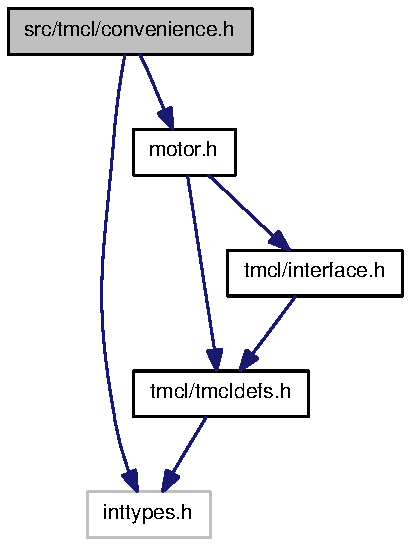
\includegraphics[width=116pt]{convenience_8h__incl}
\end{center}
\end{figure}
This graph shows which files directly or indirectly include this file:\nopagebreak
\begin{figure}[H]
\begin{center}
\leavevmode
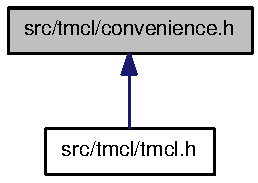
\includegraphics[width=80pt]{convenience_8h__dep__incl}
\end{center}
\end{figure}
\subsection*{Functions}
\begin{DoxyCompactItemize}
\item 
int \hyperlink{convenience_8h_ade9c1b3e4ada816b7bdd76d7fd2e1639}{tmcl\_\-move\_\-to\_\-pos\_\-abs} (\hyperlink{structTMCLMotorStruct}{TMCLMotor} $\ast$motor, int position)
\item 
int \hyperlink{convenience_8h_af1234e508a14ebfb3c2c6c0582fbb9d5}{tmcl\_\-move\_\-to\_\-pos\_\-rel} (\hyperlink{structTMCLMotorStruct}{TMCLMotor} $\ast$motor, int position)
\item 
int \hyperlink{convenience_8h_acde409988cd13a2928523516d1a203f9}{tmcl\_\-move\_\-to\_\-coord} (\hyperlink{structTMCLMotorStruct}{TMCLMotor} $\ast$motor, int coordinate)
\item 
int \hyperlink{convenience_8h_ac3dd7b3737010109df8b3bb800890bb7}{tmcl\_\-stop} (\hyperlink{structTMCLMotorStruct}{TMCLMotor} $\ast$motor)
\item 
int \hyperlink{convenience_8h_a002fe6b01caeb3a1c4c245e15d96d5f0}{tmcl\_\-refsearch\_\-start} (\hyperlink{structTMCLMotorStruct}{TMCLMotor} $\ast$motor)
\item 
int \hyperlink{convenience_8h_a5bbc946d3102331d43a010db44120149}{tmcl\_\-refsearch\_\-stop} (\hyperlink{structTMCLMotorStruct}{TMCLMotor} $\ast$motor)
\item 
int \hyperlink{convenience_8h_acd7a790f78576279e83008880905834e}{tmcl\_\-refsearch\_\-status} (\hyperlink{structTMCLMotorStruct}{TMCLMotor} $\ast$motor)
\item 
int32\_\-t \hyperlink{convenience_8h_a83b30f371b69aa1bb4062963128c8404}{tmcl\_\-get\_\-position} (\hyperlink{structTMCLMotorStruct}{TMCLMotor} $\ast$motor)
\item 
int \hyperlink{convenience_8h_a5f7be50971f8ee4a23abb0bfc796a3df}{tmcl\_\-ror} (\hyperlink{structTMCLMotorStruct}{TMCLMotor} $\ast$motor, int velocity)
\item 
int \hyperlink{convenience_8h_ab347aea7a694742e7f9968cb6663dc85}{tmcl\_\-rol} (\hyperlink{structTMCLMotorStruct}{TMCLMotor} $\ast$motor, int velocity)
\item 
int \hyperlink{convenience_8h_a28d15f70ff3338d6b36dd67bc30a0f3d}{tmcl\_\-set\_\-max\_\-current} (\hyperlink{structTMCLMotorStruct}{TMCLMotor} $\ast$motor, unsigned int percent)
\item 
int \hyperlink{convenience_8h_a52529417a99489b11f7bbd647fac8207}{tmcl\_\-get\_\-max\_\-current} (\hyperlink{structTMCLMotorStruct}{TMCLMotor} $\ast$motor)
\item 
int \hyperlink{convenience_8h_a1079e2a8e9a22a8279ace9befcf0c551}{tmcl\_\-set\_\-max\_\-standby\_\-current} (\hyperlink{structTMCLMotorStruct}{TMCLMotor} $\ast$motor, unsigned int percent)
\item 
int \hyperlink{convenience_8h_ae5c09e7de2fcd863cce97a4c34862ae1}{tmcl\_\-get\_\-max\_\-standby\_\-current} (\hyperlink{structTMCLMotorStruct}{TMCLMotor} $\ast$motor)
\item 
int \hyperlink{convenience_8h_a9b8738124f99ca6377b6b278e289d6a5}{tmcl\_\-set\_\-microsteps} (\hyperlink{structTMCLMotorStruct}{TMCLMotor} $\ast$motor, int microsteps)
\item 
int \hyperlink{convenience_8h_ab6498b8dabfb0bded2ff12488b86c4fe}{tmcl\_\-get\_\-microsteps} (\hyperlink{structTMCLMotorStruct}{TMCLMotor} $\ast$motor)
\item 
int \hyperlink{convenience_8h_abfa4f22d0004e1c6a6edae3720cbcd11}{tmcl\_\-activate\_\-limit\_\-switch} (\hyperlink{structTMCLMotorStruct}{TMCLMotor} $\ast$motor, int limit\_\-switch)
\item 
int \hyperlink{convenience_8h_aa64d4c054d237c284db2c76cde9c5070}{tmcl\_\-deactivate\_\-limit\_\-switch} (\hyperlink{structTMCLMotorStruct}{TMCLMotor} $\ast$motor, int limit\_\-switch)
\item 
int \hyperlink{convenience_8h_acb47891de6c40e7054f3ae15e85ab1f8}{tmcl\_\-get\_\-limit\_\-switch} (\hyperlink{structTMCLMotorStruct}{TMCLMotor} $\ast$motor, int limit\_\-switch)
\item 
int \hyperlink{convenience_8h_a2f5d78884d6cc87a6d31abf2932f4d81}{tmcl\_\-set\_\-no\_\-ref\_\-switch} (\hyperlink{structTMCLMotorStruct}{TMCLMotor} $\ast$motor, int number)
\item 
int \hyperlink{convenience_8h_a7c9af10e994fce71bb1055465176f16c}{tmcl\_\-get\_\-current\_\-speed} (\hyperlink{structTMCLMotorStruct}{TMCLMotor} $\ast$motor)
\item 
int \hyperlink{convenience_8h_abbdc689391aa6017a9accd1aa10eb958}{tmcl\_\-set\_\-refsearch\_\-speed} (\hyperlink{structTMCLMotorStruct}{TMCLMotor} $\ast$motor, int fraction)
\item 
int \hyperlink{convenience_8h_a8c63f30cf717dbed4e0efd63af435574}{tmcl\_\-get\_\-refsearch\_\-speed} (\hyperlink{structTMCLMotorStruct}{TMCLMotor} $\ast$motor)
\item 
int \hyperlink{convenience_8h_a56398eafa720e79aa9cbd73c309b2757}{tmcl\_\-set\_\-pos\_\-speed} (\hyperlink{structTMCLMotorStruct}{TMCLMotor} $\ast$motor, int speed)
\item 
int \hyperlink{convenience_8h_ae4eb2a19056c163bfe83e91db4847e19}{tmcl\_\-get\_\-pos\_\-speed} (\hyperlink{structTMCLMotorStruct}{TMCLMotor} $\ast$motor)
\item 
int \hyperlink{convenience_8h_a4099ac9f0bd1101fdd50dc5e97f86953}{tmcl\_\-get\_\-limit\_\-status} (\hyperlink{structTMCLMotorStruct}{TMCLMotor} $\ast$motor, int limit\_\-switch)
\end{DoxyCompactItemize}


\subsection{Detailed Description}
Convenience function for regularly used actions 

Definition in file \hyperlink{convenience_8h_source}{convenience.h}.

\subsection{Function Documentation}
\hypertarget{convenience_8h_abfa4f22d0004e1c6a6edae3720cbcd11}{
\index{convenience.h@{convenience.h}!tmcl\_\-activate\_\-limit\_\-switch@{tmcl\_\-activate\_\-limit\_\-switch}}
\index{tmcl\_\-activate\_\-limit\_\-switch@{tmcl\_\-activate\_\-limit\_\-switch}!convenience.h@{convenience.h}}
\subsubsection[{tmcl\_\-activate\_\-limit\_\-switch}]{\setlength{\rightskip}{0pt plus 5cm}int tmcl\_\-activate\_\-limit\_\-switch ({\bf TMCLMotor} $\ast$ {\em motor}, \/  int {\em limit\_\-switch})}}
\label{convenience_8h_abfa4f22d0004e1c6a6edae3720cbcd11}
Activate limit switch


\begin{DoxyParams}{Parameters}
\item[\mbox{$\leftarrow$} {\em limit\_\-switch}]ID of limit switch to activate\end{DoxyParams}
\begin{DoxyReturn}{Returns}

\begin{DoxyItemize}
\item 0 on success
\item -\/1 on failure 
\end{DoxyItemize}
\end{DoxyReturn}


Definition at line 410 of file convenience.c.\hypertarget{convenience_8h_aa64d4c054d237c284db2c76cde9c5070}{
\index{convenience.h@{convenience.h}!tmcl\_\-deactivate\_\-limit\_\-switch@{tmcl\_\-deactivate\_\-limit\_\-switch}}
\index{tmcl\_\-deactivate\_\-limit\_\-switch@{tmcl\_\-deactivate\_\-limit\_\-switch}!convenience.h@{convenience.h}}
\subsubsection[{tmcl\_\-deactivate\_\-limit\_\-switch}]{\setlength{\rightskip}{0pt plus 5cm}int tmcl\_\-deactivate\_\-limit\_\-switch ({\bf TMCLMotor} $\ast$ {\em motor}, \/  int {\em limit\_\-switch})}}
\label{convenience_8h_aa64d4c054d237c284db2c76cde9c5070}
Deactivate limit switch


\begin{DoxyParams}{Parameters}
\item[\mbox{$\leftarrow$} {\em limit\_\-switch}]ID of limit switch to deactivate\end{DoxyParams}
\begin{DoxyReturn}{Returns}

\begin{DoxyItemize}
\item 0 on success
\item -\/1 on failure 
\end{DoxyItemize}
\end{DoxyReturn}


Definition at line 415 of file convenience.c.\hypertarget{convenience_8h_a7c9af10e994fce71bb1055465176f16c}{
\index{convenience.h@{convenience.h}!tmcl\_\-get\_\-current\_\-speed@{tmcl\_\-get\_\-current\_\-speed}}
\index{tmcl\_\-get\_\-current\_\-speed@{tmcl\_\-get\_\-current\_\-speed}!convenience.h@{convenience.h}}
\subsubsection[{tmcl\_\-get\_\-current\_\-speed}]{\setlength{\rightskip}{0pt plus 5cm}int tmcl\_\-get\_\-current\_\-speed ({\bf TMCLMotor} $\ast$ {\em motor})}}
\label{convenience_8h_a7c9af10e994fce71bb1055465176f16c}
Get current speed of motor

\begin{DoxyReturn}{Returns}

\begin{DoxyItemize}
\item $>$=0: current speed of motor
\item -\/1 on failure 
\end{DoxyItemize}
\end{DoxyReturn}


Definition at line 482 of file convenience.c.\hypertarget{convenience_8h_a4099ac9f0bd1101fdd50dc5e97f86953}{
\index{convenience.h@{convenience.h}!tmcl\_\-get\_\-limit\_\-status@{tmcl\_\-get\_\-limit\_\-status}}
\index{tmcl\_\-get\_\-limit\_\-status@{tmcl\_\-get\_\-limit\_\-status}!convenience.h@{convenience.h}}
\subsubsection[{tmcl\_\-get\_\-limit\_\-status}]{\setlength{\rightskip}{0pt plus 5cm}int tmcl\_\-get\_\-limit\_\-status ({\bf TMCLMotor} $\ast$ {\em motor}, \/  int {\em limit\_\-switch})}}
\label{convenience_8h_a4099ac9f0bd1101fdd50dc5e97f86953}
Get status of limit switch


\begin{DoxyParams}{Parameters}
\item[\mbox{$\leftarrow$} {\em limit\_\-switch}]Limit switch to check 0: left switch, 1: right switch\end{DoxyParams}
\begin{DoxyReturn}{Returns}

\begin{DoxyItemize}
\item 0: when limit switch is open
\item 1: when limit switch is closed
\item -\/1: on failure 
\end{DoxyItemize}
\end{DoxyReturn}


Definition at line 504 of file convenience.c.\hypertarget{convenience_8h_acb47891de6c40e7054f3ae15e85ab1f8}{
\index{convenience.h@{convenience.h}!tmcl\_\-get\_\-limit\_\-switch@{tmcl\_\-get\_\-limit\_\-switch}}
\index{tmcl\_\-get\_\-limit\_\-switch@{tmcl\_\-get\_\-limit\_\-switch}!convenience.h@{convenience.h}}
\subsubsection[{tmcl\_\-get\_\-limit\_\-switch}]{\setlength{\rightskip}{0pt plus 5cm}int tmcl\_\-get\_\-limit\_\-switch ({\bf TMCLMotor} $\ast$ {\em motor}, \/  int {\em limit\_\-switch})}}
\label{convenience_8h_acb47891de6c40e7054f3ae15e85ab1f8}
Check if limit switch is active


\begin{DoxyParams}{Parameters}
\item[\mbox{$\leftarrow$} {\em limit\_\-switch}]Switch to check\end{DoxyParams}
\begin{DoxyReturn}{Returns}

\begin{DoxyItemize}
\item 1 when {\ttfamily limit\_\-switch} is active
\item 0 when not active
\item -\/1 on error 
\end{DoxyItemize}
\end{DoxyReturn}


Definition at line 384 of file convenience.c.\hypertarget{convenience_8h_a52529417a99489b11f7bbd647fac8207}{
\index{convenience.h@{convenience.h}!tmcl\_\-get\_\-max\_\-current@{tmcl\_\-get\_\-max\_\-current}}
\index{tmcl\_\-get\_\-max\_\-current@{tmcl\_\-get\_\-max\_\-current}!convenience.h@{convenience.h}}
\subsubsection[{tmcl\_\-get\_\-max\_\-current}]{\setlength{\rightskip}{0pt plus 5cm}int tmcl\_\-get\_\-max\_\-current ({\bf TMCLMotor} $\ast$ {\em motor})}}
\label{convenience_8h_a52529417a99489b11f7bbd647fac8207}
Get maximum current

\begin{DoxyReturn}{Returns}

\begin{DoxyItemize}
\item current in percent of available full current
\item -\/1 on error 
\end{DoxyItemize}
\end{DoxyReturn}


Definition at line 248 of file convenience.c.\hypertarget{convenience_8h_ae5c09e7de2fcd863cce97a4c34862ae1}{
\index{convenience.h@{convenience.h}!tmcl\_\-get\_\-max\_\-standby\_\-current@{tmcl\_\-get\_\-max\_\-standby\_\-current}}
\index{tmcl\_\-get\_\-max\_\-standby\_\-current@{tmcl\_\-get\_\-max\_\-standby\_\-current}!convenience.h@{convenience.h}}
\subsubsection[{tmcl\_\-get\_\-max\_\-standby\_\-current}]{\setlength{\rightskip}{0pt plus 5cm}int tmcl\_\-get\_\-max\_\-standby\_\-current ({\bf TMCLMotor} $\ast$ {\em motor})}}
\label{convenience_8h_ae5c09e7de2fcd863cce97a4c34862ae1}
Get maximum standby current

\begin{DoxyReturn}{Returns}

\begin{DoxyItemize}
\item current in percent of available full current
\item -\/1 on error 
\end{DoxyItemize}
\end{DoxyReturn}


Definition at line 272 of file convenience.c.\hypertarget{convenience_8h_ab6498b8dabfb0bded2ff12488b86c4fe}{
\index{convenience.h@{convenience.h}!tmcl\_\-get\_\-microsteps@{tmcl\_\-get\_\-microsteps}}
\index{tmcl\_\-get\_\-microsteps@{tmcl\_\-get\_\-microsteps}!convenience.h@{convenience.h}}
\subsubsection[{tmcl\_\-get\_\-microsteps}]{\setlength{\rightskip}{0pt plus 5cm}int tmcl\_\-get\_\-microsteps ({\bf TMCLMotor} $\ast$ {\em motor})}}
\label{convenience_8h_ab6498b8dabfb0bded2ff12488b86c4fe}
Get used microsteps

\begin{DoxyNote}{Note}
not for TMCM100 model
\end{DoxyNote}
\begin{DoxyReturn}{Returns}

\begin{DoxyItemize}
\item microsteps: 0 (full step mode), 1 (half step mode), 2, 4, 8, 16, 32, 64 microsteps
\item -\/1 on failure 
\end{DoxyItemize}
\end{DoxyReturn}


Definition at line 320 of file convenience.c.\hypertarget{convenience_8h_ae4eb2a19056c163bfe83e91db4847e19}{
\index{convenience.h@{convenience.h}!tmcl\_\-get\_\-pos\_\-speed@{tmcl\_\-get\_\-pos\_\-speed}}
\index{tmcl\_\-get\_\-pos\_\-speed@{tmcl\_\-get\_\-pos\_\-speed}!convenience.h@{convenience.h}}
\subsubsection[{tmcl\_\-get\_\-pos\_\-speed}]{\setlength{\rightskip}{0pt plus 5cm}int tmcl\_\-get\_\-pos\_\-speed ({\bf TMCLMotor} $\ast$ {\em motor})}}
\label{convenience_8h_ae4eb2a19056c163bfe83e91db4847e19}
Get positioning speed 

Definition at line 498 of file convenience.c.\hypertarget{convenience_8h_a83b30f371b69aa1bb4062963128c8404}{
\index{convenience.h@{convenience.h}!tmcl\_\-get\_\-position@{tmcl\_\-get\_\-position}}
\index{tmcl\_\-get\_\-position@{tmcl\_\-get\_\-position}!convenience.h@{convenience.h}}
\subsubsection[{tmcl\_\-get\_\-position}]{\setlength{\rightskip}{0pt plus 5cm}int32\_\-t tmcl\_\-get\_\-position ({\bf TMCLMotor} $\ast$ {\em motor})}}
\label{convenience_8h_a83b30f371b69aa1bb4062963128c8404}
Get current position of motor 

Definition at line 166 of file convenience.c.\hypertarget{convenience_8h_a8c63f30cf717dbed4e0efd63af435574}{
\index{convenience.h@{convenience.h}!tmcl\_\-get\_\-refsearch\_\-speed@{tmcl\_\-get\_\-refsearch\_\-speed}}
\index{tmcl\_\-get\_\-refsearch\_\-speed@{tmcl\_\-get\_\-refsearch\_\-speed}!convenience.h@{convenience.h}}
\subsubsection[{tmcl\_\-get\_\-refsearch\_\-speed}]{\setlength{\rightskip}{0pt plus 5cm}int tmcl\_\-get\_\-refsearch\_\-speed ({\bf TMCLMotor} $\ast$ {\em motor})}}
\label{convenience_8h_a8c63f30cf717dbed4e0efd63af435574}
Get reference search speed

\begin{DoxyReturn}{Returns}

\begin{DoxyItemize}
\item $>$=0: reference search speed in fraction of positioning speed
\item -\/1: failure 
\end{DoxyItemize}
\end{DoxyReturn}


Definition at line 477 of file convenience.c.\hypertarget{convenience_8h_acde409988cd13a2928523516d1a203f9}{
\index{convenience.h@{convenience.h}!tmcl\_\-move\_\-to\_\-coord@{tmcl\_\-move\_\-to\_\-coord}}
\index{tmcl\_\-move\_\-to\_\-coord@{tmcl\_\-move\_\-to\_\-coord}!convenience.h@{convenience.h}}
\subsubsection[{tmcl\_\-move\_\-to\_\-coord}]{\setlength{\rightskip}{0pt plus 5cm}int tmcl\_\-move\_\-to\_\-coord ({\bf TMCLMotor} $\ast$ {\em motor}, \/  int {\em coordinate})}}
\label{convenience_8h_acde409988cd13a2928523516d1a203f9}
Move to previously stored coordinate See TMCL reference for details 

Definition at line 76 of file convenience.c.\hypertarget{convenience_8h_ade9c1b3e4ada816b7bdd76d7fd2e1639}{
\index{convenience.h@{convenience.h}!tmcl\_\-move\_\-to\_\-pos\_\-abs@{tmcl\_\-move\_\-to\_\-pos\_\-abs}}
\index{tmcl\_\-move\_\-to\_\-pos\_\-abs@{tmcl\_\-move\_\-to\_\-pos\_\-abs}!convenience.h@{convenience.h}}
\subsubsection[{tmcl\_\-move\_\-to\_\-pos\_\-abs}]{\setlength{\rightskip}{0pt plus 5cm}int tmcl\_\-move\_\-to\_\-pos\_\-abs ({\bf TMCLMotor} $\ast$ {\em motor}, \/  int {\em position})}}
\label{convenience_8h_ade9c1b3e4ada816b7bdd76d7fd2e1639}
Move motor to absolute position 

Definition at line 26 of file convenience.c.\hypertarget{convenience_8h_af1234e508a14ebfb3c2c6c0582fbb9d5}{
\index{convenience.h@{convenience.h}!tmcl\_\-move\_\-to\_\-pos\_\-rel@{tmcl\_\-move\_\-to\_\-pos\_\-rel}}
\index{tmcl\_\-move\_\-to\_\-pos\_\-rel@{tmcl\_\-move\_\-to\_\-pos\_\-rel}!convenience.h@{convenience.h}}
\subsubsection[{tmcl\_\-move\_\-to\_\-pos\_\-rel}]{\setlength{\rightskip}{0pt plus 5cm}int tmcl\_\-move\_\-to\_\-pos\_\-rel ({\bf TMCLMotor} $\ast$ {\em motor}, \/  int {\em position})}}
\label{convenience_8h_af1234e508a14ebfb3c2c6c0582fbb9d5}
Move motor relative to current position 

Definition at line 63 of file convenience.c.\hypertarget{convenience_8h_a002fe6b01caeb3a1c4c245e15d96d5f0}{
\index{convenience.h@{convenience.h}!tmcl\_\-refsearch\_\-start@{tmcl\_\-refsearch\_\-start}}
\index{tmcl\_\-refsearch\_\-start@{tmcl\_\-refsearch\_\-start}!convenience.h@{convenience.h}}
\subsubsection[{tmcl\_\-refsearch\_\-start}]{\setlength{\rightskip}{0pt plus 5cm}int tmcl\_\-refsearch\_\-start ({\bf TMCLMotor} $\ast$ {\em motor})}}
\label{convenience_8h_a002fe6b01caeb3a1c4c245e15d96d5f0}
Start reference search 

Definition at line 101 of file convenience.c.\hypertarget{convenience_8h_acd7a790f78576279e83008880905834e}{
\index{convenience.h@{convenience.h}!tmcl\_\-refsearch\_\-status@{tmcl\_\-refsearch\_\-status}}
\index{tmcl\_\-refsearch\_\-status@{tmcl\_\-refsearch\_\-status}!convenience.h@{convenience.h}}
\subsubsection[{tmcl\_\-refsearch\_\-status}]{\setlength{\rightskip}{0pt plus 5cm}int tmcl\_\-refsearch\_\-status ({\bf TMCLMotor} $\ast$ {\em motor})}}
\label{convenience_8h_acd7a790f78576279e83008880905834e}
Get status of reference search

\begin{DoxyReturn}{Returns}

\begin{DoxyItemize}
\item 1 when reference search is running
\item 0 when no reference search is running
\item -\/1 on error 
\end{DoxyItemize}
\end{DoxyReturn}


Definition at line 137 of file convenience.c.\hypertarget{convenience_8h_a5bbc946d3102331d43a010db44120149}{
\index{convenience.h@{convenience.h}!tmcl\_\-refsearch\_\-stop@{tmcl\_\-refsearch\_\-stop}}
\index{tmcl\_\-refsearch\_\-stop@{tmcl\_\-refsearch\_\-stop}!convenience.h@{convenience.h}}
\subsubsection[{tmcl\_\-refsearch\_\-stop}]{\setlength{\rightskip}{0pt plus 5cm}int tmcl\_\-refsearch\_\-stop ({\bf TMCLMotor} $\ast$ {\em motor})}}
\label{convenience_8h_a5bbc946d3102331d43a010db44120149}
Stop reference search 

Definition at line 118 of file convenience.c.\hypertarget{convenience_8h_ab347aea7a694742e7f9968cb6663dc85}{
\index{convenience.h@{convenience.h}!tmcl\_\-rol@{tmcl\_\-rol}}
\index{tmcl\_\-rol@{tmcl\_\-rol}!convenience.h@{convenience.h}}
\subsubsection[{tmcl\_\-rol}]{\setlength{\rightskip}{0pt plus 5cm}int tmcl\_\-rol ({\bf TMCLMotor} $\ast$ {\em motor}, \/  int {\em velocity})}}
\label{convenience_8h_ab347aea7a694742e7f9968cb6663dc85}
Rotate motor left 

Definition at line 51 of file convenience.c.\hypertarget{convenience_8h_a5f7be50971f8ee4a23abb0bfc796a3df}{
\index{convenience.h@{convenience.h}!tmcl\_\-ror@{tmcl\_\-ror}}
\index{tmcl\_\-ror@{tmcl\_\-ror}!convenience.h@{convenience.h}}
\subsubsection[{tmcl\_\-ror}]{\setlength{\rightskip}{0pt plus 5cm}int tmcl\_\-ror ({\bf TMCLMotor} $\ast$ {\em motor}, \/  int {\em velocity})}}
\label{convenience_8h_a5f7be50971f8ee4a23abb0bfc796a3df}
Rotate motor right 

Definition at line 39 of file convenience.c.\hypertarget{convenience_8h_a28d15f70ff3338d6b36dd67bc30a0f3d}{
\index{convenience.h@{convenience.h}!tmcl\_\-set\_\-max\_\-current@{tmcl\_\-set\_\-max\_\-current}}
\index{tmcl\_\-set\_\-max\_\-current@{tmcl\_\-set\_\-max\_\-current}!convenience.h@{convenience.h}}
\subsubsection[{tmcl\_\-set\_\-max\_\-current}]{\setlength{\rightskip}{0pt plus 5cm}int tmcl\_\-set\_\-max\_\-current ({\bf TMCLMotor} $\ast$ {\em motor}, \/  unsigned int {\em percent})}}
\label{convenience_8h_a28d15f70ff3338d6b36dd67bc30a0f3d}
Set maximum current


\begin{DoxyParams}{Parameters}
\item[\mbox{$\leftarrow$} {\em current}]in percent of full current \end{DoxyParams}


Definition at line 231 of file convenience.c.\hypertarget{convenience_8h_a1079e2a8e9a22a8279ace9befcf0c551}{
\index{convenience.h@{convenience.h}!tmcl\_\-set\_\-max\_\-standby\_\-current@{tmcl\_\-set\_\-max\_\-standby\_\-current}}
\index{tmcl\_\-set\_\-max\_\-standby\_\-current@{tmcl\_\-set\_\-max\_\-standby\_\-current}!convenience.h@{convenience.h}}
\subsubsection[{tmcl\_\-set\_\-max\_\-standby\_\-current}]{\setlength{\rightskip}{0pt plus 5cm}int tmcl\_\-set\_\-max\_\-standby\_\-current ({\bf TMCLMotor} $\ast$ {\em motor}, \/  unsigned int {\em percent})}}
\label{convenience_8h_a1079e2a8e9a22a8279ace9befcf0c551}
Set maximum standby current


\begin{DoxyParams}{Parameters}
\item[\mbox{$\leftarrow$} {\em maximum}]standby current in percent \end{DoxyParams}


Definition at line 257 of file convenience.c.\hypertarget{convenience_8h_a9b8738124f99ca6377b6b278e289d6a5}{
\index{convenience.h@{convenience.h}!tmcl\_\-set\_\-microsteps@{tmcl\_\-set\_\-microsteps}}
\index{tmcl\_\-set\_\-microsteps@{tmcl\_\-set\_\-microsteps}!convenience.h@{convenience.h}}
\subsubsection[{tmcl\_\-set\_\-microsteps}]{\setlength{\rightskip}{0pt plus 5cm}int tmcl\_\-set\_\-microsteps ({\bf TMCLMotor} $\ast$ {\em motor}, \/  int {\em microsteps})}}
\label{convenience_8h_a9b8738124f99ca6377b6b278e289d6a5}
Set microsteps for movement

\begin{DoxyNote}{Note}
not for TMCM100 model
\end{DoxyNote}

\begin{DoxyParams}{Parameters}
\item[\mbox{$\leftarrow$} {\em microsteps}]0 (full step mode), 1 (half step mode), 2, 4, 8, 16, 32, 64 microsteps \end{DoxyParams}


Definition at line 281 of file convenience.c.\hypertarget{convenience_8h_a2f5d78884d6cc87a6d31abf2932f4d81}{
\index{convenience.h@{convenience.h}!tmcl\_\-set\_\-no\_\-ref\_\-switch@{tmcl\_\-set\_\-no\_\-ref\_\-switch}}
\index{tmcl\_\-set\_\-no\_\-ref\_\-switch@{tmcl\_\-set\_\-no\_\-ref\_\-switch}!convenience.h@{convenience.h}}
\subsubsection[{tmcl\_\-set\_\-no\_\-ref\_\-switch}]{\setlength{\rightskip}{0pt plus 5cm}int tmcl\_\-set\_\-no\_\-ref\_\-switch ({\bf TMCLMotor} $\ast$ {\em motor}, \/  int {\em number})}}
\label{convenience_8h_a2f5d78884d6cc87a6d31abf2932f4d81}
Set number of reference switches


\begin{DoxyParams}{Parameters}
\item[\mbox{$\leftarrow$} {\em number}]Number of reference switches (1-\/3)\end{DoxyParams}
\begin{DoxyReturn}{Returns}

\begin{DoxyItemize}
\item 0 on success
\item -\/1 on failure 
\end{DoxyItemize}
\end{DoxyReturn}


Definition at line 420 of file convenience.c.\hypertarget{convenience_8h_a56398eafa720e79aa9cbd73c309b2757}{
\index{convenience.h@{convenience.h}!tmcl\_\-set\_\-pos\_\-speed@{tmcl\_\-set\_\-pos\_\-speed}}
\index{tmcl\_\-set\_\-pos\_\-speed@{tmcl\_\-set\_\-pos\_\-speed}!convenience.h@{convenience.h}}
\subsubsection[{tmcl\_\-set\_\-pos\_\-speed}]{\setlength{\rightskip}{0pt plus 5cm}int tmcl\_\-set\_\-pos\_\-speed ({\bf TMCLMotor} $\ast$ {\em motor}, \/  int {\em speed})}}
\label{convenience_8h_a56398eafa720e79aa9cbd73c309b2757}
Set positioning speed


\begin{DoxyParams}{Parameters}
\item[\mbox{$\leftarrow$} {\em speed}]Positioning speed 0-\/2047\end{DoxyParams}
\begin{DoxyReturn}{Returns}

\begin{DoxyItemize}
\item 0 on success
\item -\/1 on failure 
\end{DoxyItemize}
\end{DoxyReturn}


Definition at line 488 of file convenience.c.\hypertarget{convenience_8h_abbdc689391aa6017a9accd1aa10eb958}{
\index{convenience.h@{convenience.h}!tmcl\_\-set\_\-refsearch\_\-speed@{tmcl\_\-set\_\-refsearch\_\-speed}}
\index{tmcl\_\-set\_\-refsearch\_\-speed@{tmcl\_\-set\_\-refsearch\_\-speed}!convenience.h@{convenience.h}}
\subsubsection[{tmcl\_\-set\_\-refsearch\_\-speed}]{\setlength{\rightskip}{0pt plus 5cm}int tmcl\_\-set\_\-refsearch\_\-speed ({\bf TMCLMotor} $\ast$ {\em motor}, \/  int {\em fraction})}}
\label{convenience_8h_abbdc689391aa6017a9accd1aa10eb958}
Set reference search speed


\begin{DoxyParams}{Parameters}
\item[\mbox{$\leftarrow$} {\em fraction}]Set reference search speed to 1/fraction of positioning speed \end{DoxyParams}


Definition at line 453 of file convenience.c.\hypertarget{convenience_8h_ac3dd7b3737010109df8b3bb800890bb7}{
\index{convenience.h@{convenience.h}!tmcl\_\-stop@{tmcl\_\-stop}}
\index{tmcl\_\-stop@{tmcl\_\-stop}!convenience.h@{convenience.h}}
\subsubsection[{tmcl\_\-stop}]{\setlength{\rightskip}{0pt plus 5cm}int tmcl\_\-stop ({\bf TMCLMotor} $\ast$ {\em motor})}}
\label{convenience_8h_ac3dd7b3737010109df8b3bb800890bb7}
Stop motor 

Definition at line 89 of file convenience.c.
\hypertarget{interface_8h}{
\section{src/tmcl/interface.h File Reference}
\label{interface_8h}\index{src/tmcl/interface.h@{src/tmcl/interface.h}}
}
{\ttfamily \#include $<$tmcl/tmcldefs.h$>$}\par
Include dependency graph for interface.h:\nopagebreak
\begin{figure}[H]
\begin{center}
\leavevmode
\includegraphics[width=72pt]{interface_8h__incl}
\end{center}
\end{figure}
This graph shows which files directly or indirectly include this file:\nopagebreak
\begin{figure}[H]
\begin{center}
\leavevmode
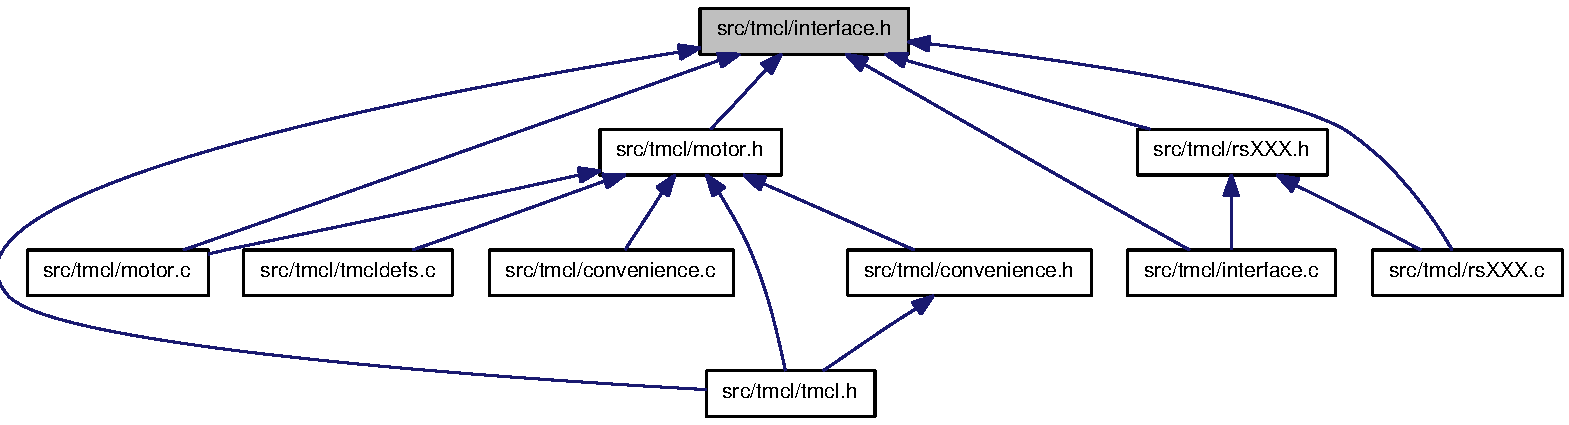
\includegraphics[width=394pt]{interface_8h__dep__incl}
\end{center}
\end{figure}
\subsection*{Data Structures}
\begin{DoxyCompactItemize}
\item 
struct \hyperlink{structTMCLInterfaceStruct}{TMCLInterfaceStruct}
\end{DoxyCompactItemize}
\subsection*{Typedefs}
\begin{DoxyCompactItemize}
\item 
typedef int($\ast$ \hyperlink{interface_8h_a1f8f6db177582534470f015805447f32}{tmcl\_\-open\_\-funcPtr} )(struct \hyperlink{structTMCLInterfaceStruct}{TMCLInterfaceStruct} $\ast$iface, const char $\ast$ifacename, void $\ast$)
\item 
\hypertarget{interface_8h_a9e7227a8c5d13beb62425dc812ffa50d}{
typedef int($\ast$ {\bfseries tmcl\_\-close\_\-funcPtr} )(struct \hyperlink{structTMCLInterfaceStruct}{TMCLInterfaceStruct} $\ast$iface, void $\ast$)}
\label{interface_8h_a9e7227a8c5d13beb62425dc812ffa50d}

\item 
\hypertarget{interface_8h_a4e986ad65eb977300f1a85a10667877a}{
typedef int($\ast$ {\bfseries tmcl\_\-write\_\-funcPtr} )(struct \hyperlink{structTMCLInterfaceStruct}{TMCLInterfaceStruct} $\ast$iface, const void $\ast$buffer, int length, void $\ast$)}
\label{interface_8h_a4e986ad65eb977300f1a85a10667877a}

\item 
\hypertarget{interface_8h_a1f18ca4d75f24fb75ae4415f025cc7f7}{
typedef int($\ast$ {\bfseries tmcl\_\-read\_\-funcPtr} )(struct \hyperlink{structTMCLInterfaceStruct}{TMCLInterfaceStruct} $\ast$iface, char $\ast$buffer, void $\ast$)}
\label{interface_8h_a1f18ca4d75f24fb75ae4415f025cc7f7}

\item 
typedef struct \hyperlink{structTMCLInterfaceStruct}{TMCLInterfaceStruct} \hyperlink{interface_8h_a02607838b81b4bec6053a0781186c20d}{TMCLInterface}
\end{DoxyCompactItemize}
\subsection*{Functions}
\begin{DoxyCompactItemize}
\item 
int \hyperlink{interface_8h_a6234d4f85bda5c0132fdecde69565ef4}{tmcl\_\-init\_\-interface} (\hyperlink{structTMCLInterfaceStruct}{TMCLInterface} $\ast$$\ast$iface, \hyperlink{tmcldefs_8h_ad26e4e286a55d7c739fd473d8cdd882e}{TMCLBusType} bus, \hyperlink{interface_8h_a1f8f6db177582534470f015805447f32}{tmcl\_\-open\_\-funcPtr} open, tmcl\_\-close\_\-funcPtr close, tmcl\_\-read\_\-funcPtr read, tmcl\_\-write\_\-funcPtr write)
\item 
void \hyperlink{interface_8h_a4cf02ca59d140317d11d965e6ae95e26}{tmcl\_\-set\_\-open\_\-data} (\hyperlink{structTMCLInterfaceStruct}{TMCLInterface} $\ast$iface, void $\ast$func\_\-pointer)
\item 
void \hyperlink{interface_8h_a928addfc26628720283c4710165e279e}{tmcl\_\-set\_\-close\_\-data} (\hyperlink{structTMCLInterfaceStruct}{TMCLInterface} $\ast$iface, void $\ast$func\_\-pointer)
\item 
void \hyperlink{interface_8h_a2ab1e5dc50c5cf71d9e3524b0854f077}{tmcl\_\-set\_\-read\_\-data} (\hyperlink{structTMCLInterfaceStruct}{TMCLInterface} $\ast$iface, void $\ast$func\_\-pointer)
\item 
void \hyperlink{interface_8h_a971ed663d2191ec0503be6e098de4d33}{tmcl\_\-set\_\-write\_\-data} (\hyperlink{structTMCLInterfaceStruct}{TMCLInterface} $\ast$iface, void $\ast$func\_\-pointer)
\item 
void \hyperlink{interface_8h_a382b00c7bcc1c135272e7d4d14e493b8}{tmcl\_\-deinit\_\-interface} (\hyperlink{structTMCLInterfaceStruct}{TMCLInterface} $\ast$$\ast$iface)
\item 
int \hyperlink{interface_8h_a319f1f4969ffd9faebe4fef0c49d31bb}{tmcl\_\-open\_\-interface} (\hyperlink{structTMCLInterfaceStruct}{TMCLInterface} $\ast$iface, const char $\ast$filename)
\item 
int \hyperlink{interface_8h_ab78b0151f64fbbeae0567e8db9d39487}{tmcl\_\-close\_\-interface} (\hyperlink{structTMCLInterfaceStruct}{TMCLInterface} $\ast$iface)
\item 
void \hyperlink{interface_8h_a8e317645c487f3c5c1ef8365c2e1733d}{tmcl\_\-interface\_\-set\_\-timeout} (\hyperlink{structTMCLInterfaceStruct}{TMCLInterface} $\ast$iface, unsigned int sec, unsigned int msec)
\item 
void \hyperlink{interface_8h_af99259a37abb7f9d89847dcec8321254}{tmcl\_\-interface\_\-set\_\-timewait} (\hyperlink{structTMCLInterfaceStruct}{TMCLInterface} $\ast$iface, unsigned int sec, unsigned int msec)
\end{DoxyCompactItemize}


\subsection{Detailed Description}
Functions, structures, etc. to access the interface of the controller board 

Definition in file \hyperlink{interface_8h_source}{interface.h}.

\subsection{Typedef Documentation}
\hypertarget{interface_8h_a1f8f6db177582534470f015805447f32}{
\index{interface.h@{interface.h}!tmcl\_\-open\_\-funcPtr@{tmcl\_\-open\_\-funcPtr}}
\index{tmcl\_\-open\_\-funcPtr@{tmcl\_\-open\_\-funcPtr}!interface.h@{interface.h}}
\subsubsection[{tmcl\_\-open\_\-funcPtr}]{\setlength{\rightskip}{0pt plus 5cm}typedef int($\ast$ {\bf tmcl\_\-open\_\-funcPtr})(struct {\bf TMCLInterfaceStruct} $\ast$iface, const char $\ast$ifacename, void $\ast$)}}
\label{interface_8h_a1f8f6db177582534470f015805447f32}
Function pointers for open/close and read/write interface communication functions 

Definition at line 30 of file interface.h.\hypertarget{interface_8h_a02607838b81b4bec6053a0781186c20d}{
\index{interface.h@{interface.h}!TMCLInterface@{TMCLInterface}}
\index{TMCLInterface@{TMCLInterface}!interface.h@{interface.h}}
\subsubsection[{TMCLInterface}]{\setlength{\rightskip}{0pt plus 5cm}typedef struct {\bf TMCLInterfaceStruct}  {\bf TMCLInterface}}}
\label{interface_8h_a02607838b81b4bec6053a0781186c20d}
Struct to store information about the controller interface 

\subsection{Function Documentation}
\hypertarget{interface_8h_ab78b0151f64fbbeae0567e8db9d39487}{
\index{interface.h@{interface.h}!tmcl\_\-close\_\-interface@{tmcl\_\-close\_\-interface}}
\index{tmcl\_\-close\_\-interface@{tmcl\_\-close\_\-interface}!interface.h@{interface.h}}
\subsubsection[{tmcl\_\-close\_\-interface}]{\setlength{\rightskip}{0pt plus 5cm}int tmcl\_\-close\_\-interface ({\bf TMCLInterface} $\ast$ {\em iface})}}
\label{interface_8h_ab78b0151f64fbbeae0567e8db9d39487}
Close interface $\ast$

\begin{DoxyReturn}{Returns}

\begin{DoxyItemize}
\item 0 on success
\item -\/1 on failure 
\end{DoxyItemize}
\end{DoxyReturn}


Definition at line 130 of file interface.c.\hypertarget{interface_8h_a382b00c7bcc1c135272e7d4d14e493b8}{
\index{interface.h@{interface.h}!tmcl\_\-deinit\_\-interface@{tmcl\_\-deinit\_\-interface}}
\index{tmcl\_\-deinit\_\-interface@{tmcl\_\-deinit\_\-interface}!interface.h@{interface.h}}
\subsubsection[{tmcl\_\-deinit\_\-interface}]{\setlength{\rightskip}{0pt plus 5cm}void tmcl\_\-deinit\_\-interface ({\bf TMCLInterface} $\ast$$\ast$ {\em iface})}}
\label{interface_8h_a382b00c7bcc1c135272e7d4d14e493b8}
Deinitialize interface 

Definition at line 107 of file interface.c.\hypertarget{interface_8h_a6234d4f85bda5c0132fdecde69565ef4}{
\index{interface.h@{interface.h}!tmcl\_\-init\_\-interface@{tmcl\_\-init\_\-interface}}
\index{tmcl\_\-init\_\-interface@{tmcl\_\-init\_\-interface}!interface.h@{interface.h}}
\subsubsection[{tmcl\_\-init\_\-interface}]{\setlength{\rightskip}{0pt plus 5cm}int tmcl\_\-init\_\-interface ({\bf TMCLInterface} $\ast$$\ast$ {\em iface}, \/  {\bf TMCLBusType} {\em bus}, \/  {\bf tmcl\_\-open\_\-funcPtr} {\em open}, \/  tmcl\_\-close\_\-funcPtr {\em close}, \/  tmcl\_\-read\_\-funcPtr {\em read}, \/  tmcl\_\-write\_\-funcPtr {\em write})}}
\label{interface_8h_a6234d4f85bda5c0132fdecde69565ef4}
Initialize TMCLInterface struct

Custom open/close/read/write functions may be given here. Use {\ttfamily NULL} to use the builtin functions.

\begin{DoxyReturn}{Returns}

\begin{DoxyItemize}
\item 0 on success
\item -\/1 on failure 
\end{DoxyItemize}
\end{DoxyReturn}


Definition at line 39 of file interface.c.\hypertarget{interface_8h_a8e317645c487f3c5c1ef8365c2e1733d}{
\index{interface.h@{interface.h}!tmcl\_\-interface\_\-set\_\-timeout@{tmcl\_\-interface\_\-set\_\-timeout}}
\index{tmcl\_\-interface\_\-set\_\-timeout@{tmcl\_\-interface\_\-set\_\-timeout}!interface.h@{interface.h}}
\subsubsection[{tmcl\_\-interface\_\-set\_\-timeout}]{\setlength{\rightskip}{0pt plus 5cm}void tmcl\_\-interface\_\-set\_\-timeout ({\bf TMCLInterface} $\ast$ {\em iface}, \/  unsigned int {\em sec}, \/  unsigned int {\em msec})}}
\label{interface_8h_a8e317645c487f3c5c1ef8365c2e1733d}
Adjust timout for interface communication 

Definition at line 143 of file interface.c.\hypertarget{interface_8h_af99259a37abb7f9d89847dcec8321254}{
\index{interface.h@{interface.h}!tmcl\_\-interface\_\-set\_\-timewait@{tmcl\_\-interface\_\-set\_\-timewait}}
\index{tmcl\_\-interface\_\-set\_\-timewait@{tmcl\_\-interface\_\-set\_\-timewait}!interface.h@{interface.h}}
\subsubsection[{tmcl\_\-interface\_\-set\_\-timewait}]{\setlength{\rightskip}{0pt plus 5cm}void tmcl\_\-interface\_\-set\_\-timewait ({\bf TMCLInterface} $\ast$ {\em iface}, \/  unsigned int {\em sec}, \/  unsigned int {\em msec})}}
\label{interface_8h_af99259a37abb7f9d89847dcec8321254}
Adjust how long to wait for reply from motor controller 

Definition at line 151 of file interface.c.\hypertarget{interface_8h_a319f1f4969ffd9faebe4fef0c49d31bb}{
\index{interface.h@{interface.h}!tmcl\_\-open\_\-interface@{tmcl\_\-open\_\-interface}}
\index{tmcl\_\-open\_\-interface@{tmcl\_\-open\_\-interface}!interface.h@{interface.h}}
\subsubsection[{tmcl\_\-open\_\-interface}]{\setlength{\rightskip}{0pt plus 5cm}int tmcl\_\-open\_\-interface ({\bf TMCLInterface} $\ast$ {\em iface}, \/  const char $\ast$ {\em filename})}}
\label{interface_8h_a319f1f4969ffd9faebe4fef0c49d31bb}
Open interface $\ast$


\begin{DoxyParams}{Parameters}
\item[\mbox{$\leftarrow$} {\em iface}]TMCLInterface struct \item[\mbox{$\leftarrow$} {\em filename}]filename of interface device (for RSXXX)\end{DoxyParams}
\begin{DoxyReturn}{Returns}

\begin{DoxyItemize}
\item 0 on success
\item -\/1 on failure 
\end{DoxyItemize}
\end{DoxyReturn}


Definition at line 113 of file interface.c.\hypertarget{interface_8h_a928addfc26628720283c4710165e279e}{
\index{interface.h@{interface.h}!tmcl\_\-set\_\-close\_\-data@{tmcl\_\-set\_\-close\_\-data}}
\index{tmcl\_\-set\_\-close\_\-data@{tmcl\_\-set\_\-close\_\-data}!interface.h@{interface.h}}
\subsubsection[{tmcl\_\-set\_\-close\_\-data}]{\setlength{\rightskip}{0pt plus 5cm}void tmcl\_\-set\_\-close\_\-data ({\bf TMCLInterface} $\ast$ {\em iface}, \/  void $\ast$ {\em func\_\-pointer})}}
\label{interface_8h_a928addfc26628720283c4710165e279e}
Set custom close function for interface 

Definition at line 95 of file interface.c.\hypertarget{interface_8h_a4cf02ca59d140317d11d965e6ae95e26}{
\index{interface.h@{interface.h}!tmcl\_\-set\_\-open\_\-data@{tmcl\_\-set\_\-open\_\-data}}
\index{tmcl\_\-set\_\-open\_\-data@{tmcl\_\-set\_\-open\_\-data}!interface.h@{interface.h}}
\subsubsection[{tmcl\_\-set\_\-open\_\-data}]{\setlength{\rightskip}{0pt plus 5cm}void tmcl\_\-set\_\-open\_\-data ({\bf TMCLInterface} $\ast$ {\em iface}, \/  void $\ast$ {\em func\_\-pointer})}}
\label{interface_8h_a4cf02ca59d140317d11d965e6ae95e26}
Set custom open function for interface 

Definition at line 91 of file interface.c.\hypertarget{interface_8h_a2ab1e5dc50c5cf71d9e3524b0854f077}{
\index{interface.h@{interface.h}!tmcl\_\-set\_\-read\_\-data@{tmcl\_\-set\_\-read\_\-data}}
\index{tmcl\_\-set\_\-read\_\-data@{tmcl\_\-set\_\-read\_\-data}!interface.h@{interface.h}}
\subsubsection[{tmcl\_\-set\_\-read\_\-data}]{\setlength{\rightskip}{0pt plus 5cm}void tmcl\_\-set\_\-read\_\-data ({\bf TMCLInterface} $\ast$ {\em iface}, \/  void $\ast$ {\em func\_\-pointer})}}
\label{interface_8h_a2ab1e5dc50c5cf71d9e3524b0854f077}
Set custom read function for interface 

Definition at line 99 of file interface.c.\hypertarget{interface_8h_a971ed663d2191ec0503be6e098de4d33}{
\index{interface.h@{interface.h}!tmcl\_\-set\_\-write\_\-data@{tmcl\_\-set\_\-write\_\-data}}
\index{tmcl\_\-set\_\-write\_\-data@{tmcl\_\-set\_\-write\_\-data}!interface.h@{interface.h}}
\subsubsection[{tmcl\_\-set\_\-write\_\-data}]{\setlength{\rightskip}{0pt plus 5cm}void tmcl\_\-set\_\-write\_\-data ({\bf TMCLInterface} $\ast$ {\em iface}, \/  void $\ast$ {\em func\_\-pointer})}}
\label{interface_8h_a971ed663d2191ec0503be6e098de4d33}
Set custom write function for interface 

Definition at line 103 of file interface.c.
\hypertarget{motor_8h}{
\section{src/tmcl/motor.h File Reference}
\label{motor_8h}\index{src/tmcl/motor.h@{src/tmcl/motor.h}}
}
{\ttfamily \#include $<$tmcl/tmcldefs.h$>$}\par
{\ttfamily \#include $<$tmcl/interface.h$>$}\par
Include dependency graph for motor.h:\nopagebreak
\begin{figure}[H]
\begin{center}
\leavevmode
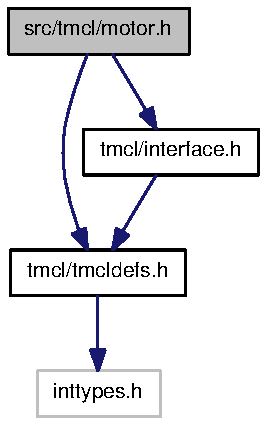
\includegraphics[width=82pt]{motor_8h__incl}
\end{center}
\end{figure}
This graph shows which files directly or indirectly include this file:\nopagebreak
\begin{figure}[H]
\begin{center}
\leavevmode
\includegraphics[width=277pt]{motor_8h__dep__incl}
\end{center}
\end{figure}
\subsection*{Data Structures}
\begin{DoxyCompactItemize}
\item 
struct \hyperlink{structTMCLMotorStruct}{TMCLMotorStruct}
\end{DoxyCompactItemize}
\subsection*{Typedefs}
\begin{DoxyCompactItemize}
\item 
typedef struct \hyperlink{structTMCLMotorStruct}{TMCLMotorStruct} \hyperlink{motor_8h_a14d786be976dfa481c05b4b712eca059}{TMCLMotor}
\end{DoxyCompactItemize}
\subsection*{Functions}
\begin{DoxyCompactItemize}
\item 
int \hyperlink{motor_8h_a54fa9817766cc27bca3f7542ab748cc2}{tmcl\_\-init\_\-motor} (\hyperlink{structTMCLMotorStruct}{TMCLMotor} $\ast$$\ast$mot, \hyperlink{structTMCLInterfaceStruct}{TMCLInterface} $\ast$iface, \hyperlink{tmcldefs_8h_a35c090090de43d9850d0f573f7d29e45}{TMCLModel} model, uint8\_\-t address, uint8\_\-t bank, \hyperlink{tmcldefs_8h_ad26e4e286a55d7c739fd473d8cdd882e}{TMCLBusType} bus)
\item 
void \hyperlink{motor_8h_a925e764d84777a9dc131546dd1b32699}{tmcl\_\-deinit\_\-motor} (\hyperlink{structTMCLMotorStruct}{TMCLMotor} $\ast$$\ast$mot)
\item 
int \hyperlink{motor_8h_a0994799e6eeee41f70093c081bdc7d0a}{tmcl\_\-send\_\-command} (\hyperlink{structTMCLMotorStruct}{TMCLMotor} $\ast$mot, \hyperlink{structTMCLCommandStruct}{TMCLCommand} tcom, \hyperlink{structTMCLReplyStruct}{TMCLReply} $\ast$reply)
\item 
int \hyperlink{motor_8h_ac2cbc887882b38608ea63deb10f684bc}{tmcl\_\-update\_\-axis\_\-parameter} (\hyperlink{structTMCLMotorStruct}{TMCLMotor} $\ast$mot, int axis\_\-parameter)
\item 
int \hyperlink{motor_8h_a55a0a1ad09c44b1386a528b4e74f3962}{tmcl\_\-set\_\-axis\_\-parameter} (\hyperlink{structTMCLMotorStruct}{TMCLMotor} $\ast$mot, int axis\_\-parameter, int value)
\item 
int \hyperlink{motor_8h_acde6e9e540c95467c08ad479ca3627cd}{tmcl\_\-get\_\-axis\_\-parameter} (\hyperlink{structTMCLMotorStruct}{TMCLMotor} $\ast$mot, int axis\_\-parameter)
\item 
int \hyperlink{motor_8h_a943cbb77b0d0bf244742c34211d03c17}{tmcl\_\-store\_\-axis\_\-parameter} (\hyperlink{structTMCLMotorStruct}{TMCLMotor} $\ast$mot, int axis\_\-parameter)
\end{DoxyCompactItemize}


\subsection{Detailed Description}
Motor communication and configuration 

Definition in file \hyperlink{motor_8h_source}{motor.h}.

\subsection{Typedef Documentation}
\hypertarget{motor_8h_a14d786be976dfa481c05b4b712eca059}{
\index{motor.h@{motor.h}!TMCLMotor@{TMCLMotor}}
\index{TMCLMotor@{TMCLMotor}!motor.h@{motor.h}}
\subsubsection[{TMCLMotor}]{\setlength{\rightskip}{0pt plus 5cm}typedef struct {\bf TMCLMotorStruct}
 {\bf TMCLMotor}}}
\label{motor_8h_a14d786be976dfa481c05b4b712eca059}
Motor handler

Stores information about the motor and the interface of the controller board 

\subsection{Function Documentation}
\hypertarget{motor_8h_a925e764d84777a9dc131546dd1b32699}{
\index{motor.h@{motor.h}!tmcl\_\-deinit\_\-motor@{tmcl\_\-deinit\_\-motor}}
\index{tmcl\_\-deinit\_\-motor@{tmcl\_\-deinit\_\-motor}!motor.h@{motor.h}}
\subsubsection[{tmcl\_\-deinit\_\-motor}]{\setlength{\rightskip}{0pt plus 5cm}void tmcl\_\-deinit\_\-motor ({\bf TMCLMotor} $\ast$$\ast$ {\em mot})}}
\label{motor_8h_a925e764d84777a9dc131546dd1b32699}
Deinitialize motor handling structure 

Definition at line 57 of file motor.c.\hypertarget{motor_8h_acde6e9e540c95467c08ad479ca3627cd}{
\index{motor.h@{motor.h}!tmcl\_\-get\_\-axis\_\-parameter@{tmcl\_\-get\_\-axis\_\-parameter}}
\index{tmcl\_\-get\_\-axis\_\-parameter@{tmcl\_\-get\_\-axis\_\-parameter}!motor.h@{motor.h}}
\subsubsection[{tmcl\_\-get\_\-axis\_\-parameter}]{\setlength{\rightskip}{0pt plus 5cm}int tmcl\_\-get\_\-axis\_\-parameter ({\bf TMCLMotor} $\ast$ {\em mot}, \/  int {\em axis\_\-parameter})}}
\label{motor_8h_acde6e9e540c95467c08ad479ca3627cd}
Get axis parameter from motor struct

This does not read the parameter from the board, but just from the TMCLMotor struct. To update the value in the TMCLMotor struct call \hyperlink{motor_8h_ac2cbc887882b38608ea63deb10f684bc}{tmcl\_\-update\_\-axis\_\-parameter()} before.


\begin{DoxyParams}{Parameters}
\item[\mbox{$\leftarrow$} {\em mot}]Motor struct \item[\mbox{$\leftarrow$} {\em axis\_\-parameter}]Parameter to get \end{DoxyParams}
\begin{DoxySeeAlso}{See also}
\hyperlink{group__AxisParam}{Axis Parameters}
\end{DoxySeeAlso}
\begin{DoxyReturn}{Returns}

\begin{DoxyItemize}
\item 0: on success
\item -\/1: on failure 
\end{DoxyItemize}
\end{DoxyReturn}


Definition at line 173 of file motor.c.\hypertarget{motor_8h_a54fa9817766cc27bca3f7542ab748cc2}{
\index{motor.h@{motor.h}!tmcl\_\-init\_\-motor@{tmcl\_\-init\_\-motor}}
\index{tmcl\_\-init\_\-motor@{tmcl\_\-init\_\-motor}!motor.h@{motor.h}}
\subsubsection[{tmcl\_\-init\_\-motor}]{\setlength{\rightskip}{0pt plus 5cm}int tmcl\_\-init\_\-motor ({\bf TMCLMotor} $\ast$$\ast$ {\em mot}, \/  {\bf TMCLInterface} $\ast$ {\em iface}, \/  {\bf TMCLModel} {\em model}, \/  uint8\_\-t {\em address}, \/  uint8\_\-t {\em bank}, \/  {\bf TMCLBusType} {\em bus})}}
\label{motor_8h_a54fa9817766cc27bca3f7542ab748cc2}
Initialize motor handling structure

\begin{DoxyReturn}{Returns}

\begin{DoxyItemize}
\item 0: on success
\item -\/1: on failure 
\end{DoxyItemize}
\end{DoxyReturn}


Definition at line 30 of file motor.c.\hypertarget{motor_8h_a0994799e6eeee41f70093c081bdc7d0a}{
\index{motor.h@{motor.h}!tmcl\_\-send\_\-command@{tmcl\_\-send\_\-command}}
\index{tmcl\_\-send\_\-command@{tmcl\_\-send\_\-command}!motor.h@{motor.h}}
\subsubsection[{tmcl\_\-send\_\-command}]{\setlength{\rightskip}{0pt plus 5cm}int tmcl\_\-send\_\-command ({\bf TMCLMotor} $\ast$ {\em mot}, \/  {\bf TMCLCommand} {\em tcom}, \/  {\bf TMCLReply} $\ast$ {\em reply})}}
\label{motor_8h_a0994799e6eeee41f70093c081bdc7d0a}
Send command to motor

\begin{DoxySeeAlso}{See also}
\hyperlink{tmcldefs_8h_a61ff3e5938eeb8d7a5b41fcba8f7c914}{TMCLCommand}
\end{DoxySeeAlso}
\begin{DoxyReturn}{Returns}

\begin{DoxyItemize}
\item 0: on success
\item -\/1: on failure 
\end{DoxyItemize}
\end{DoxyReturn}


Definition at line 69 of file motor.c.\hypertarget{motor_8h_a55a0a1ad09c44b1386a528b4e74f3962}{
\index{motor.h@{motor.h}!tmcl\_\-set\_\-axis\_\-parameter@{tmcl\_\-set\_\-axis\_\-parameter}}
\index{tmcl\_\-set\_\-axis\_\-parameter@{tmcl\_\-set\_\-axis\_\-parameter}!motor.h@{motor.h}}
\subsubsection[{tmcl\_\-set\_\-axis\_\-parameter}]{\setlength{\rightskip}{0pt plus 5cm}int tmcl\_\-set\_\-axis\_\-parameter ({\bf TMCLMotor} $\ast$ {\em mot}, \/  int {\em axis\_\-parameter}, \/  int {\em value})}}
\label{motor_8h_a55a0a1ad09c44b1386a528b4e74f3962}
Set axis parameter in motor controller board


\begin{DoxyParams}{Parameters}
\item[\mbox{$\leftarrow$} {\em mot}]Motor struct \item[\mbox{$\leftarrow$} {\em axis\_\-parameter}]Parameter to set \end{DoxyParams}
\begin{DoxySeeAlso}{See also}
\hyperlink{group__AxisParam}{Axis Parameters} 
\end{DoxySeeAlso}

\begin{DoxyParams}{Parameters}
\item[\mbox{$\leftarrow$} {\em value}]New value for parameter\end{DoxyParams}
\begin{DoxyReturn}{Returns}

\begin{DoxyItemize}
\item 0: on success
\item -\/1: on failure 
\end{DoxyItemize}
\end{DoxyReturn}


Definition at line 184 of file motor.c.\hypertarget{motor_8h_a943cbb77b0d0bf244742c34211d03c17}{
\index{motor.h@{motor.h}!tmcl\_\-store\_\-axis\_\-parameter@{tmcl\_\-store\_\-axis\_\-parameter}}
\index{tmcl\_\-store\_\-axis\_\-parameter@{tmcl\_\-store\_\-axis\_\-parameter}!motor.h@{motor.h}}
\subsubsection[{tmcl\_\-store\_\-axis\_\-parameter}]{\setlength{\rightskip}{0pt plus 5cm}int tmcl\_\-store\_\-axis\_\-parameter ({\bf TMCLMotor} $\ast$ {\em mot}, \/  int {\em axis\_\-parameter})}}
\label{motor_8h_a943cbb77b0d0bf244742c34211d03c17}
Read all available axis parameters from the controller board and store them in the TMCLMotor struct

\begin{DoxyReturn}{Returns}

\begin{DoxyItemize}
\item 0: on success
\item -\/1: on failure
\end{DoxyItemize}
\end{DoxyReturn}
\begin{Desc}
\item[\hyperlink{todo__todo000001}{Todo}]: Currently broken and thus not commented \end{Desc}
Copy axis parameter from RAM to non-\/volatile EEPROM on board

\begin{DoxyReturn}{Returns}

\begin{DoxyItemize}
\item 0: on success
\item -\/1: on failure 
\end{DoxyItemize}
\end{DoxyReturn}


Definition at line 213 of file motor.c.\hypertarget{motor_8h_ac2cbc887882b38608ea63deb10f684bc}{
\index{motor.h@{motor.h}!tmcl\_\-update\_\-axis\_\-parameter@{tmcl\_\-update\_\-axis\_\-parameter}}
\index{tmcl\_\-update\_\-axis\_\-parameter@{tmcl\_\-update\_\-axis\_\-parameter}!motor.h@{motor.h}}
\subsubsection[{tmcl\_\-update\_\-axis\_\-parameter}]{\setlength{\rightskip}{0pt plus 5cm}int tmcl\_\-update\_\-axis\_\-parameter ({\bf TMCLMotor} $\ast$ {\em mot}, \/  int {\em axis\_\-parameter})}}
\label{motor_8h_ac2cbc887882b38608ea63deb10f684bc}
Read axis parameter 'axis\_\-parameter' from the motor and saves it in the 'TMCLMotor' struct


\begin{DoxyParams}{Parameters}
\item[\mbox{$\leftarrow$} {\em mot}]Motor struct \item[\mbox{$\leftarrow$} {\em tmcl\_\-parameter}]Parameter to read\end{DoxyParams}
\begin{DoxyReturn}{Returns}

\begin{DoxyItemize}
\item 0: on success
\item -\/1: on failure 
\end{DoxyItemize}
\end{DoxyReturn}


Definition at line 141 of file motor.c.
\hypertarget{rsXXX_8h}{
\section{src/tmcl/rsXXX.h File Reference}
\label{rsXXX_8h}\index{src/tmcl/rsXXX.h@{src/tmcl/rsXXX.h}}
}
{\ttfamily \#include $<$tmcl/tmcldefs.h$>$}\par
{\ttfamily \#include $<$tmcl/interface.h$>$}\par
Include dependency graph for rsXXX.h:\nopagebreak
\begin{figure}[H]
\begin{center}
\leavevmode
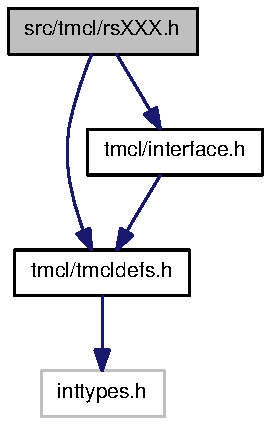
\includegraphics[width=83pt]{rsXXX_8h__incl}
\end{center}
\end{figure}
This graph shows which files directly or indirectly include this file:\nopagebreak
\begin{figure}[H]
\begin{center}
\leavevmode
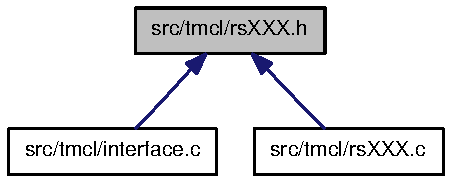
\includegraphics[width=126pt]{rsXXX_8h__dep__incl}
\end{center}
\end{figure}
\subsection*{Functions}
\begin{DoxyCompactItemize}
\item 
int \hyperlink{rsXXX_8h_a3d01e21594c18d248fa6a7ad769c0769}{tmcl\_\-open\_\-rsXXX} (\hyperlink{structTMCLInterfaceStruct}{TMCLInterface} $\ast$iface, const char $\ast$filename, void $\ast$pointer)
\item 
int \hyperlink{rsXXX_8h_a0ac132ac213a306a829db1f98ea6517b}{tmcl\_\-close\_\-rsXXX} (\hyperlink{structTMCLInterfaceStruct}{TMCLInterface} $\ast$iface, void $\ast$pointer)
\item 
int \hyperlink{rsXXX_8h_a29d4db3ce6b3756743a51d3b1ccb49d1}{tmcl\_\-write\_\-rsXXX} (\hyperlink{structTMCLInterfaceStruct}{TMCLInterface} $\ast$iface, const void $\ast$buf, int length, void $\ast$pointer)
\item 
int \hyperlink{rsXXX_8h_aa8017d8e9d05727a7d6958865061c087}{tmcl\_\-poll\_\-rsXXX} (\hyperlink{structTMCLInterfaceStruct}{TMCLInterface} $\ast$iface, char $\ast$buffer, void $\ast$pointer)
\end{DoxyCompactItemize}


\subsection{Detailed Description}
Communication function for RS232 and RS485 interfaces

Normally there should not be any need to call these directly. 

Definition in file \hyperlink{rsXXX_8h_source}{rsXXX.h}.

\subsection{Function Documentation}
\hypertarget{rsXXX_8h_a0ac132ac213a306a829db1f98ea6517b}{
\index{rsXXX.h@{rsXXX.h}!tmcl\_\-close\_\-rsXXX@{tmcl\_\-close\_\-rsXXX}}
\index{tmcl\_\-close\_\-rsXXX@{tmcl\_\-close\_\-rsXXX}!rsXXX.h@{rsXXX.h}}
\subsubsection[{tmcl\_\-close\_\-rsXXX}]{\setlength{\rightskip}{0pt plus 5cm}int tmcl\_\-close\_\-rsXXX ({\bf TMCLInterface} $\ast$ {\em iface}, \/  void $\ast$ {\em pointer})}}
\label{rsXXX_8h_a0ac132ac213a306a829db1f98ea6517b}
Closes the RSXXX port

\begin{DoxyItemize}
\item {\ttfamily pointer:} NOT USED!\end{DoxyItemize}
Returns:
\begin{DoxyItemize}
\item 0 on success
\item -\/1 on failure 
\end{DoxyItemize}

Definition at line 143 of file rsXXX.c.\hypertarget{rsXXX_8h_a3d01e21594c18d248fa6a7ad769c0769}{
\index{rsXXX.h@{rsXXX.h}!tmcl\_\-open\_\-rsXXX@{tmcl\_\-open\_\-rsXXX}}
\index{tmcl\_\-open\_\-rsXXX@{tmcl\_\-open\_\-rsXXX}!rsXXX.h@{rsXXX.h}}
\subsubsection[{tmcl\_\-open\_\-rsXXX}]{\setlength{\rightskip}{0pt plus 5cm}int tmcl\_\-open\_\-rsXXX ({\bf TMCLInterface} $\ast$ {\em iface}, \/  const char $\ast$ {\em filename}, \/  void $\ast$ {\em pointer})}}
\label{rsXXX_8h_a3d01e21594c18d248fa6a7ad769c0769}
Opens the RSXXX port

\begin{DoxyItemize}
\item {\ttfamily filename:} Device node of RSXXX port \item {\ttfamily pointer:} NOT USED!\end{DoxyItemize}
Returns:
\begin{DoxyItemize}
\item File descriptor of RSXXX port on success
\item -\/1 on failure 
\end{DoxyItemize}

Definition at line 128 of file rsXXX.c.\hypertarget{rsXXX_8h_aa8017d8e9d05727a7d6958865061c087}{
\index{rsXXX.h@{rsXXX.h}!tmcl\_\-poll\_\-rsXXX@{tmcl\_\-poll\_\-rsXXX}}
\index{tmcl\_\-poll\_\-rsXXX@{tmcl\_\-poll\_\-rsXXX}!rsXXX.h@{rsXXX.h}}
\subsubsection[{tmcl\_\-poll\_\-rsXXX}]{\setlength{\rightskip}{0pt plus 5cm}int tmcl\_\-poll\_\-rsXXX ({\bf TMCLInterface} $\ast$ {\em iface}, \/  char $\ast$ {\em buffer}, \/  void $\ast$ {\em pointer})}}
\label{rsXXX_8h_aa8017d8e9d05727a7d6958865061c087}
Waits for data from the RSXXX port.

\begin{DoxyItemize}
\item {\ttfamily buffer:} Buffer to store received data \item {\ttfamily pointer:} NOT USED! RETURNS
\begin{DoxyItemize}
\item $>$0: length of data read (in bytes)
\item -\/1 on failure
\item -\/2 on wrong length of read data 
\end{DoxyItemize}\end{DoxyItemize}


Definition at line 170 of file rsXXX.c.\hypertarget{rsXXX_8h_a29d4db3ce6b3756743a51d3b1ccb49d1}{
\index{rsXXX.h@{rsXXX.h}!tmcl\_\-write\_\-rsXXX@{tmcl\_\-write\_\-rsXXX}}
\index{tmcl\_\-write\_\-rsXXX@{tmcl\_\-write\_\-rsXXX}!rsXXX.h@{rsXXX.h}}
\subsubsection[{tmcl\_\-write\_\-rsXXX}]{\setlength{\rightskip}{0pt plus 5cm}int tmcl\_\-write\_\-rsXXX ({\bf TMCLInterface} $\ast$ {\em iface}, \/  const void $\ast$ {\em buf}, \/  int {\em length}, \/  void $\ast$ {\em pointer})}}
\label{rsXXX_8h_a29d4db3ce6b3756743a51d3b1ccb49d1}
Writes to RSXXX port

\begin{DoxyItemize}
\item {\ttfamily buf:} buffer of data to be written \item {\ttfamily length:} length of data buffer \item {\ttfamily pointer:} NOT USED!\end{DoxyItemize}
Returns:
\begin{DoxyItemize}
\item 0 on success
\item -\/1 on failure 
\end{DoxyItemize}

Definition at line 154 of file rsXXX.c.
\hypertarget{tmcl_8h}{
\section{src/tmcl/tmcl.h File Reference}
\label{tmcl_8h}\index{src/tmcl/tmcl.h@{src/tmcl/tmcl.h}}
}
{\ttfamily \#include $<$tmcl/tmcldefs.h$>$}\par
{\ttfamily \#include $<$tmcl/motor.h$>$}\par
{\ttfamily \#include $<$tmcl/convenience.h$>$}\par
{\ttfamily \#include $<$tmcl/interface.h$>$}\par
Include dependency graph for tmcl.h:\nopagebreak
\begin{figure}[H]
\begin{center}
\leavevmode
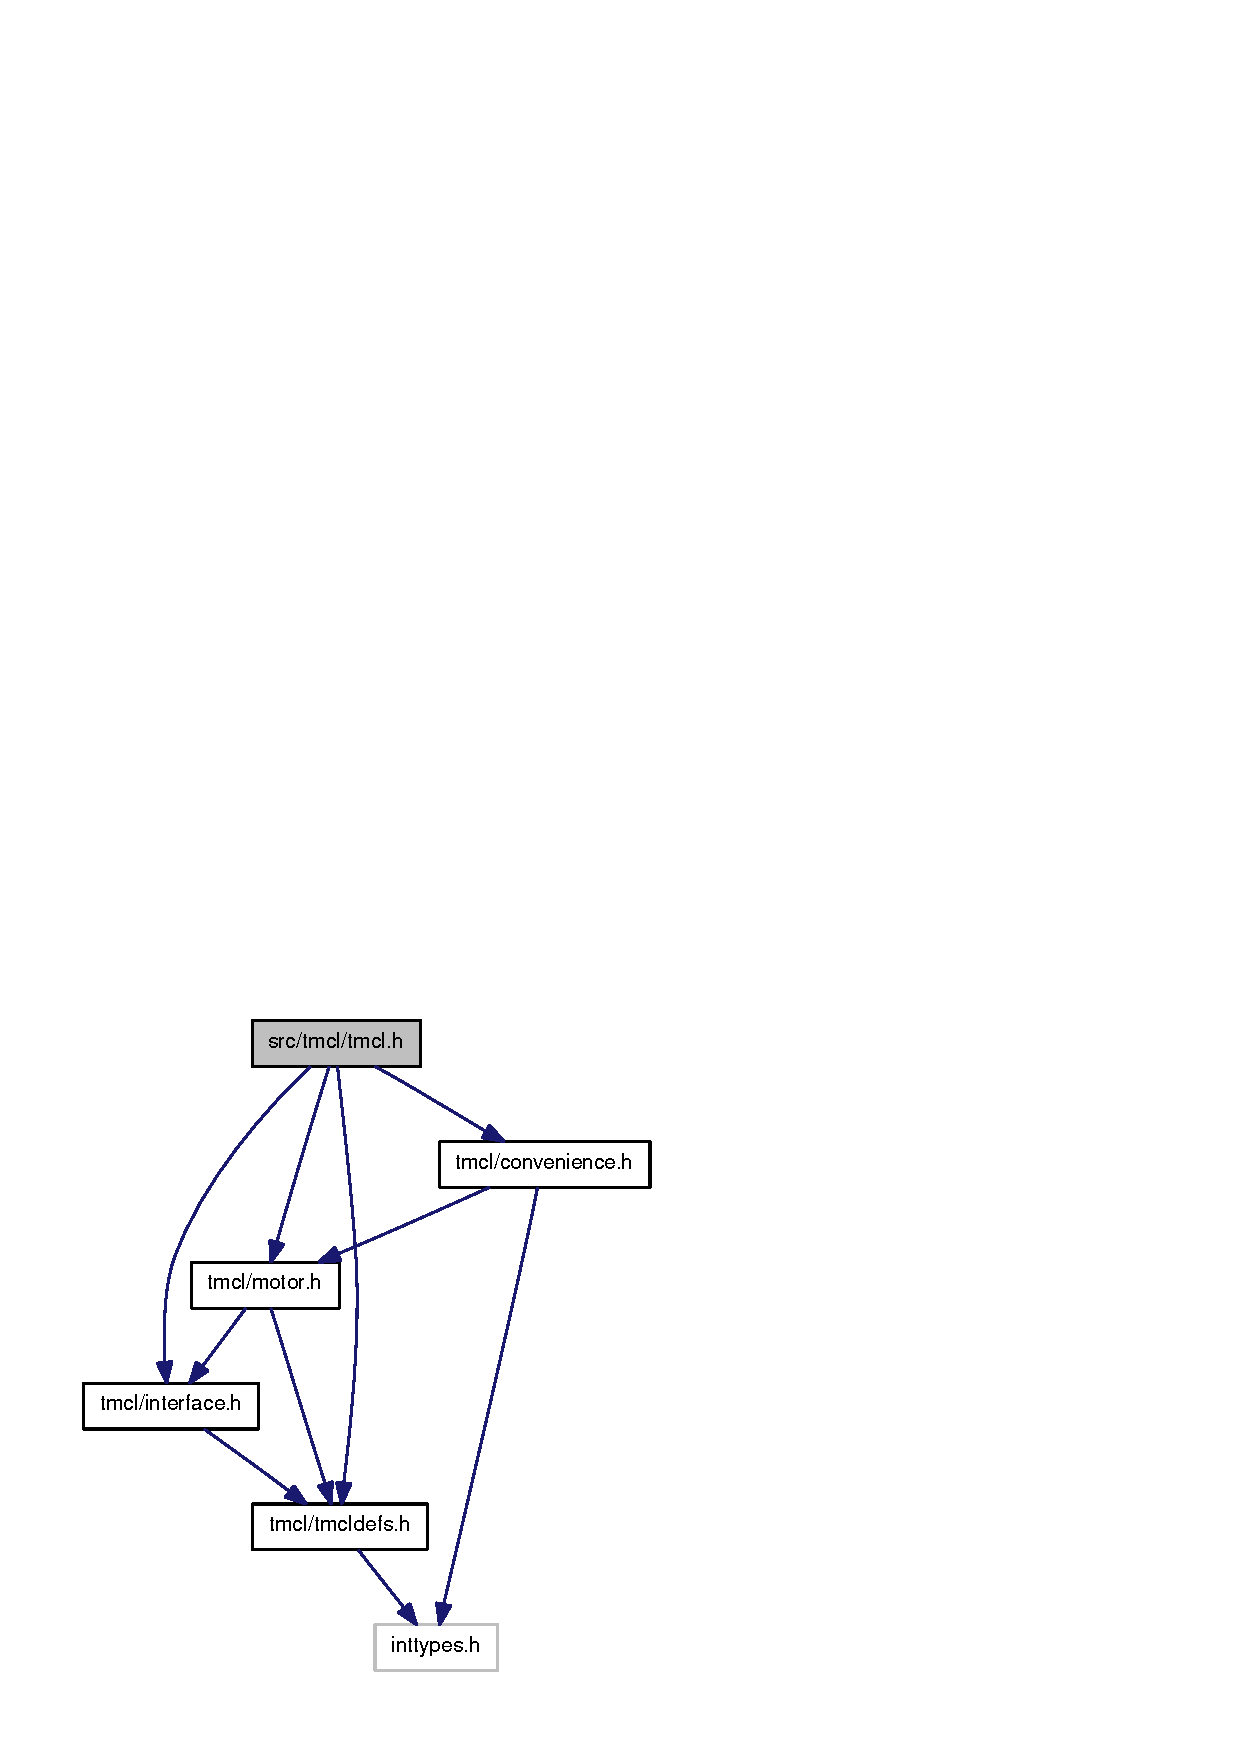
\includegraphics[width=157pt]{tmcl_8h__incl}
\end{center}
\end{figure}


\subsection{Detailed Description}
Main libtmcl include 

Definition in file \hyperlink{tmcl_8h_source}{tmcl.h}.
\hypertarget{tmcldefs_8c}{
\section{src/tmcl/tmcldefs.c File Reference}
\label{tmcldefs_8c}\index{src/tmcl/tmcldefs.c@{src/tmcl/tmcldefs.c}}
}
{\ttfamily \#include $<$assert.h$>$}\par
{\ttfamily \#include \char`\"{}tmcldefs.h\char`\"{}}\par
{\ttfamily \#include \char`\"{}motor.h\char`\"{}}\par
{\ttfamily \#include \char`\"{}debug.h\char`\"{}}\par
Include dependency graph for tmcldefs.c:\nopagebreak
\begin{figure}[H]
\begin{center}
\leavevmode
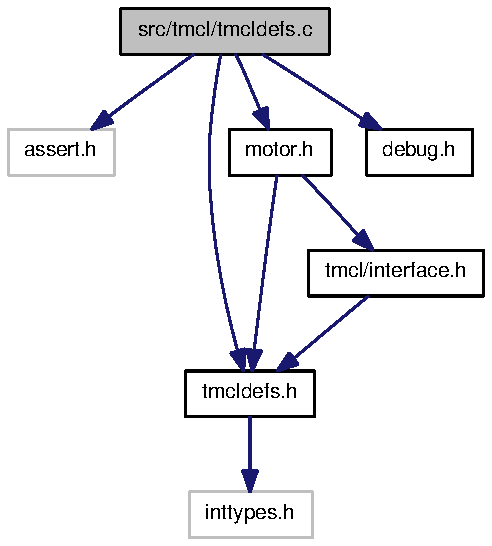
\includegraphics[width=136pt]{tmcldefs_8c__incl}
\end{center}
\end{figure}
\subsection*{Functions}
\begin{DoxyCompactItemize}
\item 
void \hyperlink{tmcldefs_8c_a27ed85719d320cef5cef2b90868bbb9c}{tmcl\_\-init} (\hyperlink{structTMCLDeviceStruct}{TMCLDevice} $\ast$device)
\item 
void \hyperlink{tmcldefs_8c_ad20a3fa13e8e47d01b384ff9658fdf33}{tmcl\_\-deinit} (\hyperlink{structTMCLDeviceStruct}{TMCLDevice} $\ast$device)
\item 
uint8\_\-t \hyperlink{tmcldefs_8c_a5920c3af8a37f1de4af706aeeadff94a}{tmcl\_\-checksum} (uint8\_\-t $\ast$commands, int length)
\item 
int \hyperlink{tmcldefs_8c_a2e979701c691c92a81b197fe775a9294}{tmcl\_\-datagram} (uint8\_\-t $\ast$datagram, \hyperlink{structTMCLDeviceStruct}{TMCLDevice} device, uint8\_\-t command, uint8\_\-t type, uint32\_\-t value)
\item 
int \hyperlink{tmcldefs_8c_a371acd071416d76bde976505cc49ad25}{tmcl\_\-valid\_\-checksum} (\hyperlink{structTMCLReplyStruct}{TMCLReply} reply)
\item 
int \hyperlink{tmcldefs_8c_a5b33e3430cd2cd2c99dbdc71f49737a8}{tmcl\_\-dgram2reply} (\hyperlink{structTMCLReplyStruct}{TMCLReply} $\ast$reply, uint8\_\-t $\ast$datagram, int length)
\end{DoxyCompactItemize}


\subsection{Detailed Description}
Internal functions 

Definition in file \hyperlink{tmcldefs_8c_source}{tmcldefs.c}.

\subsection{Function Documentation}
\hypertarget{tmcldefs_8c_a5920c3af8a37f1de4af706aeeadff94a}{
\index{tmcldefs.c@{tmcldefs.c}!tmcl\_\-checksum@{tmcl\_\-checksum}}
\index{tmcl\_\-checksum@{tmcl\_\-checksum}!tmcldefs.c@{tmcldefs.c}}
\subsubsection[{tmcl\_\-checksum}]{\setlength{\rightskip}{0pt plus 5cm}uint8\_\-t tmcl\_\-checksum (uint8\_\-t $\ast$ {\em commands}, \/  int {\em length})}}
\label{tmcldefs_8c_a5920c3af8a37f1de4af706aeeadff94a}

\begin{DoxyParams}{Parameters}
\item[{\em commands}]Buffer containing the datagram \item[{\em length}]length of datagram \end{DoxyParams}
\begin{DoxyReturn}{Returns}
Checksum 
\end{DoxyReturn}
\begin{DoxySeeAlso}{See also}
\hyperlink{group__TMCLMisc_ga7d2c47709a2fef9913f9c4000d68c814}{TMCL\_\-DGRAM\_\-SIZE\_\-CAN}, \hyperlink{group__TMCLMisc_ga893fbfdcd1c9af739173be6476ad1696}{TMCL\_\-DGRAM\_\-SIZE\_\-RSXXX}, \hyperlink{group__TMCLMisc_gac361bd7186e0b9243b2a8d6dbd465660}{TMCL\_\-DGRAM\_\-SIZE\_\-IIC} 
\end{DoxySeeAlso}


Definition at line 61 of file tmcldefs.c.\hypertarget{tmcldefs_8c_a2e979701c691c92a81b197fe775a9294}{
\index{tmcldefs.c@{tmcldefs.c}!tmcl\_\-datagram@{tmcl\_\-datagram}}
\index{tmcl\_\-datagram@{tmcl\_\-datagram}!tmcldefs.c@{tmcldefs.c}}
\subsubsection[{tmcl\_\-datagram}]{\setlength{\rightskip}{0pt plus 5cm}int tmcl\_\-datagram (uint8\_\-t $\ast$ {\em datagram}, \/  {\bf TMCLDevice} {\em device}, \/  uint8\_\-t {\em command}, \/  uint8\_\-t {\em type}, \/  uint32\_\-t {\em value})}}
\label{tmcldefs_8c_a2e979701c691c92a81b197fe775a9294}

\begin{DoxyParams}{Parameters}
\item[{\em datagram}]Buffer to store the datagram \item[{\em device}]The device for which the datagram is intended \item[{\em command}]The \hyperlink{group__TMCLComm}{command} \item[{\em type}]Type \item[{\em value}]Value \end{DoxyParams}
\begin{DoxyReturn}{Returns}
Length of datagram 
\end{DoxyReturn}
\begin{DoxySeeAlso}{See also}
\hyperlink{group__TMCLComm}{TMCL Commands} 
\end{DoxySeeAlso}


Definition at line 82 of file tmcldefs.c.\hypertarget{tmcldefs_8c_ad20a3fa13e8e47d01b384ff9658fdf33}{
\index{tmcldefs.c@{tmcldefs.c}!tmcl\_\-deinit@{tmcl\_\-deinit}}
\index{tmcl\_\-deinit@{tmcl\_\-deinit}!tmcldefs.c@{tmcldefs.c}}
\subsubsection[{tmcl\_\-deinit}]{\setlength{\rightskip}{0pt plus 5cm}void tmcl\_\-deinit ({\bf TMCLDevice} $\ast$ {\em device})}}
\label{tmcldefs_8c_ad20a3fa13e8e47d01b384ff9658fdf33}
\begin{Desc}
\item[\hyperlink{todo__todo000003}{Todo}]Document this. \end{Desc}


Definition at line 48 of file tmcldefs.c.\hypertarget{tmcldefs_8c_a5b33e3430cd2cd2c99dbdc71f49737a8}{
\index{tmcldefs.c@{tmcldefs.c}!tmcl\_\-dgram2reply@{tmcl\_\-dgram2reply}}
\index{tmcl\_\-dgram2reply@{tmcl\_\-dgram2reply}!tmcldefs.c@{tmcldefs.c}}
\subsubsection[{tmcl\_\-dgram2reply}]{\setlength{\rightskip}{0pt plus 5cm}int tmcl\_\-dgram2reply ({\bf TMCLReply} $\ast$ {\em reply}, \/  uint8\_\-t $\ast$ {\em datagram}, \/  int {\em length})}}
\label{tmcldefs_8c_a5b33e3430cd2cd2c99dbdc71f49737a8}

\begin{DoxyParams}{Parameters}
\item[{\em reply}]tmcl\_\-reply structure to store the data \item[{\em datagram}]The datagram received from the module \item[{\em length}]Lengh of the datagram \end{DoxyParams}
\begin{DoxyReturn}{Returns}

\begin{DoxyItemize}
\item 0 on success
\item -\/1 undefined length 
\end{DoxyItemize}
\end{DoxyReturn}


Definition at line 172 of file tmcldefs.c.\hypertarget{tmcldefs_8c_a27ed85719d320cef5cef2b90868bbb9c}{
\index{tmcldefs.c@{tmcldefs.c}!tmcl\_\-init@{tmcl\_\-init}}
\index{tmcl\_\-init@{tmcl\_\-init}!tmcldefs.c@{tmcldefs.c}}
\subsubsection[{tmcl\_\-init}]{\setlength{\rightskip}{0pt plus 5cm}void tmcl\_\-init ({\bf TMCLDevice} $\ast$ {\em device})}}
\label{tmcldefs_8c_a27ed85719d320cef5cef2b90868bbb9c}
\begin{Desc}
\item[\hyperlink{todo__todo000002}{Todo}]Document this. \end{Desc}


Definition at line 35 of file tmcldefs.c.\hypertarget{tmcldefs_8c_a371acd071416d76bde976505cc49ad25}{
\index{tmcldefs.c@{tmcldefs.c}!tmcl\_\-valid\_\-checksum@{tmcl\_\-valid\_\-checksum}}
\index{tmcl\_\-valid\_\-checksum@{tmcl\_\-valid\_\-checksum}!tmcldefs.c@{tmcldefs.c}}
\subsubsection[{tmcl\_\-valid\_\-checksum}]{\setlength{\rightskip}{0pt plus 5cm}int tmcl\_\-valid\_\-checksum ({\bf TMCLReply} {\em reply})}}
\label{tmcldefs_8c_a371acd071416d76bde976505cc49ad25}

\begin{DoxyParams}{Parameters}
\item[{\em reply}]The reply of the module \end{DoxyParams}
\begin{DoxyReturn}{Returns}

\begin{DoxyItemize}
\item 1 on good checksum
\item 0 on bad checksum 
\end{DoxyItemize}
\end{DoxyReturn}


Definition at line 138 of file tmcldefs.c.
\hypertarget{tmcldefs_8h}{
\section{src/tmcl/tmcldefs.h File Reference}
\label{tmcldefs_8h}\index{src/tmcl/tmcldefs.h@{src/tmcl/tmcldefs.h}}
}
{\ttfamily \#include $<$inttypes.h$>$}\par
Include dependency graph for tmcldefs.h:\nopagebreak
\begin{figure}[H]
\begin{center}
\leavevmode
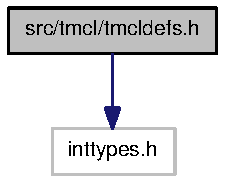
\includegraphics[width=72pt]{tmcldefs_8h__incl}
\end{center}
\end{figure}
This graph shows which files directly or indirectly include this file:\nopagebreak
\begin{figure}[H]
\begin{center}
\leavevmode
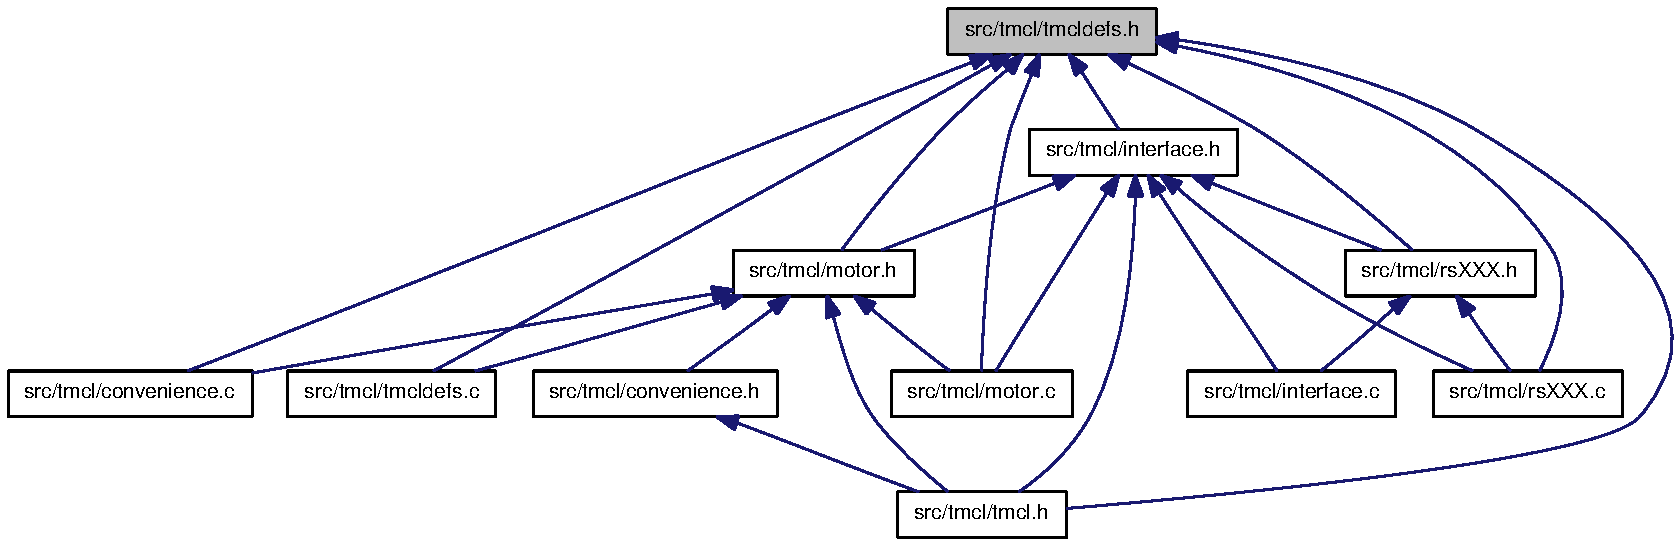
\includegraphics[width=420pt]{tmcldefs_8h__dep__incl}
\end{center}
\end{figure}
\subsection*{Data Structures}
\begin{DoxyCompactItemize}
\item 
struct \hyperlink{structTMCLDeviceStruct}{TMCLDeviceStruct}
\item 
struct \hyperlink{structTMCLReplyStruct}{TMCLReplyStruct}
\item 
struct \hyperlink{structTMCLCommandStruct}{TMCLCommandStruct}
\end{DoxyCompactItemize}
\subsection*{Defines}
\begin{DoxyCompactItemize}
\item 
\hypertarget{tmcldefs_8h_ac5c6df1cce89a8dcd6bd81837eb4934a}{
\#define {\bfseries \_\-\_\-TMCL\_\-TMCLDEFS\_\-H\_\-}~1}
\label{tmcldefs_8h_ac5c6df1cce89a8dcd6bd81837eb4934a}

\item 
\#define \hyperlink{group__TMCLMisc_ga420f7d4b6299372763e4ac6ca6d4919a}{TMCL\_\-VERSION}~3.27
\item 
\#define \hyperlink{group__TMCLMisc_ga7d2c47709a2fef9913f9c4000d68c814}{TMCL\_\-DGRAM\_\-SIZE\_\-CAN}~7
\item 
\#define \hyperlink{group__TMCLMisc_gac361bd7186e0b9243b2a8d6dbd465660}{TMCL\_\-DGRAM\_\-SIZE\_\-IIC}~8
\item 
\#define \hyperlink{group__TMCLMisc_ga893fbfdcd1c9af739173be6476ad1696}{TMCL\_\-DGRAM\_\-SIZE\_\-RSXXX}~9
\item 
\#define \hyperlink{group__TMCLMisc_gad1cf3cae816b86b67bb50098b690a010}{TMCL\_\-MAX\_\-DGRAM\_\-SIZE}~TMCL\_\-DGRAM\_\-SIZE\_\-RSXXX
\item 
\hypertarget{tmcldefs_8h_aae669e3d19a319c69330de57574c24b9}{
\#define {\bfseries TMCL\_\-MAX\_\-PAR\_\-NO}~211}
\label{tmcldefs_8h_aae669e3d19a319c69330de57574c24b9}

\item 
\#define \hyperlink{group__StatusCodes_gae8f0d829c003e2daf2b4d659f10fb365}{TMCL\_\-STATUS\_\-SUCCESS}~100
\item 
\#define \hyperlink{group__StatusCodes_gae781af2133cc40ed37e50627769f75f3}{TMCL\_\-STATUS\_\-LOADED\_\-EEPROM}~101
\item 
\#define \hyperlink{group__StatusCodes_gaf588b372da14d242fc4ecb4e144b5085}{TMCL\_\-STATUS\_\-WRONG\_\-CHECKSUM}~1
\item 
\#define \hyperlink{group__StatusCodes_ga61d064f4c9f910aeb110a92489664d48}{TMCL\_\-STATUS\_\-INVALID\_\-COMMAND}~2
\item 
\#define \hyperlink{group__StatusCodes_ga9fffa59df78430367ff93cabf36f72c6}{TMCL\_\-STATUS\_\-WRONG\_\-TYPE}~3
\item 
\#define \hyperlink{group__StatusCodes_ga0d34bdc73a05adf2c2bc7e6038fb6c64}{TMCL\_\-STATUS\_\-INVALID\_\-VALUE}~4
\item 
\#define \hyperlink{group__StatusCodes_gab3c467b9ae2a256a4d62dd4e7e1922af}{TMCL\_\-STATUS\_\-EEPROM\_\-LOCKED}~5
\item 
\#define \hyperlink{group__StatusCodes_gade3c304cd225d35cad340c7fdff3a801}{TMCL\_\-STATUS\_\-COMMAND\_\-NA}~6
\item 
\#define \hyperlink{group__MotionComm_gae60969d45c586023c9bd2db9498cc508}{TMCL\_\-ROR}~1
\item 
\#define \hyperlink{group__MotionComm_ga90f30df41b6fa29a3e94c909e655af94}{TMCL\_\-ROL}~2
\item 
\#define \hyperlink{group__MotionComm_ga94462741a6a5efcf6b175294cb9b6ecf}{TMCL\_\-MST}~3
\item 
\#define \hyperlink{group__MotionComm_ga109d51fee8df715b9e18b6c49b785757}{TMCL\_\-MVP}~4
\item 
\#define \hyperlink{group__MotionComm_ga316ddf99f164783c8488c48ce9346c21}{TMCL\_\-RFS}~13
\item 
\#define \hyperlink{group__ParComm_ga9d041a48b17f51e16e6219d3cfe5a2ca}{TMCL\_\-SAP}~5
\item 
\#define \hyperlink{group__ParComm_gaeac28ca289b13b735506291521646a4a}{TMCL\_\-GAP}~6
\item 
\#define \hyperlink{group__ParComm_ga22d01b4d2941ab2a2881f17975424f41}{TMCL\_\-STAP}~7
\item 
\#define \hyperlink{group__ParComm_gab338e76ee77e5f122d1694c728beb5e3}{TMCL\_\-RSAP}~8
\item 
\#define \hyperlink{group__ParComm_ga12919729038b159bb1f9b275c9c8f5bc}{TMCL\_\-SGP}~9
\item 
\#define \hyperlink{group__ParComm_ga4bf884d087a29a85073718bbd0d4f928}{TMCL\_\-GGP}~10
\item 
\#define \hyperlink{group__ParComm_ga209b905332339e2b52a7166f46ef2db9}{TMCL\_\-STGP}~11
\item 
\#define \hyperlink{group__ParComm_ga21517120fb13310ef4416fd370fa91b6}{TMCL\_\-RSGP}~12
\item 
\#define \hyperlink{group__TMCLComm_gac92473e5d6624712eb0c6e3b96e72556}{TMCL\_\-SIO}~14
\item 
\#define \hyperlink{group__TMCLComm_gaf8c91f7e3398565e620f87695e2ac8aa}{TMCL\_\-GIO}~15
\item 
\#define \hyperlink{group__TMCLComm_gaaca5ca8ff4397dde2a1d974a08dfc97d}{TMCL\_\-CALC}~19
\item 
\#define \hyperlink{group__TMCLComm_gab3445bd6ed45c31f3ed3f4db49914bbd}{TMCL\_\-COMP}~20
\item 
\#define \hyperlink{group__TMCLComm_gae98b22b798475ff3262efec2168b98a1}{TMCL\_\-JC}~21
\item 
\#define \hyperlink{group__TMCLComm_ga7516bcd7048ea0be08c282cfb65232dc}{TMCL\_\-JA}~22
\item 
\#define \hyperlink{group__TMCLComm_ga42c0ac92b2357e8833d3294b36f3ce03}{TMCL\_\-CSUB}~23
\item 
\#define \hyperlink{group__TMCLComm_gab5dbf5f5909e2c59d70ddf48dd6d68fe}{TMCL\_\-RSUB}~24
\item 
\#define \hyperlink{group__TMCLComm_ga3c134dcd5083b786adf60d3240cdee87}{TMCL\_\-WAIT}~27
\item 
\#define \hyperlink{group__TMCLComm_ga85496061c9785e9cc81068564f72d11a}{TMCL\_\-STOP}~28
\item 
\#define \hyperlink{group__TMCLComm_gaa5bb837c0debc7de9548dcd55f233cda}{TMCL\_\-SAC}~29
\item 
\#define \hyperlink{group__TMCLComm_ga98541d48d1c0ae966624414f02869164}{TMCL\_\-SCO}~30
\item 
\#define \hyperlink{group__TMCLComm_gadfdbd63f01a0e7148e6ad2ac5c7aa3f1}{TMCL\_\-GCO}~31
\item 
\#define \hyperlink{group__TMCLComm_ga55f02944bc20337ded009ae3a22a2e19}{TMCL\_\-CCO}~32
\item 
\#define \hyperlink{group__TMCLComm_gad58eac496f0281febc26c7302e0f7236}{TMCL\_\-CALCX}~33
\item 
\#define \hyperlink{group__TMCLComm_gadda3b3b029a3c196e05bc3fbb6e9f4c0}{TMCL\_\-AAP}~34
\item 
\#define \hyperlink{group__TMCLComm_gae139fce6d594db73457f09527562468c}{TMCL\_\-AGP}~35
\item 
\#define \hyperlink{group__TMCLComm_gadf8bf4f9343f77c0787ab0f131fbc92a}{TMCL\_\-CLE}~36
\item 
\#define \hyperlink{group__TMCLComm_ga452f379acd2362b3694cc2332a2ad4c0}{TMCL\_\-UF0}~64
\item 
\#define \hyperlink{group__TMCLComm_ga04c7b2800e3c01ac91161f7f680ecea0}{TMCL\_\-UF1}~65
\item 
\#define \hyperlink{group__TMCLComm_ga91dd885d4a0e3d69623d4323ca1d64df}{TMCL\_\-UF2}~66
\item 
\#define \hyperlink{group__TMCLComm_gae6e8731e90f75bc9b1218560f3640926}{TMCL\_\-UF3}~67
\item 
\#define \hyperlink{group__TMCLComm_ga24ceb335f6461de5fb3c2bd27cbb7823}{TMCL\_\-UF4}~68
\item 
\#define \hyperlink{group__TMCLComm_ga76c1ecb8e0999fac3d42b5ae4e8cc076}{TMCL\_\-UF5}~69
\item 
\#define \hyperlink{group__TMCLComm_gab5c21ab342d5fd4f5df3f5a0b286ccd1}{TMCL\_\-UF6}~70
\item 
\#define \hyperlink{group__TMCLComm_gaf16a383aac035a9bcf695ecd66ca8df2}{TMCL\_\-UF7}~71
\item 
\#define \hyperlink{group__CTLFuncs_gaa9e1148b7664ea0b5a78f845332b4fd7}{TMCL\_\-CTL\_\-STOP}~128
\item 
\#define \hyperlink{group__CTLFuncs_ga22166cf0f91912ea37048297d8030247}{TMCL\_\-CTL\_\-RUN}~129
\item 
\#define \hyperlink{group__CTLFuncs_ga0ffb8262b5b83a477e839844789fe986}{TMCL\_\-CTL\_\-STEP}~130
\item 
\#define \hyperlink{group__CTLFuncs_ga433f27b92ba499465f7eab488fbd3cea}{TMCL\_\-CTL\_\-RST}~131
\item 
\#define \hyperlink{group__CTLFuncs_gab0ffec97bdd896d0d98eacf2c80ac946}{TMCL\_\-CTL\_\-DLM\_\-START}~132
\item 
\#define \hyperlink{group__CTLFuncs_gaff3c81037366905174f34c8406f058c7}{TMCL\_\-CTL\_\-DLM\_\-QUIT}~133
\item 
\#define \hyperlink{group__CTLFuncs_ga9d883e9bae5236c285877f884bb8a613}{TMCL\_\-CTL\_\-READMEM}~134
\item 
\#define \hyperlink{group__CTLFuncs_gaf8364761b483fed9c95abaedffcf0ec2}{TMCL\_\-CTL\_\-STATUS}~135
\item 
\#define \hyperlink{group__CTLFuncs_gaac0228cc9a707b904b510de74a7fb505}{TMCL\_\-CTL\_\-FW\_\-VER}~136
\item 
\#define \hyperlink{group__CTLFuncs_gab41e9c01de441b30b228801e51243895}{TMCL\_\-CTL\_\-FACTORY}~137
\item 
\#define \hyperlink{group__CTLFuncs_ga36f62eadca8ba64c832ac6120f5a372a}{TMCL\_\-CTL\_\-ASCII}~139
\item 
\#define \hyperlink{group__TMCLComm_gafb1f96d5d46a081eaafdf4d8172e5417}{TMCL\_\-MVP\_\-ABS}~0
\item 
\#define \hyperlink{group__TMCLComm_gabb48ea6fc019299ba3081da7be7a1cdb}{TMCL\_\-MVP\_\-REL}~1
\item 
\#define \hyperlink{group__TMCLComm_gab1bd55bf2087a0fa580a7ed196b731b2}{TMCL\_\-MVP\_\-COORD}~2
\item 
\#define \hyperlink{group__TMCLComm_ga8ecbfcad4ab934cc6b3b4c90f07a5ba6}{TMCL\_\-RFS\_\-START}~0
\item 
\#define \hyperlink{group__TMCLComm_gadad6e89adaf4b2c93c8afd785b3aeb29}{TMCL\_\-RFS\_\-STOP}~1
\item 
\#define \hyperlink{group__TMCLComm_gadc8231e2815a936cb84f36f75da3ca02}{TMCL\_\-RFS\_\-STATUS}~2
\item 
\#define \hyperlink{group__RWParam_ga87dfb3db656c898683ae4a5dd80e789a}{TMCL\_\-AP\_\-TARGET\_\-POS}~0
\item 
\#define \hyperlink{group__RWParam_ga46ffdf772b16b88c99f5b48893b3f710}{TMCL\_\-AP\_\-CURR\_\-POS}~1
\item 
\#define \hyperlink{group__RWParam_ga9f34f155a65163069922f5f20c4c63b5}{TMCL\_\-AP\_\-TARGET\_\-SPEED}~2
\item 
\#define \hyperlink{group__RWParam_gafeecf0d7ec4c89beea4eb6e5dd3d5326}{TMCL\_\-AP\_\-MAX\_\-POS\_\-SPEED}~4
\item 
\#define \hyperlink{group__RWParam_ga5f18e570598b33d3d77b0d0894d81dc7}{TMCL\_\-AP\_\-MAX\_\-ACCEL}~5
\item 
\#define \hyperlink{group__RWParam_gaaf8d5010f2cf9799b5321358b5f5fb35}{TMCL\_\-AP\_\-ABS\_\-CURRENT}~6
\item 
\#define \hyperlink{group__RWParam_ga7e4a74f86decbbced917fb7825aef450}{TMCL\_\-AP\_\-STBY\_\-CURRENT}~7
\item 
\#define \hyperlink{group__RWParam_ga126f3a0bebd82760451aeadab91d6e06}{TMCL\_\-AP\_\-DISABLE\_\-LIMIT\_\-R}~12
\item 
\#define \hyperlink{group__RWParam_ga36067071d35368d2a1b03ddfae1d4eb9}{TMCL\_\-AP\_\-DISABLE\_\-LIMIT\_\-L}~13
\item 
\#define \hyperlink{group__RWParam_gab96353fcd1f433ef38ea445f812d2616}{TMCL\_\-AP\_\-SR\_\-PRESC}~14
\item 
\#define \hyperlink{group__RWParam_gaaf9500c37e13a506bcebb07378bb559c}{TMCL\_\-AP\_\-MICROSTEPS}~140
\item 
\#define \hyperlink{group__RWParam_ga6c4829576ea5ead497c9fd6bc564ecf0}{TMCL\_\-AP\_\-MAX\_\-CURR\_\-REST}~143
\item 
\#define \hyperlink{group__RWParam_gad989938d2101b5e000d5f41ca1d2a522}{TMCL\_\-AP\_\-MAX\_\-CURR\_\-LOW\_\-ACCEL}~144
\item 
\#define \hyperlink{group__RWParam_ga1a3faf0da53cb9d7cc2a84cc326ccc4a}{TMCL\_\-AP\_\-MAX\_\-CURR\_\-HIGH\_\-ACCEL}~145
\item 
\#define \hyperlink{group__RWParam_gaf504e536f23e990387a1b4421fcc49e4}{TMCL\_\-AP\_\-RFS\_\-MODE}~193
\item 
\#define \hyperlink{group__RWParam_ga4c6ebda674b3ce393db587761c169515}{TMCL\_\-AP\_\-RFS\_\-SPEED}~194
\item 
\#define \hyperlink{group__RWParam_ga31404aaf7195272cd4a6ef150d6ea421}{TMCL\_\-AP\_\-RFS\_\-SW\_\-SPEED}~195
\item 
\#define \hyperlink{group__ROParam_ga3473b35e8f38849da91e101a751b474d}{TMCL\_\-AP\_\-CURR\_\-SPEED}~3
\item 
\#define \hyperlink{group__ROParam_ga8340c6753a1858eae01d9a7a0f1ea221}{TMCL\_\-AP\_\-POS\_\-REACHED}~8
\item 
\#define \hyperlink{group__ROParam_ga389a6e3b6ba6e1bc1ad719f055bf139f}{TMCL\_\-AP\_\-LIMIT\_\-R}~9
\item 
\#define \hyperlink{group__ROParam_ga4751b3398d03d02e756d6b564a735b51}{TMCL\_\-AP\_\-LIMIT\_\-L}~10
\end{DoxyCompactItemize}
\subsection*{Typedefs}
\begin{DoxyCompactItemize}
\item 
typedef int32\_\-t \hyperlink{tmcldefs_8h_a1c27da9ad00f668a659641ec0b94b9ce}{TMCLParameter}
\item 
\hypertarget{tmcldefs_8h_af6bebda82514db085eba2fb6711976cc}{
typedef \hyperlink{tmcldefs_8h_a1c27da9ad00f668a659641ec0b94b9ce}{TMCLParameter} {\bfseries TMCLParameters} \mbox{[}TMCL\_\-MAX\_\-PAR\_\-NO+1\mbox{]}}
\label{tmcldefs_8h_af6bebda82514db085eba2fb6711976cc}

\item 
typedef enum \hyperlink{tmcldefs_8h_a3c0af0cc3f62b9e4a1daea7839da918e}{tmcl\_\-busses} \hyperlink{tmcldefs_8h_ad26e4e286a55d7c739fd473d8cdd882e}{TMCLBusType}
\item 
typedef enum \hyperlink{tmcldefs_8h_a5b6ac18c2401b554e24fe3313eda6e9a}{TMCLModelEnum} \hyperlink{tmcldefs_8h_a35c090090de43d9850d0f573f7d29e45}{TMCLModel}
\item 
typedef struct \hyperlink{structTMCLDeviceStruct}{TMCLDeviceStruct} \hyperlink{tmcldefs_8h_adf97b172ea75c2fd91bf4ab98f65ffea}{TMCLDevice}
\item 
typedef struct \hyperlink{structTMCLReplyStruct}{TMCLReplyStruct} \hyperlink{tmcldefs_8h_ac5261105efa5a31da90627f0cb2153d2}{TMCLReply}
\item 
typedef struct \hyperlink{structTMCLCommandStruct}{TMCLCommandStruct} \hyperlink{tmcldefs_8h_a61ff3e5938eeb8d7a5b41fcba8f7c914}{TMCLCommand}
\end{DoxyCompactItemize}
\subsection*{Enumerations}
\begin{DoxyCompactItemize}
\item 
enum \hyperlink{tmcldefs_8h_a3c0af0cc3f62b9e4a1daea7839da918e}{tmcl\_\-busses} \{ \hyperlink{tmcldefs_8h_a3c0af0cc3f62b9e4a1daea7839da918eaf9dbccd234fb0d6fa5cc9e228e3219fd}{TMCL\_\-CAN}, 
\hyperlink{tmcldefs_8h_a3c0af0cc3f62b9e4a1daea7839da918eaeebe71669361b77c7409940d04d22cc5}{TMCL\_\-RSXXX}, 
\hyperlink{tmcldefs_8h_a3c0af0cc3f62b9e4a1daea7839da918ea27b661ff5f5dd238584fb2765764c314}{TMCL\_\-IIC}, 
\hyperlink{tmcldefs_8h_a3c0af0cc3f62b9e4a1daea7839da918eae1c14eefd4ba053ee83ed080d85c8971}{TMCL\_\-NONE}
 \}
\item 
enum \hyperlink{tmcldefs_8h_a5b6ac18c2401b554e24fe3313eda6e9a}{TMCLModelEnum} \{ \par
\hyperlink{tmcldefs_8h_a5b6ac18c2401b554e24fe3313eda6e9aacf81076a68a2e93d0d78e11c3c241a65}{TMCM300}, 
\hyperlink{tmcldefs_8h_a5b6ac18c2401b554e24fe3313eda6e9aa8e6b450903c9e2cae2e5eb99e3e74467}{TMCM301}, 
\hyperlink{tmcldefs_8h_a5b6ac18c2401b554e24fe3313eda6e9aa8bdcff6dcfcf488fc958ca47ecfd19cb}{TMCM302}, 
\hyperlink{tmcldefs_8h_a5b6ac18c2401b554e24fe3313eda6e9aa31f54f81317e016a8f3596d0e81b0396}{TMCM303}, 
\par
\hyperlink{tmcldefs_8h_a5b6ac18c2401b554e24fe3313eda6e9aace134b21b8249de1085743749015c3d3}{TMCM310}, 
\hyperlink{tmcldefs_8h_a5b6ac18c2401b554e24fe3313eda6e9aa387914281e7a40ff81cf1906ae4b938b}{TMCM11x}, 
\hyperlink{tmcldefs_8h_a5b6ac18c2401b554e24fe3313eda6e9aaba0fcc6b784d4e85e25095b304373869}{TMCM109}, 
\hyperlink{tmcldefs_8h_a5b6ac18c2401b554e24fe3313eda6e9aafdf19449aaf1bf2abcac9ee1e58a3207}{TMCM110}, 
\par
\hyperlink{tmcldefs_8h_a5b6ac18c2401b554e24fe3313eda6e9aa9a54f297ca02c20ceabebc926a90d5ae}{TMCM100}, 
\hyperlink{tmcldefs_8h_a5b6ac18c2401b554e24fe3313eda6e9aa4d0773732a828d83cc129067791f65a4}{TMCM610}, 
\hyperlink{tmcldefs_8h_a5b6ac18c2401b554e24fe3313eda6e9aa04fd42d7ff7fcaea62ef4ce5b068f490}{TMCM611}, 
\hyperlink{tmcldefs_8h_a5b6ac18c2401b554e24fe3313eda6e9aa7cfc6fad718d6e52e83c608c794953cb}{TMCM612}
 \}
\end{DoxyCompactItemize}
\subsection*{Functions}
\begin{DoxyCompactItemize}
\item 
void \hyperlink{tmcldefs_8h_a4843aec6363ff7b374b5fe190e17fe6e}{tmcl\_\-init} (\hyperlink{structTMCLDeviceStruct}{TMCLDevice} $\ast$)
\item 
void \hyperlink{tmcldefs_8h_a59f577127efc6cc200f6212a19b75f62}{tmcl\_\-deinit} (\hyperlink{structTMCLDeviceStruct}{TMCLDevice} $\ast$)
\item 
uint8\_\-t \hyperlink{tmcldefs_8h_aa22a7985c0afc7af2f169f47be7aa3d1}{tmcl\_\-checksum} (uint8\_\-t $\ast$, int)
\item 
int \hyperlink{tmcldefs_8h_a8ae83ae40ca930afde6db90ea0b9cb5c}{tmcl\_\-datagram} (uint8\_\-t $\ast$, \hyperlink{structTMCLDeviceStruct}{TMCLDevice}, uint8\_\-t, uint8\_\-t, uint32\_\-t)
\item 
int \hyperlink{tmcldefs_8h_a36bab56c5448f75e81543f5e1d5855dc}{tmcl\_\-valid\_\-checksum} (\hyperlink{structTMCLReplyStruct}{TMCLReply})
\item 
int \hyperlink{tmcldefs_8h_a946609ef74e832b772d1047f5cd809d0}{tmcl\_\-dgram2reply} (\hyperlink{structTMCLReplyStruct}{TMCLReply} $\ast$, uint8\_\-t $\ast$, int)
\end{DoxyCompactItemize}


\subsection{Detailed Description}
Definitions for TMCLlib 

Definition in file \hyperlink{tmcldefs_8h_source}{tmcldefs.h}.

\subsection{Typedef Documentation}
\hypertarget{tmcldefs_8h_ad26e4e286a55d7c739fd473d8cdd882e}{
\index{tmcldefs.h@{tmcldefs.h}!TMCLBusType@{TMCLBusType}}
\index{TMCLBusType@{TMCLBusType}!tmcldefs.h@{tmcldefs.h}}
\subsubsection[{TMCLBusType}]{\setlength{\rightskip}{0pt plus 5cm}typedef enum {\bf tmcl\_\-busses}  {\bf TMCLBusType}}}
\label{tmcldefs_8h_ad26e4e286a55d7c739fd473d8cdd882e}
Supported busses and interfaces. \hypertarget{tmcldefs_8h_a61ff3e5938eeb8d7a5b41fcba8f7c914}{
\index{tmcldefs.h@{tmcldefs.h}!TMCLCommand@{TMCLCommand}}
\index{TMCLCommand@{TMCLCommand}!tmcldefs.h@{tmcldefs.h}}
\subsubsection[{TMCLCommand}]{\setlength{\rightskip}{0pt plus 5cm}typedef struct {\bf TMCLCommandStruct}  {\bf TMCLCommand}}}
\label{tmcldefs_8h_a61ff3e5938eeb8d7a5b41fcba8f7c914}
Structure containing a TMCL command and related data.

\begin{DoxySeeAlso}{See also}
\hyperlink{group__TMCLComm}{TMCL commands.} 
\end{DoxySeeAlso}
\hypertarget{tmcldefs_8h_adf97b172ea75c2fd91bf4ab98f65ffea}{
\index{tmcldefs.h@{tmcldefs.h}!TMCLDevice@{TMCLDevice}}
\index{TMCLDevice@{TMCLDevice}!tmcldefs.h@{tmcldefs.h}}
\subsubsection[{TMCLDevice}]{\setlength{\rightskip}{0pt plus 5cm}typedef struct {\bf TMCLDeviceStruct}  {\bf TMCLDevice}}}
\label{tmcldefs_8h_adf97b172ea75c2fd91bf4ab98f65ffea}
Information of the TMCL module.

\begin{DoxySeeAlso}{See also}
\hyperlink{tmcldefs_8h_ad26e4e286a55d7c739fd473d8cdd882e}{TMCLBusType} 
\end{DoxySeeAlso}
\hypertarget{tmcldefs_8h_a35c090090de43d9850d0f573f7d29e45}{
\index{tmcldefs.h@{tmcldefs.h}!TMCLModel@{TMCLModel}}
\index{TMCLModel@{TMCLModel}!tmcldefs.h@{tmcldefs.h}}
\subsubsection[{TMCLModel}]{\setlength{\rightskip}{0pt plus 5cm}typedef enum {\bf TMCLModelEnum}  {\bf TMCLModel}}}
\label{tmcldefs_8h_a35c090090de43d9850d0f573f7d29e45}
Supported TMCL Device Models \hypertarget{tmcldefs_8h_a1c27da9ad00f668a659641ec0b94b9ce}{
\index{tmcldefs.h@{tmcldefs.h}!TMCLParameter@{TMCLParameter}}
\index{TMCLParameter@{TMCLParameter}!tmcldefs.h@{tmcldefs.h}}
\subsubsection[{TMCLParameter}]{\setlength{\rightskip}{0pt plus 5cm}typedef int32\_\-t {\bf TMCLParameter}}}
\label{tmcldefs_8h_a1c27da9ad00f668a659641ec0b94b9ce}
Extended Parameters Storage space for parameter of a device 

Definition at line 225 of file tmcldefs.h.\hypertarget{tmcldefs_8h_ac5261105efa5a31da90627f0cb2153d2}{
\index{tmcldefs.h@{tmcldefs.h}!TMCLReply@{TMCLReply}}
\index{TMCLReply@{TMCLReply}!tmcldefs.h@{tmcldefs.h}}
\subsubsection[{TMCLReply}]{\setlength{\rightskip}{0pt plus 5cm}typedef struct {\bf TMCLReplyStruct}  {\bf TMCLReply}}}
\label{tmcldefs_8h_ac5261105efa5a31da90627f0cb2153d2}
Structure for holding the reply of a module.

\begin{DoxySeeAlso}{See also}
\hyperlink{group__StatusCodes}{Status Codes.}, \hyperlink{group__TMCLComm}{TMCL commands.} 
\end{DoxySeeAlso}


\subsection{Enumeration Type Documentation}
\hypertarget{tmcldefs_8h_a3c0af0cc3f62b9e4a1daea7839da918e}{
\index{tmcldefs.h@{tmcldefs.h}!tmcl\_\-busses@{tmcl\_\-busses}}
\index{tmcl\_\-busses@{tmcl\_\-busses}!tmcldefs.h@{tmcldefs.h}}
\subsubsection[{tmcl\_\-busses}]{\setlength{\rightskip}{0pt plus 5cm}enum {\bf tmcl\_\-busses}}}
\label{tmcldefs_8h_a3c0af0cc3f62b9e4a1daea7839da918e}
Supported busses and interfaces. \begin{Desc}
\item[Enumerator: ]\par
\begin{description}
\index{TMCL\_\-CAN@{TMCL\_\-CAN}!tmcldefs.h@{tmcldefs.h}}\index{tmcldefs.h@{tmcldefs.h}!TMCL\_\-CAN@{TMCL\_\-CAN}}\item[{\em 
\hypertarget{tmcldefs_8h_a3c0af0cc3f62b9e4a1daea7839da918eaf9dbccd234fb0d6fa5cc9e228e3219fd}{
TMCL\_\-CAN}
\label{tmcldefs_8h_a3c0af0cc3f62b9e4a1daea7839da918eaf9dbccd234fb0d6fa5cc9e228e3219fd}
}]CAN bus (currently unsupported) \index{TMCL\_\-RSXXX@{TMCL\_\-RSXXX}!tmcldefs.h@{tmcldefs.h}}\index{tmcldefs.h@{tmcldefs.h}!TMCL\_\-RSXXX@{TMCL\_\-RSXXX}}\item[{\em 
\hypertarget{tmcldefs_8h_a3c0af0cc3f62b9e4a1daea7839da918eaeebe71669361b77c7409940d04d22cc5}{
TMCL\_\-RSXXX}
\label{tmcldefs_8h_a3c0af0cc3f62b9e4a1daea7839da918eaeebe71669361b77c7409940d04d22cc5}
}]RS232/RS485 interface \index{TMCL\_\-IIC@{TMCL\_\-IIC}!tmcldefs.h@{tmcldefs.h}}\index{tmcldefs.h@{tmcldefs.h}!TMCL\_\-IIC@{TMCL\_\-IIC}}\item[{\em 
\hypertarget{tmcldefs_8h_a3c0af0cc3f62b9e4a1daea7839da918ea27b661ff5f5dd238584fb2765764c314}{
TMCL\_\-IIC}
\label{tmcldefs_8h_a3c0af0cc3f62b9e4a1daea7839da918ea27b661ff5f5dd238584fb2765764c314}
}]IIC interface (currently unsupported) \index{TMCL\_\-NONE@{TMCL\_\-NONE}!tmcldefs.h@{tmcldefs.h}}\index{tmcldefs.h@{tmcldefs.h}!TMCL\_\-NONE@{TMCL\_\-NONE}}\item[{\em 
\hypertarget{tmcldefs_8h_a3c0af0cc3f62b9e4a1daea7839da918eae1c14eefd4ba053ee83ed080d85c8971}{
TMCL\_\-NONE}
\label{tmcldefs_8h_a3c0af0cc3f62b9e4a1daea7839da918eae1c14eefd4ba053ee83ed080d85c8971}
}]Marker for uninitialized interface \end{description}
\end{Desc}



Definition at line 237 of file tmcldefs.h.\hypertarget{tmcldefs_8h_a5b6ac18c2401b554e24fe3313eda6e9a}{
\index{tmcldefs.h@{tmcldefs.h}!TMCLModelEnum@{TMCLModelEnum}}
\index{TMCLModelEnum@{TMCLModelEnum}!tmcldefs.h@{tmcldefs.h}}
\subsubsection[{TMCLModelEnum}]{\setlength{\rightskip}{0pt plus 5cm}enum {\bf TMCLModelEnum}}}
\label{tmcldefs_8h_a5b6ac18c2401b554e24fe3313eda6e9a}
Supported TMCL Device Models \begin{Desc}
\item[Enumerator: ]\par
\begin{description}
\index{TMCM300@{TMCM300}!tmcldefs.h@{tmcldefs.h}}\index{tmcldefs.h@{tmcldefs.h}!TMCM300@{TMCM300}}\item[{\em 
\hypertarget{tmcldefs_8h_a5b6ac18c2401b554e24fe3313eda6e9aacf81076a68a2e93d0d78e11c3c241a65}{
TMCM300}
\label{tmcldefs_8h_a5b6ac18c2401b554e24fe3313eda6e9aacf81076a68a2e93d0d78e11c3c241a65}
}]TMCM-\/300 \index{TMCM301@{TMCM301}!tmcldefs.h@{tmcldefs.h}}\index{tmcldefs.h@{tmcldefs.h}!TMCM301@{TMCM301}}\item[{\em 
\hypertarget{tmcldefs_8h_a5b6ac18c2401b554e24fe3313eda6e9aa8e6b450903c9e2cae2e5eb99e3e74467}{
TMCM301}
\label{tmcldefs_8h_a5b6ac18c2401b554e24fe3313eda6e9aa8e6b450903c9e2cae2e5eb99e3e74467}
}]TMCM-\/301 \index{TMCM302@{TMCM302}!tmcldefs.h@{tmcldefs.h}}\index{tmcldefs.h@{tmcldefs.h}!TMCM302@{TMCM302}}\item[{\em 
\hypertarget{tmcldefs_8h_a5b6ac18c2401b554e24fe3313eda6e9aa8bdcff6dcfcf488fc958ca47ecfd19cb}{
TMCM302}
\label{tmcldefs_8h_a5b6ac18c2401b554e24fe3313eda6e9aa8bdcff6dcfcf488fc958ca47ecfd19cb}
}]TMCM-\/302 \index{TMCM303@{TMCM303}!tmcldefs.h@{tmcldefs.h}}\index{tmcldefs.h@{tmcldefs.h}!TMCM303@{TMCM303}}\item[{\em 
\hypertarget{tmcldefs_8h_a5b6ac18c2401b554e24fe3313eda6e9aa31f54f81317e016a8f3596d0e81b0396}{
TMCM303}
\label{tmcldefs_8h_a5b6ac18c2401b554e24fe3313eda6e9aa31f54f81317e016a8f3596d0e81b0396}
}]TMCM-\/303 \index{TMCM310@{TMCM310}!tmcldefs.h@{tmcldefs.h}}\index{tmcldefs.h@{tmcldefs.h}!TMCM310@{TMCM310}}\item[{\em 
\hypertarget{tmcldefs_8h_a5b6ac18c2401b554e24fe3313eda6e9aace134b21b8249de1085743749015c3d3}{
TMCM310}
\label{tmcldefs_8h_a5b6ac18c2401b554e24fe3313eda6e9aace134b21b8249de1085743749015c3d3}
}]TMCM-\/310 \index{TMCM11x@{TMCM11x}!tmcldefs.h@{tmcldefs.h}}\index{tmcldefs.h@{tmcldefs.h}!TMCM11x@{TMCM11x}}\item[{\em 
\hypertarget{tmcldefs_8h_a5b6ac18c2401b554e24fe3313eda6e9aa387914281e7a40ff81cf1906ae4b938b}{
TMCM11x}
\label{tmcldefs_8h_a5b6ac18c2401b554e24fe3313eda6e9aa387914281e7a40ff81cf1906ae4b938b}
}]TMCM-\/11x, except TMCL-\/110 \index{TMCM109@{TMCM109}!tmcldefs.h@{tmcldefs.h}}\index{tmcldefs.h@{tmcldefs.h}!TMCM109@{TMCM109}}\item[{\em 
\hypertarget{tmcldefs_8h_a5b6ac18c2401b554e24fe3313eda6e9aaba0fcc6b784d4e85e25095b304373869}{
TMCM109}
\label{tmcldefs_8h_a5b6ac18c2401b554e24fe3313eda6e9aaba0fcc6b784d4e85e25095b304373869}
}]TMCM-\/109 \index{TMCM110@{TMCM110}!tmcldefs.h@{tmcldefs.h}}\index{tmcldefs.h@{tmcldefs.h}!TMCM110@{TMCM110}}\item[{\em 
\hypertarget{tmcldefs_8h_a5b6ac18c2401b554e24fe3313eda6e9aafdf19449aaf1bf2abcac9ee1e58a3207}{
TMCM110}
\label{tmcldefs_8h_a5b6ac18c2401b554e24fe3313eda6e9aafdf19449aaf1bf2abcac9ee1e58a3207}
}]TMCM-\/110 \index{TMCM100@{TMCM100}!tmcldefs.h@{tmcldefs.h}}\index{tmcldefs.h@{tmcldefs.h}!TMCM100@{TMCM100}}\item[{\em 
\hypertarget{tmcldefs_8h_a5b6ac18c2401b554e24fe3313eda6e9aa9a54f297ca02c20ceabebc926a90d5ae}{
TMCM100}
\label{tmcldefs_8h_a5b6ac18c2401b554e24fe3313eda6e9aa9a54f297ca02c20ceabebc926a90d5ae}
}]TMCM-\/100 \index{TMCM610@{TMCM610}!tmcldefs.h@{tmcldefs.h}}\index{tmcldefs.h@{tmcldefs.h}!TMCM610@{TMCM610}}\item[{\em 
\hypertarget{tmcldefs_8h_a5b6ac18c2401b554e24fe3313eda6e9aa4d0773732a828d83cc129067791f65a4}{
TMCM610}
\label{tmcldefs_8h_a5b6ac18c2401b554e24fe3313eda6e9aa4d0773732a828d83cc129067791f65a4}
}]TMCM-\/610 \index{TMCM611@{TMCM611}!tmcldefs.h@{tmcldefs.h}}\index{tmcldefs.h@{tmcldefs.h}!TMCM611@{TMCM611}}\item[{\em 
\hypertarget{tmcldefs_8h_a5b6ac18c2401b554e24fe3313eda6e9aa04fd42d7ff7fcaea62ef4ce5b068f490}{
TMCM611}
\label{tmcldefs_8h_a5b6ac18c2401b554e24fe3313eda6e9aa04fd42d7ff7fcaea62ef4ce5b068f490}
}]TMCM-\/611 \index{TMCM612@{TMCM612}!tmcldefs.h@{tmcldefs.h}}\index{tmcldefs.h@{tmcldefs.h}!TMCM612@{TMCM612}}\item[{\em 
\hypertarget{tmcldefs_8h_a5b6ac18c2401b554e24fe3313eda6e9aa7cfc6fad718d6e52e83c608c794953cb}{
TMCM612}
\label{tmcldefs_8h_a5b6ac18c2401b554e24fe3313eda6e9aa7cfc6fad718d6e52e83c608c794953cb}
}]TMCM-\/612 \end{description}
\end{Desc}



Definition at line 248 of file tmcldefs.h.

\subsection{Function Documentation}
\hypertarget{tmcldefs_8h_aa22a7985c0afc7af2f169f47be7aa3d1}{
\index{tmcldefs.h@{tmcldefs.h}!tmcl\_\-checksum@{tmcl\_\-checksum}}
\index{tmcl\_\-checksum@{tmcl\_\-checksum}!tmcldefs.h@{tmcldefs.h}}
\subsubsection[{tmcl\_\-checksum}]{\setlength{\rightskip}{0pt plus 5cm}uint8\_\-t tmcl\_\-checksum (uint8\_\-t $\ast$ {\em commands}, \/  int {\em length})}}
\label{tmcldefs_8h_aa22a7985c0afc7af2f169f47be7aa3d1}
Calculate the checksum for a datagram


\begin{DoxyParams}{Parameters}
\item[{\em commands}]Buffer containing the datagram \item[{\em length}]length of datagram \end{DoxyParams}
\begin{DoxyReturn}{Returns}
Checksum 
\end{DoxyReturn}
\begin{DoxySeeAlso}{See also}
\hyperlink{group__TMCLMisc_ga7d2c47709a2fef9913f9c4000d68c814}{TMCL\_\-DGRAM\_\-SIZE\_\-CAN}, \hyperlink{group__TMCLMisc_ga893fbfdcd1c9af739173be6476ad1696}{TMCL\_\-DGRAM\_\-SIZE\_\-RSXXX}, \hyperlink{group__TMCLMisc_gac361bd7186e0b9243b2a8d6dbd465660}{TMCL\_\-DGRAM\_\-SIZE\_\-IIC} 
\end{DoxySeeAlso}


Definition at line 61 of file tmcldefs.c.\hypertarget{tmcldefs_8h_a8ae83ae40ca930afde6db90ea0b9cb5c}{
\index{tmcldefs.h@{tmcldefs.h}!tmcl\_\-datagram@{tmcl\_\-datagram}}
\index{tmcl\_\-datagram@{tmcl\_\-datagram}!tmcldefs.h@{tmcldefs.h}}
\subsubsection[{tmcl\_\-datagram}]{\setlength{\rightskip}{0pt plus 5cm}int tmcl\_\-datagram (uint8\_\-t $\ast$ {\em datagram}, \/  {\bf TMCLDevice} {\em device}, \/  uint8\_\-t {\em command}, \/  uint8\_\-t {\em type}, \/  uint32\_\-t {\em value})}}
\label{tmcldefs_8h_a8ae83ae40ca930afde6db90ea0b9cb5c}
Build a datagram for sending to the device.


\begin{DoxyParams}{Parameters}
\item[{\em datagram}]Buffer to store the datagram \item[{\em device}]The device for which the datagram is intended \item[{\em command}]The \hyperlink{group__TMCLComm}{command} \item[{\em type}]Type \item[{\em value}]Value \end{DoxyParams}
\begin{DoxyReturn}{Returns}
Length of datagram 
\end{DoxyReturn}
\begin{DoxySeeAlso}{See also}
\hyperlink{group__TMCLComm}{TMCL Commands} 
\end{DoxySeeAlso}


Definition at line 82 of file tmcldefs.c.\hypertarget{tmcldefs_8h_a59f577127efc6cc200f6212a19b75f62}{
\index{tmcldefs.h@{tmcldefs.h}!tmcl\_\-deinit@{tmcl\_\-deinit}}
\index{tmcl\_\-deinit@{tmcl\_\-deinit}!tmcldefs.h@{tmcldefs.h}}
\subsubsection[{tmcl\_\-deinit}]{\setlength{\rightskip}{0pt plus 5cm}void tmcl\_\-deinit ({\bf TMCLDevice} $\ast$ {\em device})}}
\label{tmcldefs_8h_a59f577127efc6cc200f6212a19b75f62}
Deinitialize TMCLDevice data structure

\begin{Desc}
\item[\hyperlink{todo__todo000003}{Todo}]Document this. \end{Desc}


Definition at line 48 of file tmcldefs.c.\hypertarget{tmcldefs_8h_a946609ef74e832b772d1047f5cd809d0}{
\index{tmcldefs.h@{tmcldefs.h}!tmcl\_\-dgram2reply@{tmcl\_\-dgram2reply}}
\index{tmcl\_\-dgram2reply@{tmcl\_\-dgram2reply}!tmcldefs.h@{tmcldefs.h}}
\subsubsection[{tmcl\_\-dgram2reply}]{\setlength{\rightskip}{0pt plus 5cm}int tmcl\_\-dgram2reply ({\bf TMCLReply} $\ast$ {\em reply}, \/  uint8\_\-t $\ast$ {\em datagram}, \/  int {\em length})}}
\label{tmcldefs_8h_a946609ef74e832b772d1047f5cd809d0}
Convert a datagram received from a module to a tmcl\_\-reply struct.


\begin{DoxyParams}{Parameters}
\item[{\em reply}]tmcl\_\-reply structure to store the data \item[{\em datagram}]The datagram received from the module \item[{\em length}]Lengh of the datagram \end{DoxyParams}
\begin{DoxyReturn}{Returns}

\begin{DoxyItemize}
\item 0 on success
\item -\/1 undefined length 
\end{DoxyItemize}
\end{DoxyReturn}


Definition at line 172 of file tmcldefs.c.\hypertarget{tmcldefs_8h_a4843aec6363ff7b374b5fe190e17fe6e}{
\index{tmcldefs.h@{tmcldefs.h}!tmcl\_\-init@{tmcl\_\-init}}
\index{tmcl\_\-init@{tmcl\_\-init}!tmcldefs.h@{tmcldefs.h}}
\subsubsection[{tmcl\_\-init}]{\setlength{\rightskip}{0pt plus 5cm}void tmcl\_\-init ({\bf TMCLDevice} $\ast$ {\em device})}}
\label{tmcldefs_8h_a4843aec6363ff7b374b5fe190e17fe6e}
Initialize TMCLDevice data structure

\begin{Desc}
\item[\hyperlink{todo__todo000002}{Todo}]Document this. \end{Desc}


Definition at line 35 of file tmcldefs.c.\hypertarget{tmcldefs_8h_a36bab56c5448f75e81543f5e1d5855dc}{
\index{tmcldefs.h@{tmcldefs.h}!tmcl\_\-valid\_\-checksum@{tmcl\_\-valid\_\-checksum}}
\index{tmcl\_\-valid\_\-checksum@{tmcl\_\-valid\_\-checksum}!tmcldefs.h@{tmcldefs.h}}
\subsubsection[{tmcl\_\-valid\_\-checksum}]{\setlength{\rightskip}{0pt plus 5cm}int tmcl\_\-valid\_\-checksum ({\bf TMCLReply} {\em reply})}}
\label{tmcldefs_8h_a36bab56c5448f75e81543f5e1d5855dc}
Check the checksum of a \hyperlink{tmcldefs_8h_ac5261105efa5a31da90627f0cb2153d2}{TMCL reply}


\begin{DoxyParams}{Parameters}
\item[{\em reply}]The reply of the module \end{DoxyParams}
\begin{DoxyReturn}{Returns}

\begin{DoxyItemize}
\item 1 on good checksum
\item 0 on bad checksum 
\end{DoxyItemize}
\end{DoxyReturn}


Definition at line 138 of file tmcldefs.c.
\printindex
\end{document}
